\documentclass[10pt,a4paper]{article}
\usepackage{ngerman}
\usepackage{sectsty, xcolor}
\usepackage{lastpage}
\usepackage{amssymb, enumitem, fancyhdr, graphicx, float, makeidx, textcomp, multicol}
\usepackage[hidelinks]{hyperref}
\usepackage[hang,flushmargin]{footmisc}
\usepackage{authblk} %\author[1]{blub}, \affil[1]{HSLU}
\usepackage{listings}
\lstloadlanguages{SQL}
%%%
%\lstset{language=SQL}
%\begin{lstlisting}
%SELECT * FROM table WHERE id = 1;
%\end{lstlisting}
%%%
\usepackage[backend=biber,style=numeric,sorting=none]{biblatex}
\addbibresource{bibliography.bib}
\makeindex

\definecolor{dunkelblau}{rgb}{0,0.4,0.6}
\subsectionfont{\color{dunkelblau}}

\title{ISF HS 2019}
\author[1]{Victor Fernández}
\author[2]{Hillary Funke}
\author[3]{Pavaskar Parameswaran}
\author[3]{\\Kevin Soares Correia}
\author[2]{Johannen Yilmaz}
\affil[1]{HSLU Informatik}
\affil[2]{HSLU Information and Cybersecurity}
\affil[3]{HSLU Wirtschaftsinformatik}
\date{Dezember 2019}


\addtolength{\oddsidemargin}{-.875in}
\addtolength{\evensidemargin}{-.875in}
\addtolength{\textwidth}{1.75in}
\addtolength{\topmargin}{-.875in}
\addtolength{\textheight}{1.75in}

% muss nach Änderung der margin kommen!
\pagestyle{fancy}
\fancyhf{} %reset
\fancyhead[L]{HSLU}
\fancyhead[C]{ISF}
\fancyhead[R]{\thepage/\pageref{LastPage}}
\fancyfoot[L]{}
\fancyfoot[C]{}
\fancyfoot[R]{}
\renewcommand{\headrulewidth}{0.2pt} % Strich in Kopfzeile

%******
\begin{document}
\maketitle
\thispagestyle{empty}
\section*{Vorwort}Diese Zusammenfassung entstand in einer Gruppe während der Lernphase des HS 2019. Alle Fragen aus der Stoffabgrenzung tragen eine {\color{dunkelblau}blaue Farbe} und stehen als Unterkapitel. Das Dokument ist Open Source und jeder der möchte und signifikant beiträgt, darf sich als Autor anhängen. Die Source ist \underline{\href{https://github.com/vigi86/HSLU_Zusammenfassungen/tree/master/ISF_HS19}{dieses GitHub-Repo}}\footnote{https://github.com/vigi86/HSLU\_Zusammenfassungen/tree/master/ISF\_HS19}. Dies ist mein erstes \LaTeX{}-Dokument überhaupt. Nichts desto trotz wurde auf eine klare Strukturierung und Lesbarkeit des Dokumentes Wert gelegt.
\tableofcontents
\thispagestyle{empty}
\pagebreak


%%%%%%%%%%
\part{Einführung (SW~01)}
\section{Einführung}
\subsection*{Einführung in das Thema "`Management von Informationssicherheit"'}
\paragraph*{Daten, Information und Wissen}
Information ist die Verknüpfung von Daten in Form von Zahlen, Worten und Fakten zu interpretierbaren Zusammenhängen.
Durch die Vernetzung von Informationen entsteht Wissen, das zunächst personenbezogen ist.

\paragraph*{Missbrauch}Informationen müssen vor Missbrauch geschützt werden
\begin{figure}[H]
    \begin{center}
    \includegraphics[width=8cm]{images/Wissenspyramide.png}
    \caption{Wissenspyramide\cite{wiki}}
    \label{Wissenspyramide}
    \end{center}
\end{figure}

\subsection*{Motivation / Bedrohungen}
\paragraph*{Was gefährdet die Informationen?} Welche Gefährdungen/Bedrohungen gibt es?\index{Gefährdungen}\index{Bedrohungen}\index{Informationssicherheit}
\begin{itemize}[noitemsep,topsep=0pt,leftmargin=*]
    \item Nicht vorsätzliche (zufällige) Gefährdungen/Bedrohungen
    \begin{itemize}[noitemsep,topsep=0pt,leftmargin=*]
        \item Naturgewalten (Blitz, Hagel, Unwetter, Erdrutsche, Hochwasser, etc.)
        \item Ausfall von Strom oder Telekommunikation
        \item Technische Pannen, z.B. Fehler von Hard- und/oder Software
        \item Bedienerfehler / Fahrlässigkeit der Mitarbeitenden
    \end{itemize}
    \item Vorsätzliche Gefährdungen/Bedrohungen
    \begin{itemize}[noitemsep,topsep=0pt,leftmargin=*]
        \item Bösartiger Code (Viren, Würmer, Trojaner, etc.)
        \item Informationsdiebstahl
        \item Angriffe (von Skript-Kiddies bis Hacker)
        \item Wirtschaftsspionage ("`was die Konkurrenz wissen möchte"')
        \item Missbrauch der IT-Infrastruktur
    \end{itemize}
\end{itemize}


\subsection*{Grundbegriffe}\label{sec:Grundbegriffe}
\textbf{Zutritts-, Zugangs-, Zugriffskontrolle}
\begin{itemize}[noitemsep,topsep=0pt,leftmargin=*]
    \item \textbf{\textsl{Zutrittskontrolle: }}Schutz des physischen Systems (Bsp. Serverraum)\index{Zutrittskontrolle}
    \item \textbf{\textsl{Zugangskontrolle: }}Schutz des logischen Systems (Bsp. Betriebssystem)\index{Zugangskontrolle}
    \item \textbf{\textsl{Zugriffskontrolle: }}Daten-bezogen; Schutz der Operationen (Bsp. Dateisystem)\index{Zugriffskontrolle}
\end{itemize}


\subsection*{Kontrollfragen SW 01}
\paragraph*{Wie lauten die Schutzziele der Informationssicherheit? Nennen Sie konkrete Beispiele.}\index{Schutzziele}\index{Informationssicherheit}
\begin{itemize}[noitemsep,topsep=0pt,leftmargin=*]
    \item \textbf{\textsl{Verfügbarkeit:}} Zur gewünschten Zeit kann vom Benutzer auf die Daten zugegriffen werden und der Dienst funktioniert (Ausfallquote)\index{Verfügbarkeit}
    \item \textbf{\textsl{Integrität:}} Gewährleistung das Daten nicht unautorisiert oder zufällig manipuliert werden können. (Datensicherheit)\index{Integrität}
    \item \textbf{\textsl{Verbindlichkeit:}} Handlung kann eindeutig einer Person zugeordnet werden und von dieser auch nicht geleugnet werden.\index{Verbindlichkeit}
    \item \textbf{\textsl{Vertraulichkeit:}} Informationen können nicht von unautorisierten Personen, Instanzen und/oder Prozessen eingesehen werden.\index{Vertraulichkeit}
\end{itemize}
\noindent
\paragraph*{Beispiele}
\begin{itemize}[noitemsep,topsep=0pt,leftmargin=*]
    \item Daten und Informationen (Kundendaten, Rechnungen, Marketingdaten usw.) können nicht vom PC abgerufen werden.
    \item Durchgängiges Funktionieren von IT Systemen, sowie eine Vollständigkeit und Richtigkeit von Daten und Informationen. Verhindern von nicht genehmigten Veränderungen an wichtigen Informationen.
    \item Schutz vor Verrat von Informationen oder vertraulichen Daten. Mit Authentizität ist gewährleistet, dass es sich tatsächlich um eine autorisierte Person (Identiätsnachweis) handelt.
\end{itemize}
\begin{figure}[H]
    \begin{center}
    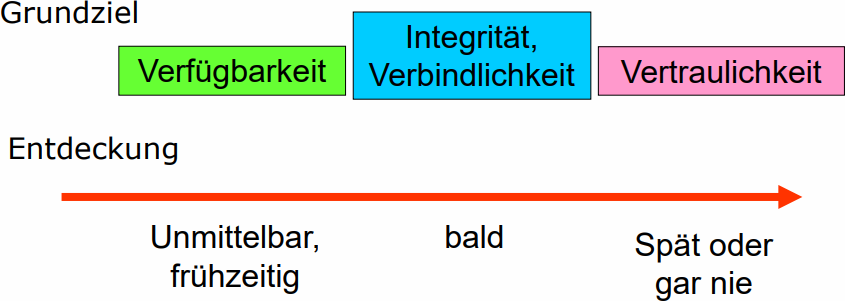
\includegraphics[width=16cm]{images/grundziel-entdeckung.png}
    \caption{Zeitpunkt der Entdeckung eines Grundziel-Verlustes}
    \label{grundziel-entdeckung}
    \end{center}
\end{figure}

\paragraph*{Erklären Sie die Zusammenhänge zwischen Risiko, Sicherheit, Eintretenshäufigkeit, Schadenshöhe, Restrisiko?}
\begin{itemize}[noitemsep,topsep=0pt,leftmargin=*]
    \item Risiko: Gefahr, Problem welches entstehen kann.\index{Risiko}
    \item Sicherheit: Schutz vor Risiko\index{Sicherheit}
    \item Eintretenshäufigkeit: Wahrscheinlichkeit, dass Risiko eintritt\index{Eintretenshäufigkeit}
    \item Restrisiko: Sicherheit deckt einen Teil des Risikos ab, jedoch nur gewisses Budget, somit bleibt Restrisiko, z.B. Erdbeben in San~Francisco oder Istanbul\index{Restrisiko}
\end{itemize}

\paragraph*{Zusammenhang}Durch Sicherheitsmassnahmen kann man die Eintretenshäufigkeit von einem Risiko mindern und somit auch den Schaden reduzieren, zusätzlich wird auch das Restrisiko kleiner oder kann sogar ausgeschlossen werden.

\paragraph*{Was ist eine Risikoanalyse? Wozu dient sie?}\index{Risikoanalyse}
\begin{enumerate}[noitemsep,topsep=0pt,leftmargin=*]
    \item Risiken zu erkennen
    \item Risiken analysieren
    \item Risikobewertung
    \item Nächster Schritt wäre das Risiko zu mindern mit den Erkenntnissen aus den ersten 3 Punkten.
    \item Massnahmen ergreifen und umsetzen.
\end{enumerate}

\paragraph*{Welche Möglichkeiten zur Behandlung (\flqq Mitigation\footnote{Verminderung} \frqq) stehen zur Verfügung? Ordnen Sie diese in der Reihenfolge, wie man sie typischerweise anwendet. Geben Sie ein kurzes Beispiel oder eine Erläuterung}
\begin{itemize}[noitemsep,topsep=0pt,leftmargin=*]
    \item Priorisieren: welches Risiko muss ich zuerst behandeln
    \item Vermindern: Massnahmen ergreifen, um Eintretenshäufigkeit und Schadensausmass zu vermindern
    \item Vermeiden: Massnahmen oder Wege einleiten um das Risiko auszuschliessen
    \item Akzeptieren: Ähnlich wie Ignorieren und das Risiko einfach hinnehmen
\end{itemize}

\paragraph*{Welche Gefährdungen und Bedrohungen kennen Sie? Gliedern Sie diese in verschiedene Kategorien.}\index{Gefährdungen}\index{Bedrohungen}
\begin{itemize}[noitemsep,topsep=0pt,leftmargin=*]
    \item Bruteforce, Phishing, DDoS, Injections, Spoofing, frustrierte Mitarbeiter, Anonymous, NSA, Naturgewalt, Hacker, Wirtschaftsspionage etc.
\end{itemize}

\subsubsection*{Stellen Sie Wissen – Information – Daten in eine Beziehung. Worauf bezieht sich die IT-Sicherheit? Was verstehen Sie unter integraler\footnote{Die Integrale Sicherheit überprüft Personen und Unternehmen mit Zugang zu vertraulichen oder geheimen Informationen, Materialien oder Anlagen. - https://www.sbis.ch} / holistischer\footnote{ganzheitlich} Sicherheit?}\index{Wissen}\index{Information}\index{Daten}
Ziel ist das grösste Niveau der Sicherheit zu erzielen (Gesamtsystem) wichtig ist wie sich die einzelnen Sicherheitskomponenten ergänzen und zusammenspielen. (Siehe Abbildung \ref{Wissenspyramide})
\begin{itemize}[noitemsep,topsep=0pt,leftmargin=*]
    \item \textbf{Informationssicherheit:}\index{Informationssicherheit} Schutz der Information als solche, Medien unabhängig Elektronischer Datenträger
    \item \textbf{IT-Sicherheit:}\index{IT-Sicherheit} Schutz der Informationen in ICT-Systemen. (Server/Host)
    \item \textbf{Integrale Sicherheit vs. holistische Sicherheit:}\index{Integrale Sicherheit}\index{Holistische Sicherheit} Umfassende Betrachtung aller Sicherheitsaspekte einer Organisation.
\end{itemize}

\subsubsection*{Bedeutung des Managements / GL im Rahmen von AKVs}
Ohne Management-Support geht gar nichts\footnote{Aufgaben, Kompetenzen und Verantwortlichkeiten}.
\begin{itemize}[noitemsep,topsep=0pt,leftmargin=*]
    \item Keine Ressourcen (Zeit und Geld)
    \item Keine Kompetenzen (Befehls-und Umsetzungsgewalt)
    \item Keine Priorität
    \item Das Management trägt die Risiken (Haftung für Mitarbeiter etc.) und entscheidet über die eingesetzten Ressourcen
    \item Häufig fehlendes Know-How der Managementetage
\end{itemize}

\paragraph*{Wie gehen Sie konkret vor, um die Informationssicherheit einzuführen?}\index{Informationssicherheit}
\begin{itemize}[noitemsep,topsep=0pt,leftmargin=*]
    \item Management ins Boot holen
    \item Prozess der Informationssicherheit etablieren (Know-How vermitteln oder zumindest das Thema greifbar machen für Management)
    \item Verantwortlichkeiten festlegen
    \item Sicherheit allumfassend betrachten
    \item Schrittweise und stetig umsetzen (kontinuierlicher Prozess)
\end{itemize}

\paragraph*{Begründen Sie, warum Informationssicherheit ein Prozess und kein Projekt sein muss.}\index{Informationssicherheit}
\begin{itemize}[noitemsep,topsep=0pt,leftmargin=*]
    \item Kontinuierliche Verbesserung der Sicherheit ein Muss
    \item Angriffe durch Hacker etc. entwickeln sich weiter, somit muss man immer auf dem neuesten Stand sein ("`up to date"' wie Dopingkontrollen im Sport)
    \item Projekt ist hingegen terminiert und irgendwann abgeschlossen
\end{itemize}

\paragraph*{Welche 3 Bereiche müssen Sie mit Ihren Massnahmen bespielen und warum?}\index{Massnahmen}
\begin{itemize}[noitemsep,topsep=0pt,leftmargin=*]
    \item Technik: kaufen und konfigurieren. Immer auf dem neuesten Stand und effizient eingesetzt.
    \item Prozesse: definieren, kontrollieren, weiterentwickeln. (Ist- und Soll-Prozess die ganze Zeit anpassen)
    \item Mitarbeiter: sensibilisieren und ausbilden. Meiner Ansicht nach auch Motivation und Loyalität fördern. (Interesse des Mitarbeiters wecken)
\end{itemize}

\paragraph*{Beschreiben Sie den Zweck von Datenschutz? Recherchieren Sie den heutigen Stand CH und die Veränderung durch die EU-DSGVO}\index{Datenschutz}
\paragraph*{TODO}

\paragraph*{Setzen Sie die Begriffe Zutritt, Zugang und Zugriff in Beziehung.}{Siehe \underline{\nameref{sec:Grundbegriffe}}, Seite \pageref{sec:Grundbegriffe}}


%%%%%%%%%%
\part{Kryptographie (SW~02-04)}
\section{Symmetrische Kryptographie}
\subsection*{Sie verstehen was Steganographie ist}
\paragraph*{Steganographie}\index{Steganographie}Verstecken von Information, z.B. in Bildern oder Audiofiles. \underline{\href{https://www.petitcolas.net/steganography/index.html}{Siehe Link}}\footnote{https://www.petitcolas.net/steganography/index.html}


\subsection*{Sie verstehen was Private-Key-Kryptographie ist, welche Arten von Sicherheit es gibt und welche Angriffsarten auf Verschlüsselung existieren}\index{Private-Key-Kryptographie}
\paragraph*{Zeichencodierung}Kodierung (\textsl{Encoding}) heisst, einen Wert mit Symbolen eines Zeichensatzes darzustellen. Beispiel:\newline %bleibt
\begin{tabular}{|ll|}
    \hline
        Dezimalsystem & 100\\
        Binärsystem & 1100100\\
        Hexadezimalsystem (`hex') & 64\\
        ASCII & hello\\
        Base64 & aGVsbG8=\\
    \hline
\end{tabular}
{\color{red}\textbf{Achtung: Kodierung $\neq$ Verschlüsselung}}

\paragraph*{Symmetrische Verschlüsselung}Bei symmetrischen Verschlüsselungsverfahren gibt es im Gegensatz zu den asymmetrischen Verfahren, \textbf{nur einen einzigen Schlüssel}. Dieser Schlüssel ist für die Verschlüsselung, als auch für die Entschlüsselung zuständig.\index{Symmetrische Kryptographie}

\paragraph*{Secret Key Verschlüsselung}Secret Key (`Symmetrische') Verschlüsselung wird zwischen zwei Parteien verwendet, welche einen \textbf{gemeinsamen Schlüssel} besitzen. Ausserdem wird sie oft verwendet, wenn der gleiche Benutzer ein Dokument verschlüsseln und zu einem späteren Zeitpunkt wieder entschlüsseln muss.\index{Secret Key}
\begin{figure}[ht]
    \begin{center}
    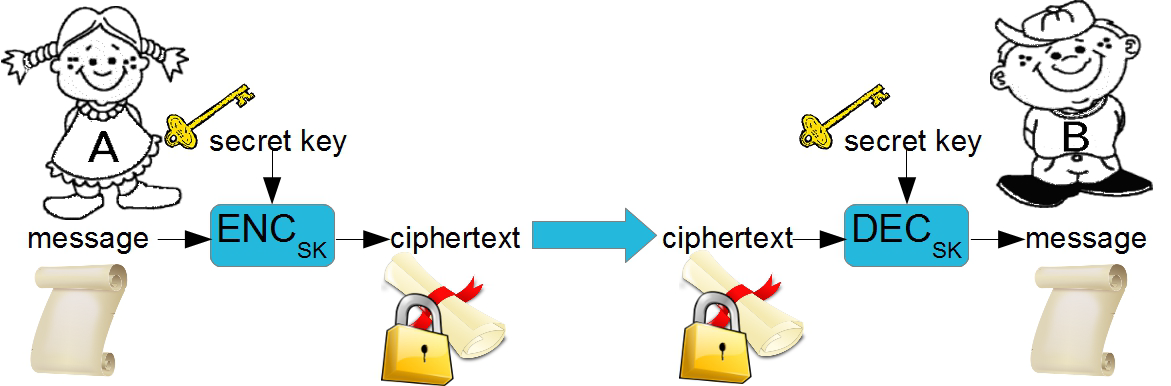
\includegraphics[width=14cm]{images/secretkey.png}
    \caption{Alice verschlüsselt, Bob entschlüsselt mit dem gemeinsamen Schlüssel}
    \label{secretkey}
    \end{center}
\end{figure}

\paragraph*{Secret Key Verschlüsselung: Algorithmen}Beispiele für symmetrische Verschlüsselung \newline
\begin{tabular}{|c|c|c|c|c|}
    \hline
    Name&Blocklänge&Schlüssellänge&Jahr&Kommentar\\
    \hline
    DES&64 Bit&56 Bit&1970&gebrochen\\
    Triple DES&64 Bit&112 Bit ($3\times56$ Bit)&  &nicht mehr empfohlen\\
    RC4&stream cipher&8-2040&1987&gebrochen\\
    IDEA&64 Bit&128 Bit&1990&nicht mehr empfohlen\\
    RC5&64 oder 128 Bit&4-256 Bit&1994&nicht mehr empfohlen\\
    Camellia&128 Bit&128, 192 oder 256 Bit&2000& \\
    Twofish&128 Bit&128, 192 oder 256 Bit&1998& \\
    AES (Rijndal)&128 Bit&128, 192 oder 256 Bit&2000& \\
    \hline
\end{tabular}

\paragraph*{Informationstheoretische Sicherheit}Das Ziel informationstheoretischer Sicherheit ist der Schutz von Daten vor unbefugtem Zugriff während der Übertragung. Im Unterschied zur Kryptographie basiert informationstheoretische Sicherheit nicht auf der Annahme, dass die Rechenleistung eines unberechtigten Empfängers nicht gross genug ist, um die Daten zu decodieren. Vielmehr garantiert informationstheoretische Sicherheit, dass ein unberechtigter Empfänger selbst bei beliebig grosser Rechenleistung nicht in der Lage ist, solcherart geschützte Nachrichten zu decodieren. Mit anderen Worten erhält ein Angreifer durch den Geheimtext keinerlei (zusätzliche) Information über den Klartext\cite{renner2006}.\index{Informationstheoretische Sicherheit}
 Beispielsweise ist OTP informationstheoretisch sicher. \newline %bleibt
Formal:
\begin{math}
    P(M=m) = P(M=m|C=c)
\end{math} {\color{red}Erklärung der Variablen??}

\paragraph*{Berechenmässige Sicherheit}\index{Berechenmässige Sicherheit}\label{para:Berechenmässige Sicherheit}Der sicheren Übertragung und Aufbewahrung vertraulicher Daten kommt in unserer von Information dominierten Gesellschaft immer grössere Bedeutung zu. Die heute gebräuchlichen Verfahren zur Datenverschlüsselung bieten allerdings nur beschränkte, sogenannt berechenmässige Sicherheit. Das bedeutet, dass diese prinzipiell von einem Angreifer, der über genügend Rechenleistung (zum Beispiel einen, heute noch hypothetischen, Quantencomputer) verfügt, gebrochen werden können\cite{renner2006}.

\paragraph*{Kerckhoff's Prinzip}\index{Kerckhoff's Prinzip}\label{para:Kerckhoff's Prinzip}Der Angreifer kennt den Algorithmus und alle Details des Systems. Nur der Schlüssel ist geheim.

\paragraph*{Angriffsarten}Bei der Sicherheit von modernen Verschlüsselungssystemen wird zwischen den Angriffs-möglichkeiten des Angreifers unterschieden:
\begin{itemize}[noitemsep,topsep=0pt,leftmargin=*]
    \item \textbf{Ciphertext only attack:} Angreifer erhält nur den zu entschlüsselnden Geheimtext
    \begin{figure}[ht]
        \begin{center}
        \includegraphics[width=8cm]{images/coa.png}
        \caption{Nur Geheimtext}
        \label{coa}
        \end{center}
    \end{figure}\index{Ciphertext only attack}
    \item \textbf{Known plaintext attack:} Angreifer erhält zusätzlich andere Klartext-Geheimtext-Paare
    \begin{figure}[ht]
        \begin{center}
        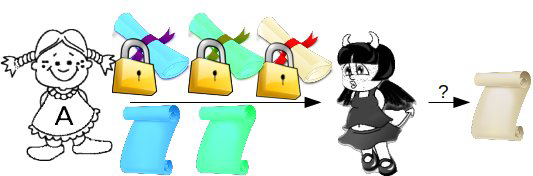
\includegraphics[width=8cm]{images/kpa.png}
        \caption{Klartext-Geheimtext-Paare}
        \label{kpa}
        \end{center}
    \end{figure}\index{Known plaintext attack}
    \item \textbf{Chosen plaintext attack:} Angreifer kann zusätzliche Klartexte wählen, zu denen er auch die Geheimtexte erhält
    \begin{figure}[ht]
        \begin{center}
        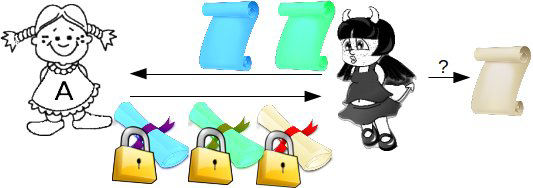
\includegraphics[width=8cm]{images/cpa.png}
        \caption{Klartexte und Geheimtexte}
        \label{cpa}
        \end{center}
    \end{figure}\index{Chosen plaintext attack}
\end{itemize}


\subsection*{Sie können "`klassische"' symmetrische Verschlüsselungverfahren wie Caesar cipher, Vigenère cipher, one-time pad anwenden und verstehen die Vor- und Nachteile bzw. Schwachstellen dieser Verfahren}\index{Klassische symmetrische Verschlüsselungsverfahren}

\paragraph*{Caesar cipher}\index{Caesar cipher}\label{para:Caesar cipher}Caesar-Verschlüsselung ist ein einfaches symmetrisches Verschlüsselungsverfahren, das auf der monographischen und monoalphabetischen Substitution basiert.\\
\textbf{Vorteil:} es ist \textbf{einfach}.\\
\textbf{Nachteil:} es ist \textbf{unsicher}, da es sehr schnell geknackt werden kann.\\
\textbf{Schwachstelle:} Die in der natürlichen Sprache ungleiche Verteilung der Buchstaben wird durch diese Art der Verschlüsselung nicht verborgen, so dass eine Häufigkeitsanalyse (Frequenzanalyse) das Wirken einer einfachen monoalphabetischen Substitution enthüllt.

\paragraph*{Caesar cipher: Vorgang}
\begin{itemize}[noitemsep,topsep=0pt,leftmargin=*]
    \item Verschiebt jeden Buchstaben des Alphabets um eine bestimmte Anzahl Stellen
    \item Soll bereits von Julius Caesar verwendet worden sein, daher der Name
    \item Der Schlüssel wird entweder als Anzahl Stellen, um die verschoben wird, oder als Buchstaben, auf den `A' verschoben wird angegeben
    \item Variante: ROT13 (Verschlüsselung = Entschlüsselung)
    \item Problem 1: Schlüssellänge (nur 26 verschiedene Schlüssel)
    \item Problem 2: Frequenzanalyse
\end{itemize}
\begin{figure}[H]
    \begin{center}
    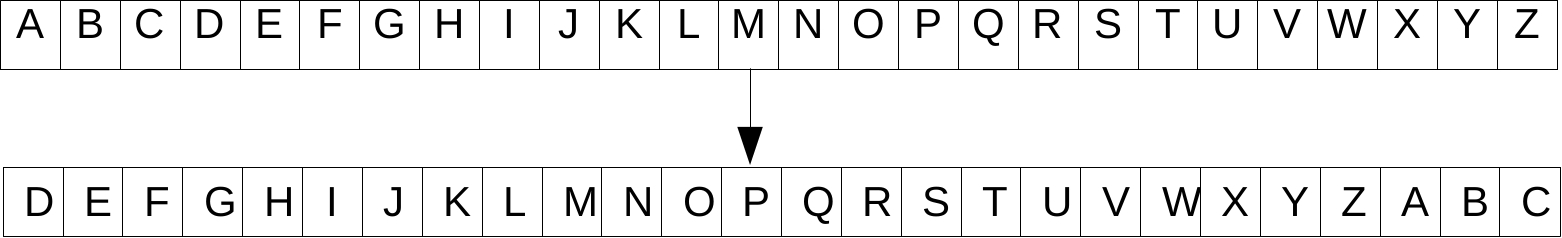
\includegraphics[width=12cm]{images/caesar.png}
    \caption{Caesar cipher mit Verschiebung um 3 Stellen}
    \label{caesar}
    \end{center}
\end{figure}

\noindent
Das folgende Diagramm zeigt die Häufigkeitsverteilung der Buchstaben in einem längeren Text in deutscher Sprache:
\begin{figure}[H]
    \begin{center}
    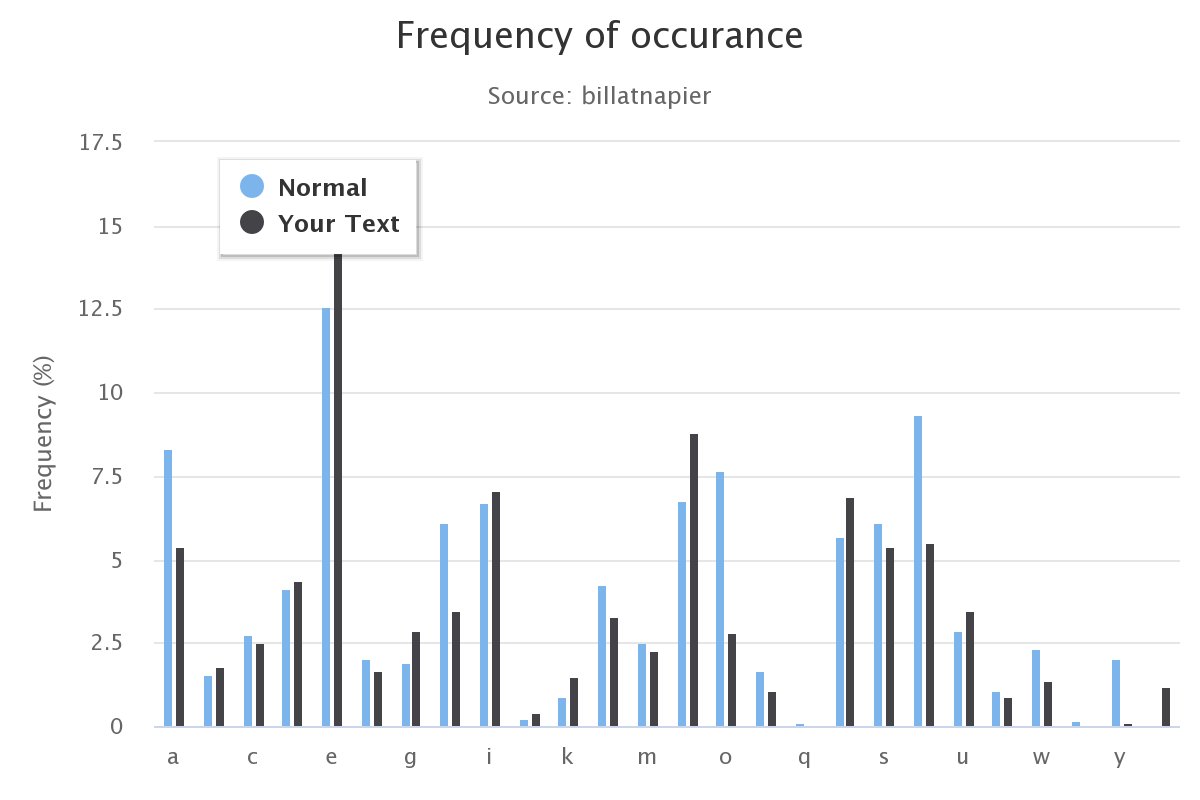
\includegraphics[width=10cm]{images/frequency0.png}
    \caption{Frequenzanalyse unchiffriert}
    \label{frequencynormal}
    \end{center}
\end{figure}

\noindent
Wie zu erwarten, ist der häufigste Buchstabe E, gefolgt von N und I, wie es im Deutschen üblicherweise der Fall ist. Wird der Text mit dem Schlüssel 10 (oder anders gesagt, mit dem Schlüsselbuchstaben J) chiffriert, erhält man einen Geheimtext, der folgende Häufigkeitsverteilung besitzt:
\begin{figure}[H]
    \begin{center}
    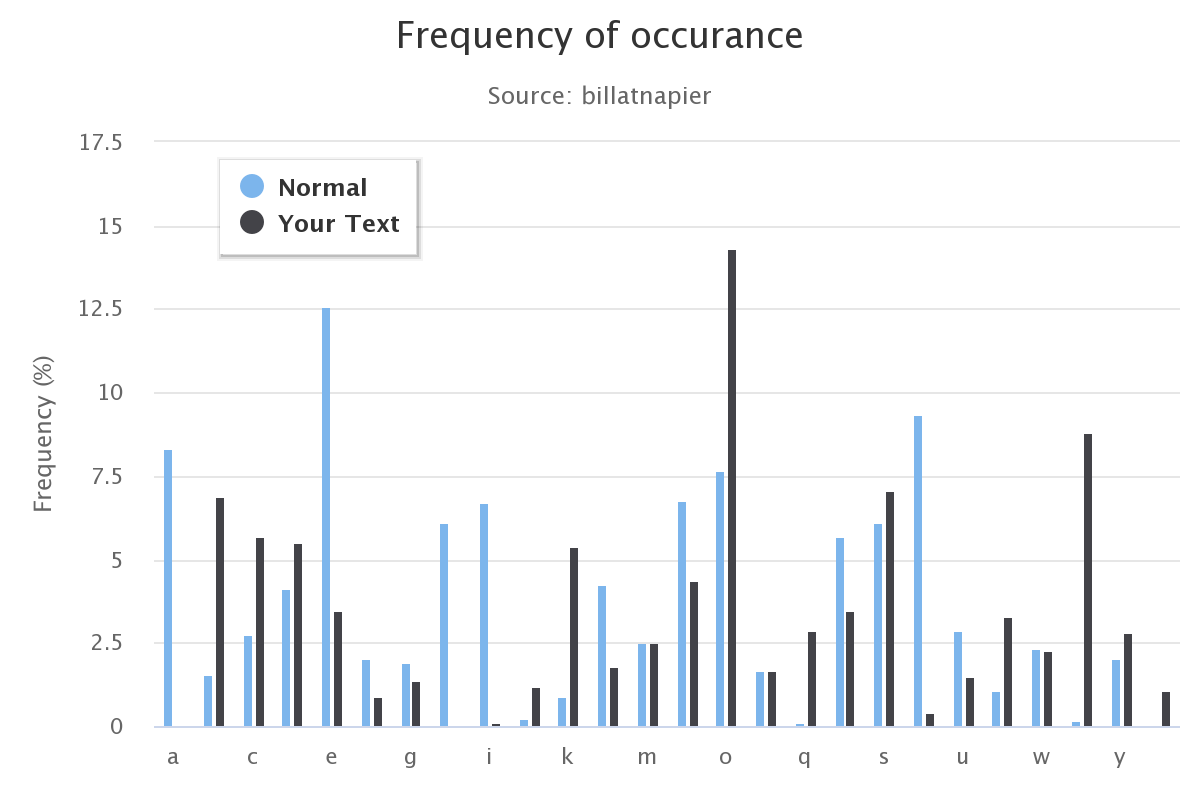
\includegraphics[width=10cm]{images/frequency1.png}
    \caption{Frequenz um 10 Stellen verschoben}
    \label{frequencycaesar}
    \end{center}
\end{figure}

\noindent
Der häufigste Buchstabe ist hier O, gefolgt von X und S. Man erkennt auf den ersten Blick die Verschiebung des deutschen "`Häufigkeitsgebirges"' um zehn Stellen nach hinten und besitzt damit den Schlüssel. Voraussetzung ist lediglich, dass man die Verteilung der Zeichen des Urtextes vorhersagen kann.

\noindent
Besitzt man diese Information nicht oder möchte man auf die Häufigkeitsanalyse verzichten, kann man auch die Tatsache ausnutzen, dass bei der Cäsar-Chiffre nur eine sehr kleine Anzahl möglicher Schlüssel in Frage kommt. Da die Grösse des Schlüsselraums nur 25 beträgt, was einer "`Schlüssellänge"' von nicht einmal 5~bit entspricht, liegt nach Ausprobieren spätestens nach dem 25. Versuch der Klartext vor.

\paragraph*{Vigenère cipher}\index{Vigenère cipher}\label{para:Vigenère cipher}
\begin{itemize}[noitemsep,topsep=0pt,leftmargin=*]
    \item Schlüssel: Wort der Länge $L$
    \item Jeder Buchstabe im Text wird mit der Caesar cipher des entsprechenden Schlüsselwortes verschlüsselt
    \item Anzahl mögliche Schlüssel: $26^L$
    \item Problem: Frequenzanalyse jeder $L$'ten Stelle
\end{itemize}
\begin{figure}[H]
    \begin{center}
    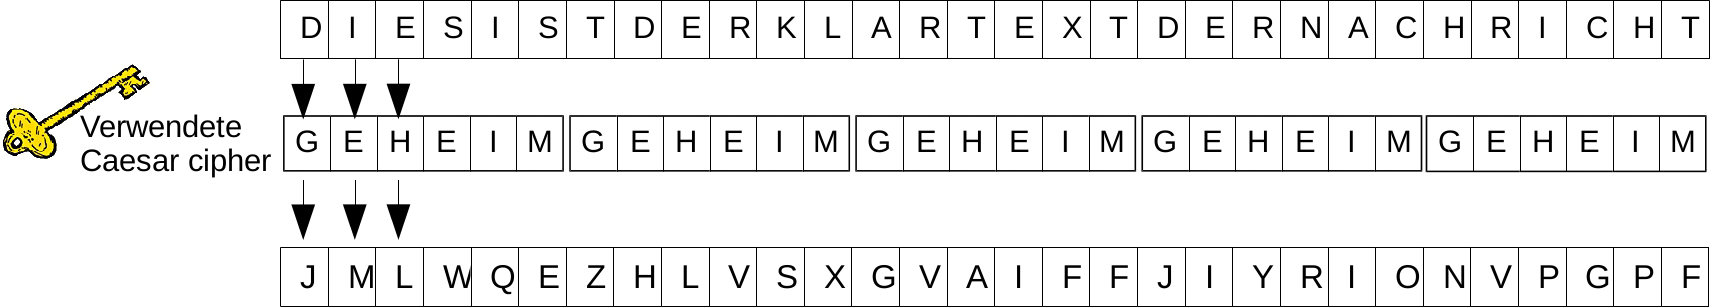
\includegraphics[width=16cm]{images/vigenere.png}
    \caption{Vigenère cipher}
    \label{vigenere}
    \end{center}
\end{figure}

\paragraph*{One-time pad}\index{One-time pad}\label{One-Time Pad}
\begin{itemize}[noitemsep,topsep=0pt,leftmargin=*]
    \item Jede Stelle wird mit einem anderen Schlüssel verschlüsselt
    \item Darf nur 1 Mal verwendet werden!
    \item Anzahl möglicher Schlüssel = Anzahl möglicher Nachrichten
    \item Ist sicher, d.h. Geheimtext verrät keinerlei (zusätzliche) Information über den Klartext
    \item Intuitiv: Für einen bestimmten Geheimtext sind \textbf{alle} Klartexte (dieser Länge) möglich
\end{itemize}
\begin{figure}[H]
    \begin{center}
    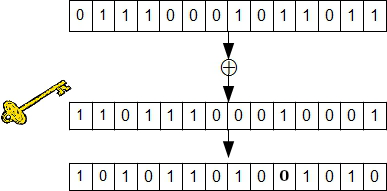
\includegraphics[width=12cm]{images/otp.png}
    \caption{Funktionsweise des OTP}
    \label{otp}
    \end{center}
\end{figure}


\subsection*{Sie wissen welche modernen Verschlüsselungsalgorithmen in der Praxis verwendet werden und was deren Eigenschaften sind}
\paragraph*{TODO}


\subsection*{Sie verstehen was eine Hashfunktion ist und welche Eigenschaften eine kryptographische Hashfunktion ausmachen, bzw. was es heisst, wenn eine Hashfunktion gebrochen ist}

\paragraph*{Hashfunktion}\index{Hashfunktion}\label{para:Hashfunktion}Eine Hashfunktion ist eine Abbildung, die eine grosse Eingabemenge (die Schlüssel) auf eine kleinere Zielmenge (die Hashwerte) abbildet. Die Eingabemenge kann Elemente unterschiedlicher Längen enthalten, die Elemente der Zielmenge haben dagegen meist eine feste Länge.
\begin{figure}[H]
    \begin{center}
    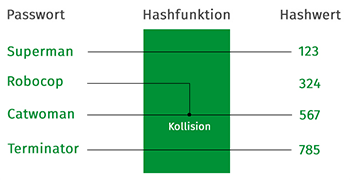
\includegraphics[width=8cm]{images/hash1.png}
    \caption{Einfaches Beispiel einer Hashfunktion}
    \label{hash1}
    \end{center}
\end{figure}

\noindent
Auf der linken Seite sehen wir 4 Passwörter von beispielsweise 4 Mitarbeitern eines Unternehmens. Die Hashfunktion  wandelt nun diese Passwörter in eine Zeichenfolge (dem Hashwert) mit einer festen Länge (hier 3 Zeichen) um. Für das Passwort "`Superman"' bekommt man den Hashwert 123, dem Passwort "`Robocop"' wird de Hashwert 567 zugeordnet, genauso wie dem Passwort "`Catwoman"' und "`Terminator"' bekommt 785.
Hashfunktionen reduzieren zunächst nur Zeichen beliebiger Länge (unterschiedliche Passwörter) auf Zeichen fester Länge (im Beispiel 3 Zeichen). Sie werden also in eine kleine, kompakte Form gebracht.

\paragraph*{Zusatzinfo zum Hashwert}Der Hashwert ist das Ergebnis, das mittels einer Hashfunktion berechnet wurde. Man definiert eine feste Länge, wie lang ein Hashwert immer sein darf. Oft wird der Hashwert als eine hexadezimale Zeichenkette codiert, d.h. der Hashwert besteht aus einer Kombination von Zahlen und Buchstaben zwischen 0 und 9 sowie A bis F (als Ersatz für die Zahlen 10 bis 15). Ein Hashwert aus 10 hexadezimalen Zeichen könnte so aussehen: "`3d180ab86e"'.

\paragraph*{Eigenschaft einer Hashfunktion}
\begin{itemize}[noitemsep,topsep=0pt,leftmargin=*]
    \item Einwegfunktion: Aus dem Hashwert darf nicht der originale Inhalt erzeugt werden können. In unserem Beispiel darf es nicht möglich sein, aus dem Hashwert "`123"' den Ursprungstext "`Superman"' zu erzeugen.
    \item Kollisionssicherheit: Den unterschiedlichen Texten darf nicht derselbe Hashwert zugeordnet sein. Ist diese Voraussetzung erfüllt, so spricht man auch von \textbf{kryptographischen Hashfunktionen}. In unserem Beispiel liegt eine Kollision vor, da die Passwörter "`Robocop"' und "`Catwoman"' denselben Hashwert haben. Damit ist die Hashfunktion im Bild nicht kollisionssicher und es handelt sich nicht um eine kryptografische Hashfunktion.
    \item Schnelligkeit: Das Verfahren zu Berechnung des Hashwertes muss schnell sein.
\end{itemize}

\paragraph*{Algorithmen für Passwortspeicherung}\index{Passwort}\index{Password Based Key Derivation Functions}Um Passwörter zu speichern werden sog. \textbf{Password Based Key Derivation Functions (PBKDF)} verwendet, d.h. \textbf{kryptographische Hashfunktionen} welche zusätzlich resourcen-intensiv (langsam) zu berechnen sind.
\begin{itemize}[noitemsep,topsep=0pt,leftmargin=*]
    \item basieren auf einer herkömmlichen Hashfunktion, welche mehrmals verknüpft ausgeführt wird
    \item die Geschwindigkeit wird durch einen Parameter bestimmt, welcher die Anzahl Runden angibt
    \item damit werden Angriffe mittels speziell für die Berechnung von Hashfunktionen optimierte Hard- und Software erschwert
\end{itemize}
Beispiele sind PBKDF2\index{PBKDF2} und bcrypt\index{bcrypt} (Blowfish-Algorithmus), welche zusätzlich viel Memory benötigen, oder scrypt\index{scrypt} (Entwicklung motiviert durch Verwundbarkeit von PBKDF2 und bcrypt durch Brute-Force-Attacken) und Argon2\index{Argon2}.

\paragraph*{Gebrochene Hashfunktionen}"`Gebrochen"' = "`geknackt"'. Dies war z.B. bei LinkedIn und Dropbox der Fall. Wie können aber Passwörter geknackt werden, wenn man wegen der Einweg-Eigenschaften der Hashfunktionen nicht auf den ursprünglichen Text zurückschliessen kann?
Zunächst muss man wissen, dass fast alle Algorithmen "`offen"' liegen, diese also auch von Angreifern genutzt werden können. Das hat zur Folge, dass der Hashwert von einem Passwort immer gleich ist, egal ob es die Plattform oder der Angreifer berechnet.
Passwort "`Superman” = MD5-Hash: "`527d60cd4715db174ad56cda34ab2dce"'.
Ein Angreifer kann sich also eine Liste mit typischen unsicheren Passwörtern erstellen und es durch den Hashgenerator jagen. Wenn er nun die Datenbank mit den Hashwerten der Plattform stiehlt, kann er die Hashwerte mit seiner Liste vergleichen. Findet er in der geklauten Liste den Hashwert "`527d60cd4715db174ad56cda34ab2dce"', so weiss er, dass dieser Hashwert dem Passwort "`Superman"' zugeordnet ist. Solche Listen nennt man \textbf{rainbow tables}.

\paragraph*{Hashfunktionen}\index{Hash-Algorithmen}Algorithmen\newline %bleibt
\begin{tabular}{|c|c|c|c|}
    \hline
    Name&Block Länge&Output Länge&Bemerkung\\
    \hline
    MD5&512&128&gebrochen\\
    SHA-1&512&160&gebrochen\\
    SHA-256&512&256& \\
    SHA-384&1024&384& \\
    SHA-512&1024&512& \\
    SHA3-256&1088&256& \\
    SHA3-384&832&384& \\
    SHA3-512&576&512& \\
    \hline
\end{tabular}


\subsection*{Sie kennen moderne Hashfunktionen und wissen welche Eigenschaften diese haben}
\paragraph*{TODO}


\subsection*{Sie kennen Anwendungen von Hashfunktionen}
Verwendung von Hashfunktionen
\begin{itemize}[noitemsep,topsep=0pt,leftmargin=*]
    \item Identifikation einer Datei in peer-to-peer Netzwerken
    \item Fehlererkennung
    \item Integritätsprüfung
    \begin{itemize}[noitemsep,topsep=0pt,leftmargin=*]
        \item Symmetric Key Solution: Message Authentication Code (MAC) durch einen `keyed hash'
        \item Asymmetic Key Solution: Digital Signature durch Signatur des Hashwertes
    \end{itemize}
    \item "`Proof of work"' in Blockchain
\end{itemize}


\subsection*{Sie wissen was ein keyed Hash (HMAC) ist und wofür dieser verwendet werden kann}

\paragraph*{HMAC}Ein Keyed-Hash Message Authentication Code (HMAC) ist ein Message Authentication Code (MAC), dessen Konstruktion auf einer kryptografischen Hash-Funktion, wie z.B. MD5 und einem geheimen Schlüssel basiert.



\subsection*{Sie kennen die "`Best-practices"' zu Passwortsicherheit und wissen, gegen welche Angriffe diese schützen}
\paragraph*{Passwortsicherheit}Best practices
\begin{itemize}[noitemsep,topsep=0pt,leftmargin=*]
    \item Gespeichert wird nur der \textbf{Hashwert} des Passwortes
    \item Ziel: Admin oder Angreifer mit Zugang zur DB erhalten das Passwort nicht
\end{itemize}
Oder noch besser:
\begin{itemize}[noitemsep,topsep=0pt,leftmargin=*]
     \item Das Passwort wird gemeinsam mit einem \textbf{Salt} gehasht. Dieser neue Hash wird in der DB abgelegt. Der Salt muss nicht geheim, aber einzigartig (\textsl{unique}) sein.
    \item Ziel: Aufgrund der einzigartigen DB-Einträge ist nicht erkennbar, ob zwei Benutzer dasselbe Passwort haben. Zusätzlich kann ein Angreifer nicht die häufigsten Passwörter hashen und danach vergleichen, welcher Benutzer in der DB dieses Passwort verwendet hat. Er muss jeden Eintrag einzeln angreifen.
    \item Als Hashfunktion wird eine langsame und resourcen-intensive Hashfunktion verwendet, z.B. scrypt.
    \item Ziel: Verlangsamen einer Offline-Attacke auf die Passwort-Hashes.
\end{itemize}

\subsection*{Kontrollfragen SW 02}
\paragraph*{Wie hängt die Schlüssellänge eines Verschlüsselungsalgorithmus mit dessen Sicherheit
zusammen?}\index{Schlüssellänge}Die Schlüssellänge ist ein wichtiger Parameter von symmetrischen oder asymmetrischen Verschlüsselungsverfahren. Sie gibt Auskunft darüber, wie viele unterschiedliche Schlüsselwerte ein Schlüssel bei einem bestimmten Verfahren annehmen kann.\\
Da oft der einzige Weg einen Schlüssel zu "`knacken"' darin besteht, über eine sogenannte Brut-Force-Attacke alle sich bietenden Möglichkeiten auszuprobieren, bestimmt die Schlüssellänge die hierfür aufzuwendende Rechenleistung und Rechenzeit.\index{Brute-Force}

\paragraph*{Was besagt das Kerckhoff-Prinzip?}{Siehe \underline{\nameref{para:Kerckhoff's Prinzip}}, Seite \pageref{para:Kerckhoff's Prinzip}}

\paragraph*{Was ist berechenmässige Sicherheit?}{Siehe \underline{\nameref{para:Berechenmässige Sicherheit}}, Seite \pageref{para:Berechenmässige Sicherheit}}

\paragraph*{Welche Eigenschaft einer kryptographischen Hashfunkton muss beim "`Bitcoin mining"' gebrochen werden?} Bitcoin verwendet Hashfunktionen auf zwei Weisen:
\begin{enumerate}[noitemsep,topsep=0pt,leftmargin=*]
    \item Miner müssen Hashes mit SHA256 berechnen, um Blöcke zu finden
    \item Der öffentliche Schlüssel des Signatur-Algorithmus wird sowohl mit SHA256 als auch RIPEMD-160 gehasht, um die Adresse zu bilden
\end{enumerate}{Für weitere Infos siehe \underline{\nameref{para:Hashfunktion}}, Seite \pageref{para:Hashfunktion}}


\section{Asymmetrische Kryptographie}
\paragraph*{Asymmetrische Verschlüsselung}In der asymmetrischen Kryptographie (Verschlüsselung) arbeitet man nicht mit einem einzigen Schlüssel, sondern mit einem \textbf{Schlüsselpaar}. Bestehend aus einem \textbf{öffentlichen} und einem \textbf{privaten Schlüssel}. Man bezeichnet diese Verfahren als asymmetrische Verfahren oder \mbox{Public-Key-Verfahren}.

\subsection*{Sie verstehen was Public-Key-Kryptographie ist, worauf deren Sicherheit basiert und wie sie zur Verschlüsselung, für Signaturen und zur Authentisierung verwendet werden kann}

\paragraph*{Public Key Verschlüsselung}Basiert auf Funktionen, welche einfach zu berechnen sind, deren Umkehrfunktion aber (vermutlich) schwierig zu berechnen ist.
Beispiel:\newline %bleibt
\noindent
\begin{tabular}{|ll|}
    \hline
    Multiplikation (einfach):&$97\times84=8051$\\
    Faktorisieren (schwierig):&$8051=?$\\
    \hline
\end{tabular}

\paragraph*{TODO}BILDER aus "`The Science of Secrecy"'
\subsection*{Sie kennen die gängigen asymmetrischen Verschlüsselungs- und Signaturalgorithmen und wissen, worauf deren Sicherheit basiert}
\paragraph*{TODO}


\subsection*{Sie wissen wie Diffie-Hellmann-Schlüsselaustausch bzw. ElGamal-Verschlüsselung funktioniert}

\paragraph*{Diffie-Hellman (DH)}Diffie-Hellman ist ein Schlüsselvereinbarungsprotokoll. Der vereinbarte gemeinsame geheime Schlüssel kann danach zur Verschlüsselung der Nachricht verwendet werden.

\paragraph*{TODO}BILD \& ev. Beispiel Wiki

\paragraph*{ElGamal-Verschlüsselung}ElGamal verwendet DH um einen asymmetrischen Verschlüsselungsalgorithmus zu erstellen.

\paragraph*{TODO}BILD ElGamal

\paragraph*{TODO}ev. Beispielrechnung machen

\subsection*{Sie wissen was kryptographisch sichere Zufallszahlen sind und wo diese verwendet werden}

\paragraph*{TODO}

\subsection*{Sie wissen was eine elektronische Signatur ausmacht}

\paragraph*{Signatur}\index{Signatur}Die elektronische Signatur ist ein technisches Verfahren zur Überprüfung der Echtheit eines Dokuments, einer elektronischen Nachricht oder anderer elektronischer Daten sowie der Identität des Unterzeichnenden. Sie basiert auf einer Zertifizierungsinfrastruktur, die von vertrauenswürdigen Dritten verwaltet wird: den Anbieterinnen von Zertifizierungsdiensten. Die elektronische Signatur und die handschriftliche Unterschrift werden zudem mit dem neuen Gesetz unter bestimmten Bedingungen als gleichwertig betrachtet.
\begin{figure}[H]
    \begin{center}
    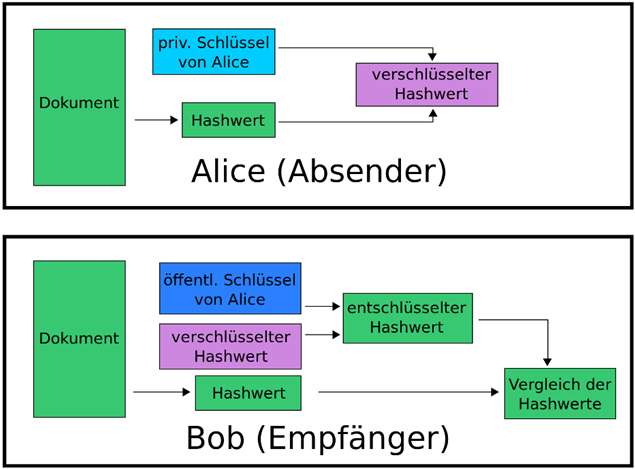
\includegraphics[width=12cm]{images/digisignatur1.png}
    \caption{Signatur im Detail}
    \label{digisig1}
    \end{center}
\end{figure}

\paragraph*{Beispiel}Max Meier erhält von seinem Kunden den Geschäftsvertrag – digital als PDF, wie es heutzutage üblich ist. Vergleichsweise altmodisch geht es aber nachher weiter: Meier druckt das Dokument aus und unterzeichnet es handschriftlich. Den unterschriebenen Vertrag steckt er schliesslich in einen Umschlag und wirft diesen in den nächstgelegenen Briefkasten. Viele Schritte für eine Unterschrift. Was Max Meier nicht weiss: Dokumente lassen sich auch digital unterzeichnen. Jede digitale Signatur basiert auf der sogenannten asymmetrischen Verschlüsselung. Sie wird auch als Public-Key-Verfahren bezeichnet und nutzt einen öffentlichen und einen privaten (geheimen) Schlüssel. Mit dem privaten Schlüssel wird die digitale Signatur erzeugt, während mit dem öffentlichen Schlüssel die Authentizität der Unterschrift überprüft wird.

\paragraph*{Eigenschaft einer Signatur}
\begin{enumerate}[noitemsep,topsep=0pt,leftmargin=*]
    \item \textbf{Fälschungssicherheit:} Nach dem Unterschreiben kann das Dokument nicht mehr (unerkannt) verändert werden.
    \item \textbf{Authentizität:} Die Unterschrift kann zweifelsfrei (überprüfbar) einer bestimmten Person zugeordnet werden.
    \item \textbf{Unleugbarkeit:} Der Unterzeichner kann später nicht abstreiten, das Dokument unterschrieben zu haben.
    \item \textbf{Willenserklärend:} Die Unterschrift kann nur willentlich (bewusst) unter das Dokument gesetzt worden sein.
\end{enumerate}
\begin{figure}[H]
    \begin{center}
    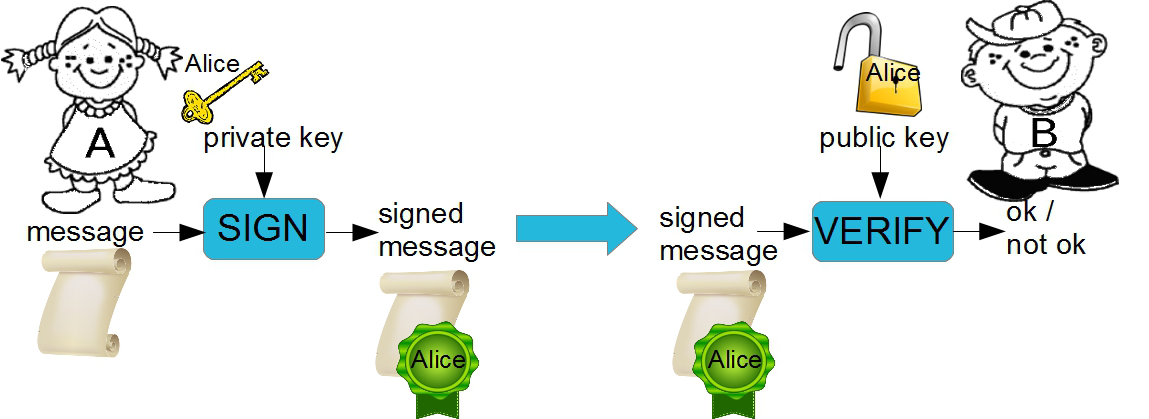
\includegraphics[width=12cm]{images/digisignatur0.png}
    \caption{Alice verschickt eine signierte Nachricht an Bob}
    \label{digisig0}
    \end{center}
\end{figure}


\subsection*{Sie wissen wie hybride Verschlüsselung bzw. hybride Signaturen funktionieren}
\paragraph*{Hybridverschlüsselung}\index{Hybridverschlüsselung}Eine Hybridverschlüsselung ist eine Kombination von symmetrischer und asymmetrischer Verschlüsselung. Dabei werden die Vorteile beider Verschlüsselungsverfahren genutzt. Symmetrische Verschlüsselung ist deutlich schneller, asymmetrische haben den Vorteil eines deutlich einfacheren Schlüsselaustausches. Der Ablauf ist folgendermassen:
\begin{itemize}[noitemsep,topsep=0pt,leftmargin=*]
    \item Sender Alice einen zufälligen symmetrischen Schlüssel, einen Session-Key
    \item Der Session-Key verschlüsselt die Daten/Nachricht symmetrisch
    \item Der Session-Key wird asymmetrisch mit Bob's Public-Key verschlüsselt
    \item Die verschlüsselten Sachen werden an Bob gesendet
    \item Bob entschlüsselt asymmetrisch den Session-Key mit seinem Private-Key
    \item Der Session-Key entschlüsselt nun die Nachricht symmetrisch
\end{itemize}
\begin{figure}[H]
    \begin{center}
    \includegraphics[width=12cm]{images/hybridverschlüsselung.png}
    \caption{Hybridverschlüsselung einer Nachricht}
    \label{hybrid}
    \end{center}
\end{figure}
Man erkennt schnell den Vorteil dieser Methode. Ein symmetrisches Verschlüsselungsverfahren ist sehr effizient auch im Verschlüsseln von grossen Datenmengen

\subsection*{Kontrollfragen SW 03}

\paragraph*{Vergleichen Sie symmetrische und asymmetrische Verschlüsselung bezüglich Anzahl Schlüssel, Schlüssellänge und Geschwindigkeit der Algorithmen}
\begin{itemize}[noitemsep,topsep=0pt,leftmargin=*]
    \item \textbf{Symmetrisch:} 1 Schlüssel, Schlüsselänge eher kürzer, Geschwindigkeit hoch
    \item \textbf{Asymmetrisch:} Mehrere Schlüssel (meistens 2), Schlüssellänge sehr sicher (lang), Geschwindigkeit tief
\end{itemize}

\paragraph*{Warum wird in der Praxis bei der Email-Verschlüsselung ein sog. hybrider Verschlüsselungsalgorithmus angewandt?}\index{Email-Verschlüsselung}\index{Hybrider Verschlüsselungsalgorithmus}Es muss schnell gehen und somit wird auf eine hybride Variante umgestiegen. Dies erhöht die Geschwindigkeit, ohne die Sicherheit zu mindern.


\section{Zertifikate und SSL-TLS}

\subsection*{Sie kennen die verschiedenen Arten von "`Trust"'}
Problematik: Wie ordnet man ein Public Key einer bestimmten Person / Entität zu?
\begin{figure}[H]
    \begin{center}
    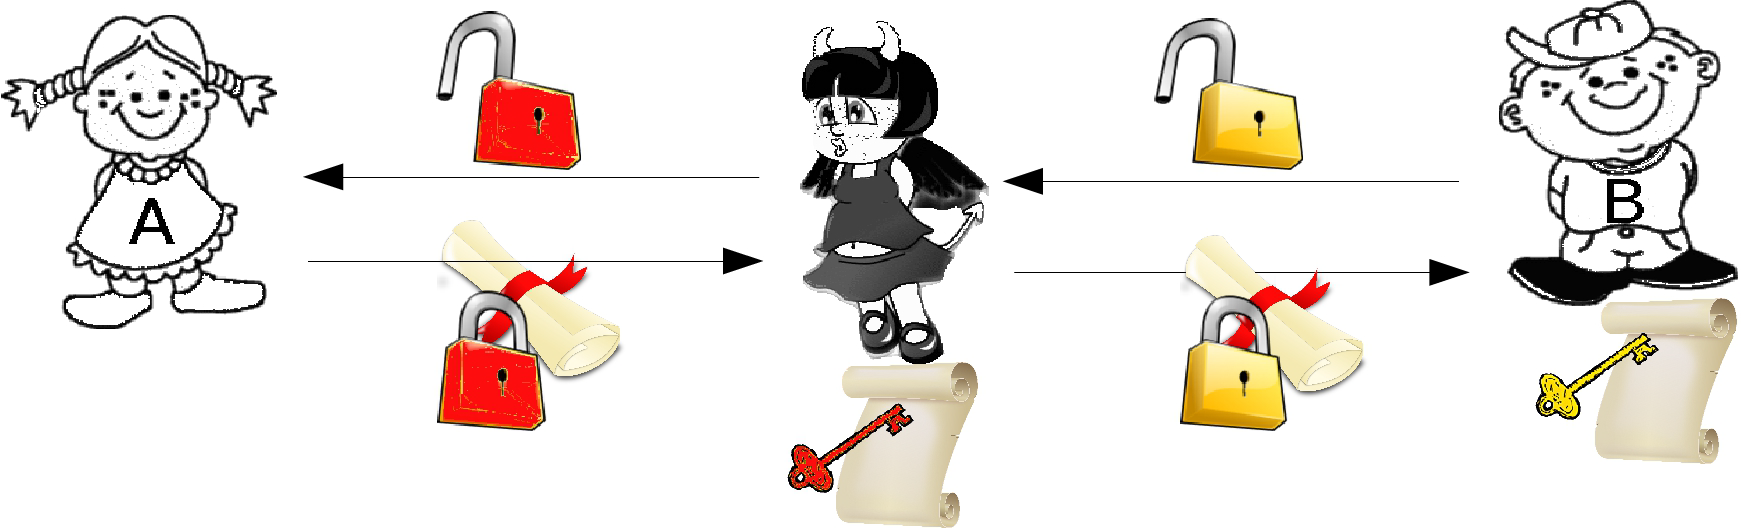
\includegraphics[width=14cm]{images/mitma.png}
    \caption{Eve als man in the middle}
    \label{mitma}
    \end{center}
\end{figure}

\paragraph*{Direct Trust}
Alice vertraut der Authentizität von Bob's Public Key, durch direktes Überprüfen, normalerweise über den Fingerprint des Key's.
\begin{figure}[H]
    \begin{center}
    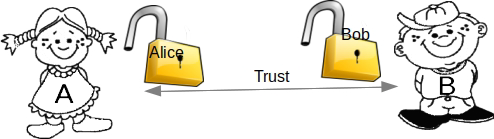
\includegraphics[width=9cm]{images/directtrust.png}
    \caption{Alice vertraut Bob durch direkte Überprüfung}
    \label{directtrust}
    \end{center}
\end{figure}
\begin{itemize}[noitemsep,topsep=0pt,leftmargin=*]
    \item Persönliche Überprüfung
    \item Vorinstalliert in System oder Software (z.B. Public Key von Google-Server in Chrome, Apps, VPN-Clients)
    \item Publiziert auf Webseite oder in Zeitung
\end{itemize}
Benötigt jedoch einen authentischen Kanal zum Etablieren des Trust.

\paragraph*{Web of Trust (WOT)}
Alice vertraut der Authentizität von Daves Public Key, weil dieser von Charlie signiert wurde, dessen Public Key wiederum von Bob signiert wurde, dem sie vertraut.
\begin{figure}[H]
    \begin{center}
    \includegraphics[width=12cm]{images/wot.png}
    \caption{Alice vertraut Dave indirekt durch Vertrauensnetz}
    \label{wot}
    \end{center}
\end{figure}

\paragraph*{Hierarchial Trust (PKI)}Eine \textsl{Public Key Insfrastructure (PKI)} ist ein System, das digitale Zertifikate ausstellen, verteilen und Prüfen kann. Im Gegensatz zum WOT ist eine PKI hierarchisch aufgebaut und bedingt deshalb Root Certification Authorities, welche über alle anderen Zertifizierungstellen steht.
\begin{figure}[H]
    \begin{center}
    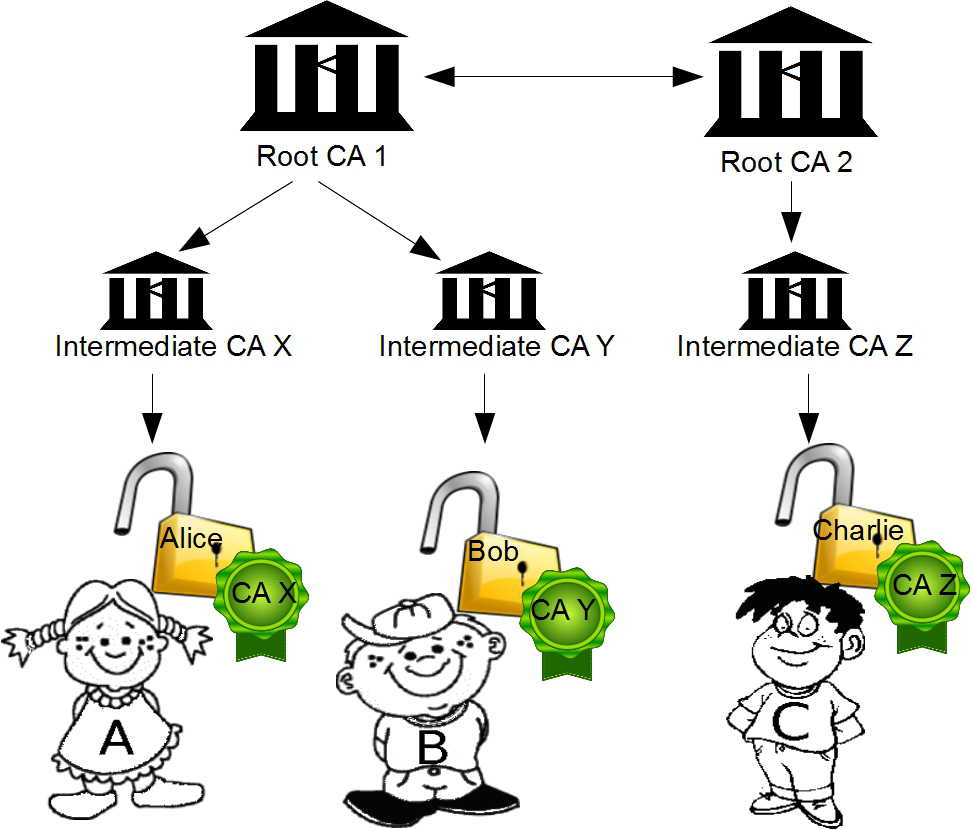
\includegraphics[width=8cm]{images/ht.png}
    \caption{Hierarchical Trust durch Certificate Authorities}
    \label{ht}
    \end{center}
\end{figure}


\subsection*{Sie wissen was eine Public-Key-Infrastruktur, eine Certificate Authority und ein Zertifikat ist, wofür und wie diese verwendet werden und wie Zertifikate ausgestellt und revoziert werden}

\paragraph*{Grundbegriffe PKI}Die Zertifizierungstelle \textsl{Certificate Authority (CA)}\newline
Eine CA ist eine Organisation, welche digital eZertifikate ausstellt. Ein digitales Zertifikat ordnet einen bestimmten öffentlichen Schlüssel einer Person oder Organisation zu. Diese Zuordnung wird von der Zertifizierungstelle beglaubigt, indem sie sie mit ihrer eigenen digitalen Unterschrift versieht.\newline
Ein Zertifikat wird durch eine sog. \textsl{Chain of Trust} beglaubigt. Eine \textsl{intermediate CA} signiert das Zertifikat (Public Key) des Endbenutzers. Das Zertifikat der intermediate CA wird wiederum von einer anderen CA unterschrieben. Das letzte Zertifikat in dieser Kette heisst \textsl{Root Certificate} und enthält den Public Key der \textsl{root CA}. Dieses Zertifikat ist normalerweise \textsl{self signed}, also von der root CA selbst unterschrieben.


\subsection*{Sie wissen was SSL/TLS ist, welche Funktionalität es erreicht und wie das Protokoll konzeptionelle abläuft}SSL-TLS erreicht
\begin{itemize}[noitemsep,topsep=0pt,leftmargin=*]
    \item Authentisierung des Servers gegenüber dem Client
    \item \textsl{Optional}: Authentisierung des Clients gegenüber dem Server (`mutual SSL')
    \item Verschlüsselung und Authentisierung der Daten
\end{itemize}
Das SSL/TLS-Protokoll läuft in \underline{zwei Phasen} ab:
\begin{itemize}[noitemsep,topsep=0pt,leftmargin=*]
    \item \textbf{Handshake}: vereinbart mittels Public-Key-Kryptographie einen Schlüssel
    \item \textbf{Datenaustausch}: verwendet Secret-Key-Kryptographie zum Verschlüsseln und Authentisieren
\end{itemize}
Beispiele für SSL/TLS-ciphers:
\begin{itemize}[noitemsep,topsep=0pt,leftmargin=*]
    \item \verb|TLS_RSA_WITH_3DES_EDE_CBC_SHA|
    \item \verb|TLS_ECDHE_ECDSA_WITH_AES_256_CBC_SHA384|
\end{itemize}

\subsection*{Kontrollfragen SW 04}
\paragraph*{Was prüfen Sie alles bei einer Authentisierung mittels Zertifikat?}\index{Authentisierung}\index{Zertifikat}
\begin{itemize}[noitemsep,topsep=0pt,leftmargin=*]
    \item Ist das Zertifikat gültig? (Nicht abgelaufen, nicht revoziert)
    \item Ist das Zertifikat und die gesamte Zertifikatskette korrekt signiert?
    \item Traue ich der Root-CA der Zertifikatskette?
    \item Besitzt "`Bob"' den zum Zertifikat gehörenden Private Key?
    \begin{itemize}[noitemsep,topsep=0pt,leftmargin=*]
        \item $VERIFY_{public\,key\,Bob}(response)$
    \end{itemize}
\end{itemize}

\paragraph*{Eine CA hat Ihnen ein Intermediate-CA-Zertifikat ausgestellt, anstelle des bestellten Serverzertifikats. Erklären Sie, wie Sie nun vorgehen, um sich als Google auszugeben. Angenommen Sie können einen Man-in-the-Middle-Angriff machen. Können Sie nun Ihre eigene Webseite anstelle der Google-Seite anzeigen?}
\paragraph*{TODO}


%%%%%%%%%%
\part{Angriffe (SW~05-06)}
\section{Angriffe auf Webanwendungen}

\paragraph*{Bedrohungen auf Anwendungsebene}Webanwendung, Session, Headers, CSRF

\subsection*{Sie wissen was eine Webanwendung ausmacht, wie HTTP funktioniert}
Was unterscheidet eine Webanwendung aus Sicherheitssicht zu anderen Anwendungen?
\begin{itemize}[noitemsep,topsep=0pt,leftmargin=*]
    \item Kommuniziert über HTTP mit einem Server
    \begin{itemize}[noitemsep,topsep=0pt,leftmargin=*]
        \item zustandsloses Protokoll
    \end{itemize}
    \item Läuft in einem Browser
    \begin{itemize}[noitemsep,topsep=0pt,leftmargin=*]
        \item Mehrere Webanwendungen können parallel im gleichen Browser laufen
        \item Die Webanwendung \textsl{erbt} vom Browser implementierte Features
        bzw. muss diese richtig ansprechen
    \end{itemize}
\end{itemize}

\paragraph*{HTTP}Der Browser kommuniziert mit dem Webserver über das \textbf{Hypertext Transfer Protokoll (HTTP)}. HTTP besteht aus \textsl{Requests} und \textsl{Reponses}.

\paragraph*{HTTP-Request-Methoden}Die häufigsten HTTP-Request-Methoden sind \textbf{GET} und \textbf{POST}.
Es existieren aber auch \textbf{PUT, HEAD, DELETE, PATCH, OPTIONS}.

\paragraph*{GET}\verb|https://www.hslu.ch/?p=5 HTTP/1.1|\\
\verb|User-Agent: Mozilla/5.0|
\begin{itemize}[noitemsep,topsep=0pt,leftmargin=*]
    \item Message Body: kein
    \item Ruft Daten vom Server ab
    \item Sollte Serverzustand nicht verändern
\end{itemize}

\paragraph*{POST}\verb|https://www.hslu.ch/ HTTP/1.1|\\
\verb|User-Agent: Mozilla/5.0|
\begin{itemize}[noitemsep,topsep=0pt,leftmargin=*]
    \item Message Body: \verb|id=123&pwd=password|
    \item Darf Serverzustand verändern
    \item Wird nicht gecachet
\end{itemize}

\paragraph*{Häufigste Reponse-Codes}
\begin{itemize}[noitemsep,topsep=0pt,leftmargin=*]
    \item 200 OK
    \item 204 No Content
    \item 301 Moved Permanently
    \item 302 Found (Vorher: "`Moved temporarely"')
    \item 304 Not Modified
    \item 400 Bad Request
    \item 403 Forbidden
    \item 404 Not Found
    \item 500 Internal Server Error
\end{itemize}

\paragraph*{HTTP Zustand} HTTP ist ein zustandsloses Protokoll, d.h. es hat kein `Gedächtnis', bzw. Erinnerung.
\begin{figure}[H]
    \begin{center}
    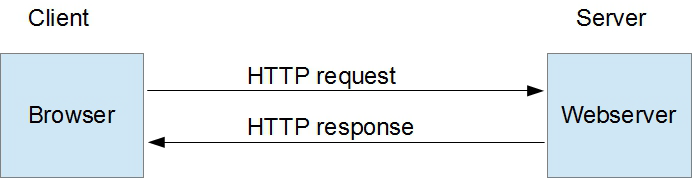
\includegraphics[width=12cm]{images/HTTPZustand0.png}
    \caption{HTTP zustandslos}
    \label{HTTPZustandslos}
    \end{center}
\end{figure}
\noindent
Die einzige Möglichkeit einen Zustand an den Client zu übergeben ist, diesen per weiteren Requests mitzuschicken. Die Zustände werde mit einem Cookie oder einem "`Hidden field"' erfasst.
\begin{figure}[H]
    \begin{center}
    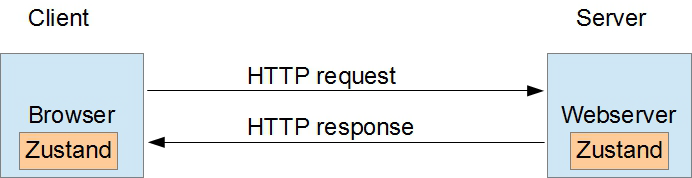
\includegraphics[width=12cm]{images/HTTPZustand1.png}
    \caption{HTTP Zustand per Request (hidden field)}
    \label{HTTPZustand}
    \end{center}
\end{figure}

\paragraph*{Cookies}Cookies sind kurze Textdaten, welche vom Server als Header an den Browser übermittelt werden und von diesem ebenso als Header bei requests wieder mitgesendet werden. Cookies werden vom Browser verwaltet. Die meistgenutzte Möglichkeit ist es, ein Cookie zu setzen. Jedoch dürfen auch Cookies nicht client-seitig angepasst werden können!
\begin{figure}[H]
    \begin{center}
    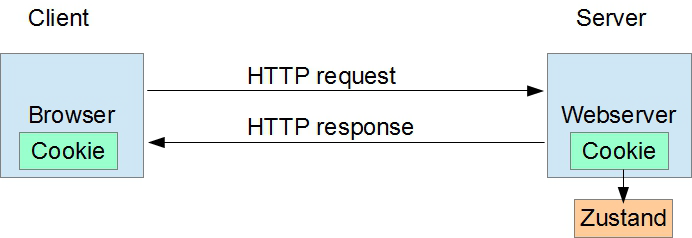
\includegraphics[width=12cm]{images/HTTPCookie.png}
    \caption{Einsatz eines Cookies}
    \label{HTTPCookie}
    \end{center}
\end{figure}

\paragraph*{Cookie Eigenschaften}Die Eigenschaften von Cookies sind:
\begin{itemize}[noitemsep,topsep=0pt,leftmargin=*]
    \item \textbf{Persistent} (mit Ablaufdatum) oder \textbf{Session-Cookie} (ohne Ablaufdatum)
    \item \textbf{Secure} (wird nur über HTTPS übertragen)
    \item \textbf{HTTP Only} (darf nur von HTTP gelesen werden)
    \item \textbf{Same Site} (wird nicht bei Cross-Domain-Aurfrufen mitgesendet, z.B. `embedded' Link, Image)
\end{itemize}


\subsection*{Sie wissen was eine Session ist und welche Eigenschaften einer Session bei welchen Angriffen wichtig sind bzw wie sie gegen gewisse Angriffe Schutz bieten}

\paragraph*{Session} Eine Session ist der Zeitraum, in dem ein Client eine stehende Verbindung mit einem Server hat; vom Login bis zum Logout. Der Server vergibt dem Client eine eindeutige Session-ID. Die Sitzungsdaten (z.B. Warenkorb) werden im Server gespeichert. Bei jedem Request gibt der Client seine Session-ID mit, damit der Server beim Response die zugehörigen Daten dieser ID übermitteln kann. Es gibt auch Sessions ohne stehende Verbindung (ohne Login). Dies wird zu Statistikzwecken verwendet, z.B. um die Bewegung des Besuchers auf der Website zu verfolgen. Oder aber auch um einen Warenkorb ohne Login verwenden zu können.

\paragraph*{Schwaches Session-Management}Was ist das?
\begin{itemize}[noitemsep,topsep=0pt,leftmargin=*]
    \item der Sessionwert ist vorhersagbar
    \item der Sessionwert kann vom Client gesetzt werden
    \item die Cookie-Attribute `Secure', `HttpOnly' oder `Same Site' sind nicht gesetzt
    \item Cookie-Domain oder -Pfad sind nicht so eingeschränkt wie möglich
    \item die Session wird bei einem Logout nicht invalidiert
    \item die Session hat kein server-seitiges Timeout (Inaktivitäts- und absolutes Timeout)
\end{itemize}

\paragraph*{Schwaches Session-Management}Was kann man dagegen tun?
\begin{itemize}[noitemsep,topsep=0pt,leftmargin=*]
    \item lange und kryptographisch zufällige Sessionwerte wählen
    \item nur vom Server gewählte Sessionwerte akzeptieren
    \item Cookies als `Secure',`HttpOnly' oder `Same Site' mit so eingeschränkter Domain und Pfad wie möglich setzten
    \item Session \textbf{server-seitig} bei einem Logout oder Timeout invalidieren
\end{itemize}

\paragraph*{Same Origin Policy}Mehrere Webanwendungen können im gleichen Browser parallel laufen. Die Same-Origin-Policy verhindert, dass eine parallel laufende Webanwendungen uneingeschränkt
\begin{itemize}[noitemsep,topsep=0pt,leftmargin=*]
    \item auf die Daten einer anderen Anwendung zugreifen
    \item die Cookies einer anderen Anwendung lesen oder mitschicken
    \item Requests auf die andere Anwendung absetzen
\end{itemize} kann.\\
Same Origin Policies im Browser gibt es z.B. für Cookies, DOM access (Zugang zu document.cookie), HTML5Storage, XMLHttpRequests.

\paragraph*{Same Origin Policy: Cookies} Cookies haben eine \textbf{domain} und \textbf{path}.
\begin{itemize}[noitemsep,topsep=0pt,leftmargin=*]
    \item \textbf{Setzen des Cookies:} Nur Domain-Suffix des URL-Hostname dürfen gesetzt werden. (Aber keine Top-Level Domains!)\\
    Path kann beliebig gesetzt werden.
    \item \textbf{Senden des Cookies:} Cookies werden nur dann mitgeschickt, wenn die Cookie-Domain ein Domain-Suffix der URL-Domain und der Cookie-Path ein Prefix des URL-Path ist.
\end{itemize}

\paragraph*{Session Fixation}Was ist das?\\
Der Sessionwert wird nach einem Login oder Loginschritt nicht geändert. Ein  angreifer mit Zugang zu einer unauthentisierten Session kann warten bis ein Benutzer sich einloggt und ist damit selbst eingeloggt.

\paragraph*{Session Fixation}Was kann man dagegen tun?\\
Sessionwert nach jedem Authentisierungsschritt ändern.

\subsection*{Sie kennen sicherheitsrelevante Header}

\paragraph*{Sicherheitsrelevante Response-Header}
\begin{enumerate}[noitemsep,topsep=0pt,leftmargin=*]
    \item \textbf{HSTS:} \verb|Strict-Transport-Security: max-age=31536000; includeSubDomains|\\
    Seite wird nur via HTTPS aufgerufen. \verb|max-age| muss hoch gesetzt werden!
    \item \textbf{Frame-Options:} \verb|X-Frame-Options: deny|\\
    Verbietet das Einbinden der Seite in einem Frame oder erlaub es nur für bestimmte Domains
    \item \textbf{XSS-Protection:} \verb|X-XSS-Protection: 1; mode=block|\\
    Filtert und säubert oder blockeirt die Anzeige der Seide, wenn ein XSS-Angriff endeckt wird
    \item \textbf{Content-Type-Options:} \verb|X-Content-Type-Options: nosniff|\\
    Verhindert, dass der Content als einen anderen MIME-Type interpretiert wird als angegeben
    \item \textbf{CSP:} \verb|Content-Security-Policy: script-src \textquotesingle self\textquotesingle|\\
    Definiert, welche Resourcen (z.B. Bilder, Scripts, Fonts, etc.) von wo eingebunden werden können
    \item \textbf{CORS} \verb|Access-Control-Allow-Origin: http://foo.example|\\
    Cross-Origin Resource Sharing (CORS) ist ein Mechanismus, der Webbrowsern oder auch anderen Webclients Cross-Origin-Requests ermöglicht. Zugriffe dieser Art sind normalerweise durch die Same-Origin-Policy (SOP) untersagt. CORS ist ein Kompromiss zugunsten grösserer Flexibilität im Internet unter Berücksichtigung möglichst hoher Sicherheitsmassnahmen.
    \item \textbf{Caching-Options} {\color{red}TODO: hat jemand Infos?}
    \item \textbf{HPKP ({\color{red}deprecated!}):}
    \verb|Public-Key-Pins:|\\
    \verb|pin-sha256="d6qzRu9zOECb90Uez27xWltNsj0e1Md7GkYYkVoZWmM=";|\\
    \verb|pin-sha256="Ë9CZ9INDbd+2eRQozYqqbQ2yXLVKB9+xcprMF+44U1g=";|\\
    \verb|report-uri=http://example.com/pkp-report;|\\
    \verb|max-age=10000; includeSubDomains|\\
    HTTP Public Key Pinning: Nur das Serverzertifikat mit dem korrekten Fingerprint wird akzeptiert. Wurde wieder abgekündigt und die meisten Browser unterstützen es nicht mehr.
\end{enumerate}

\subsection*{Sie verstehen wie ein Cross-Site-Request-Forgery-Angriff abläuft und wie man sich dagegen schützen kann}

\paragraph*{CSRF - Cross-Site Request Forgery}Was ist das?\\
Der Angreifer bringt einen Benutzer dazu, einen Request aus seinem Browser abzusetzen und  dadurch eine Aktion auf dem Server auszulösen. Ist der Benutzer zu dem Zeitpunkt eingeloggt, wird das Cookie automatisch mitgeschickt.
\begin{figure}[H]
    \begin{center}
    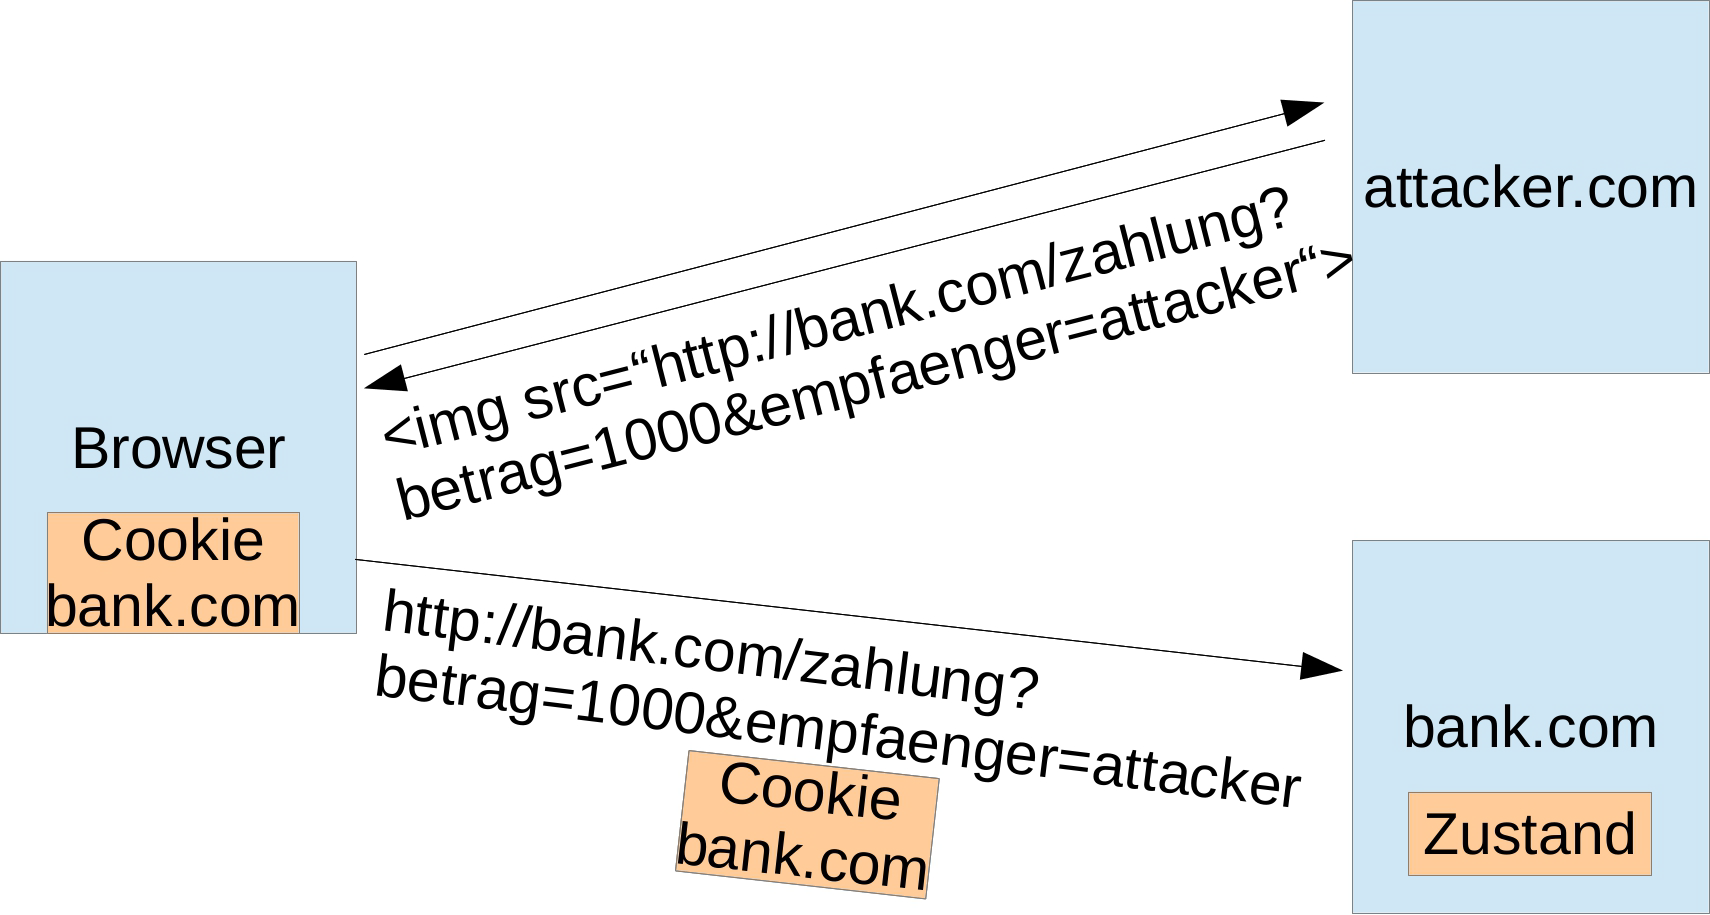
\includegraphics[width=10cm]{images/CSRF.png}
    \caption{Cross-Site Request Forgery}
    \label{CSRF}
    \end{center}
\end{figure}
\paragraph*{CSRF - Cross-Site Request Forgery}Was kann man dagegen tun?
\begin{itemize}[noitemsep,topsep=0pt,leftmargin=*]
    \item \textbf{CSRF-Token:} ein Secret als Teil des Form Field oder Header mitgeben (Secret darf nicht vorhersagbar sein)
    \item \textbf{Zusätzlich:} Same-Site-Attribut setzten
\end{itemize}


\section{Angriffe auf Protokollebene}
\subsection*{Sie kennen die Grundbegriffe der Anwendungssicherheit}
\paragraph*{Bedrohungen auf Protokollebene}Begriffe: Social Engineering, Angriffe auf ARP, TCP/IP, DNS, SSL, HTTP

\subsection*{Kurzübersicht}
\index{Bedrohungen auf OSI-Layern}
\begin{itemize}[noitemsep,topsep=0pt,leftmargin=*]
    \item \textbf{Bedrohungen auf Link-Layer:} Spoofing\index{Link-Layer}\index{Spoofing}
    \item \textbf{Bedrohungen auf Transport-Layer:} Denial of Service (DoS)\index{Transport-Layer}\index{DoS}
    \item \textbf{Bedrohungen auf SSL / TLS:} Preisgabe Sensitiver Daten\index{SSL/TLS}\index{Sensitive Daten}
    \item \textbf{Bedrohungen auf Anwendungslayer:} Cross Site Scripting (XSS), Code Injection\index{Anwendungslayer}\index{Cross Site Scripting (XSS)}\index{Code-Injection}\index{XSS! siehe {Cross Site Scripting (XSS)}}
    \item \textbf{Bedrohungen auf Layer 8 (Mensch):} Social Engineering\index{Layer 8}\index{Social Engineering}
\end{itemize}

\index{Fehler vs. Bugs}
\paragraph*{Flaws vs. Bugs} Bei Softwaredefekten wird unterschieden zwischen Flaws und Bugs
\begin{itemize}[noitemsep,topsep=0pt,leftmargin=*]
    \item \textbf{Flaw:} Ein Flaw ist ein Defekt im Design der Software\index{Flaw}
    \item \textbf{Bug:} Ein Bug ist ein Defekt in der Implementation\index{Bug}
\end{itemize}

\paragraph*{Grundbegriffe: Bedrohung}
\index{Threat vs. Threat Agent}\index{Threat}
\begin{itemize}[noitemsep,topsep=0pt,leftmargin=*]
    \item \textbf{Threat:} Möglicher Grund für einen ungewollten Vorfall, der das System oder die Organisation schädigen kann.
    \item \textbf{Threat Agent:} Individuum oder Gruppe welche eine Bedrohung darstellt.
\end{itemize}

\index{Aktive vs. Passive Angriffe}
\subsubsection*{Aktive vs. passive Angriffe}
Bei einem \textbf{passiven Angriff} hält sich der Angreifer an das protokoll. Er verändert z.B. die ausgetauschten Nachrichten nicht hört aber die Kommunikation ab.
Bei einem \textbf{aktiven Angriff} hält sich der Angreifer nicht an das Protokoll. Er verändert z.B. Nachrichten.

\subsection*{Sie kennen Beispiele von Angriffen auf verschiedenen Ebenen des Protokollstacks und wissen was diese bewirken}

\index{OSI-Modell}
\subsubsection*{OSI-Layers}
Die 7 Tierschichten des OSI-Models, wobei die 8te sich auf den Mensch bezieht.

\begin{figure}[H]
    \begin{center}
    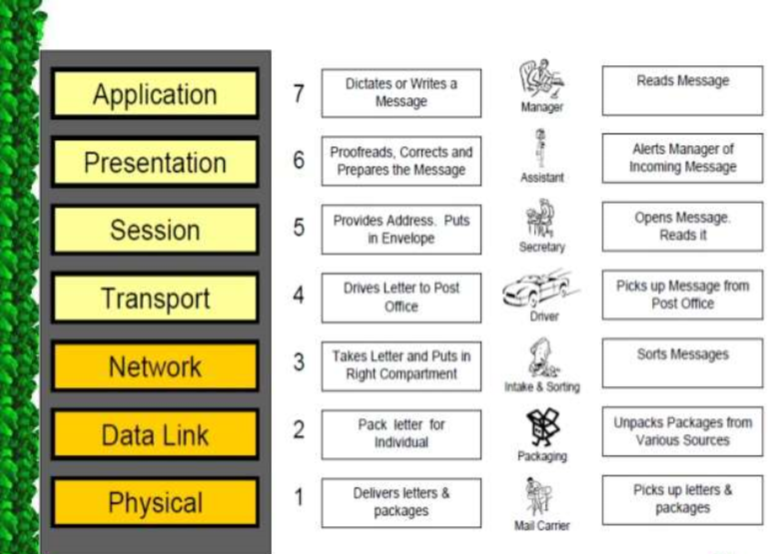
\includegraphics[width=8cm]{images/OSI-Layers.png}
    \caption{OSI-Layers}
    \label{OSI-Layers}
    \end{center}
\end{figure}

\subsubsection*{OSI vs Internet Reference Model}
Die 7 Tierschicht des OSI-Models, wobei die 8te sich auf den Mensch bezieht.

\begin{figure}[H]
    \begin{center}
    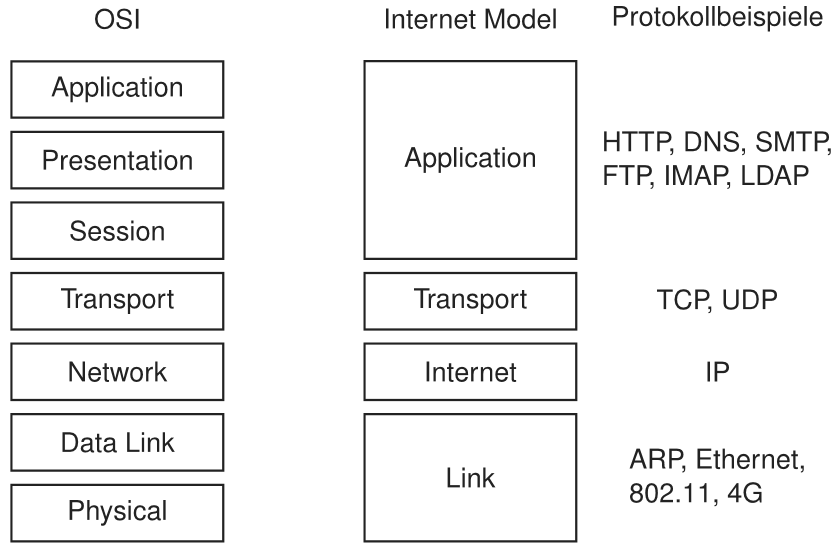
\includegraphics[width=8cm]{images/OSIvsIRM.png}
    \caption{OSI vs. Internet Reference Model}
    \label{OSIvsIRM}
    \end{center}
\end{figure}


\subsubsection*{Encapsulation (Datenkapselung)}
\begin{figure}[H]
    \begin{center}
    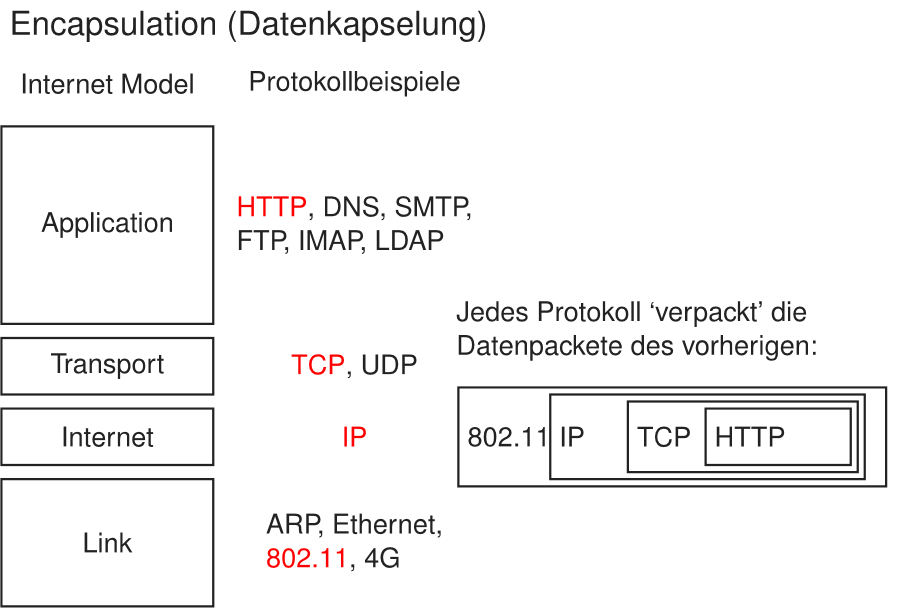
\includegraphics[width=8cm]{images/TCP-Encapsulation.png}
    \caption{TCP-Encapsulation}
    \label{TCP-Encapsulation}
    \end{center}
\end{figure}

\index{ARP-Spoofing}
\subsubsection*{Beispiel: ARP-Spoofing auf dem Link-Layer}
\begin{figure}[H]
    \begin{center}
    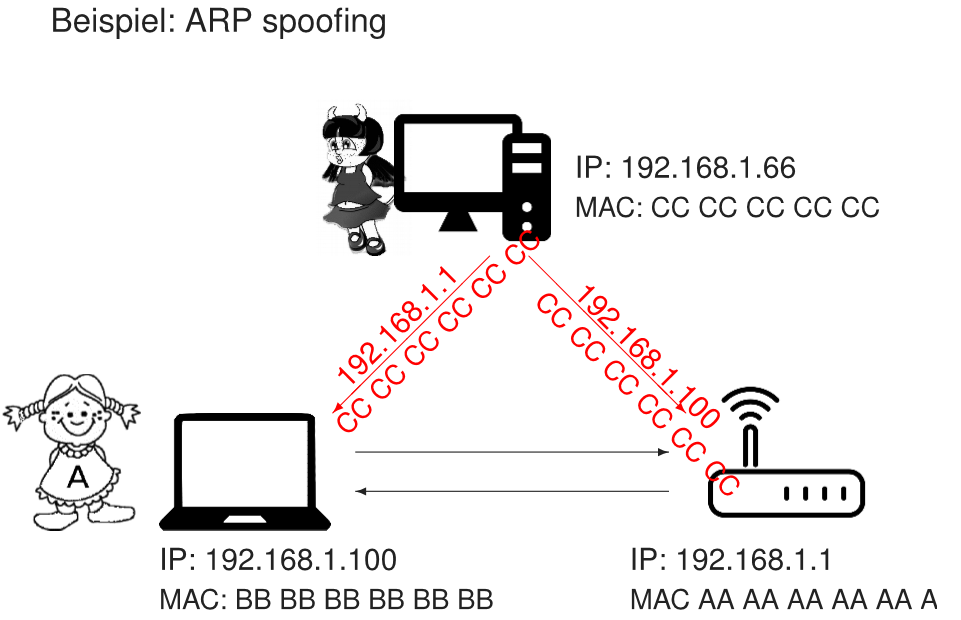
\includegraphics[width=8cm]{images/Beispiel_ARP_Spoofing.png}
    \caption{ARP Spoofing}
    \label{ARP Spoofing}
    \end{center}
\end{figure}

\paragraph*{Spoofing: Was ist das?}
Eine person oder ein Programm gibt sich als jemand anderen oder etwas anderes aus.\\
\textbf{Beispiele:}
\begin{itemize}[noitemsep,topsep=0pt,leftmargin=*]
    \item \textbf{Telefonnummern-Spoofing (Call Centers etc.)}
    \item \textbf{Email-Adressen-Spoofing}
    \item \textbf{IP Spoofing}
    \item \textbf{DNS Spoofing}
    \item \textbf{ARP Spoofing}
    \item \textbf{Content Spoofing}
\end{itemize}
\vspace{0.5cm}
\noindent
"`\textsl{ARP-Spoofing (vom engl. to spoof – dt. täuschen, reinlegen) oder auch ARP Request Poisoning (zu dt. etwa Anfrageverfälschung) bezeichnet das Senden von gefälschten ARP-Paketen. Es wird benutzt, um die ARP-Tabellen in einem Netzwerk so zu verändern, dass anschliessend der Datenverkehr zwischen zwei (oder mehr) Systemen in einem Computernetz abgehört oder manipuliert werden kann. Es ist eine Möglichkeit, einen Man-in-the-Middle-Angriff im lokalen Netz durchzuführen.}"'\cite{wiki}

\paragraph*{Spoofing: Was kann man dagegen tun?}
\paragraph*{Je nach Situation unterschiedlich, zB.:}
\begin{itemize}[noitemsep,topsep=0pt,leftmargin=*]
    \item {Authentisieren}
    \item {Angaben überprüfen}
\end{itemize}

%
\index{3-Way Handshake} \index{TCP Verbindungsaufbau}
\subsubsection*{Repetition: TCP Verbindungsaufbau (vereinfacht)}
\begin{figure}[H]
    \begin{center}
    \includegraphics[width=8cm]{images/Repetition_3_way_handshake.png}
    \caption{3-Way Handshake}
    \label{3-Way Handshake}
    \end{center}
\end{figure}

\index{DoS}
\paragraph*{Bedrohungen auf Transport-Layer:} Denial of Service (DoS)
\paragraph*{Denial of Service}Syn-Nachrichten werden mit gespoofter IP gesendet. Syn-Acknowledgements Nachrichten gehen nirgendwo hin.
Server wird überflutet mit Abfragen und kann nicht schneller abarbeiten als Sie reinkommen.
Als Resultat kann somit von den meisten Benutzern die Seite nicht angezeigt werden.
\begin{figure}[H]
    \begin{center}
    \includegraphics[width=8cm]{images/Syn-flood.png}
    \caption{SYN Flood}
    \label{Syn Flood}
    \end{center}
\end{figure}

\index{DRDoS}
\paragraph*{Beispiel: Distributed Reflection Denial of Service}
\noindent
"`\textsl{Hierbei adressiert der Angreifer seine Datenpakete nicht direkt an das Opfer, sondern an regulär arbeitende Internetdienste, trägt jedoch als Absenderadresse die des Opfers ein (IP-Spoofing). Die Antworten auf diese Anfragen stellen dann für das Opfer den eigentlichen DoS-Angriff dar. Durch diese Vorgehensweise ist der Ursprung des Angriffs für den Angegriffenen nicht mehr direkt ermittelbar.}"' - Wikipedia

\begin{figure}[H]
    \begin{center}
    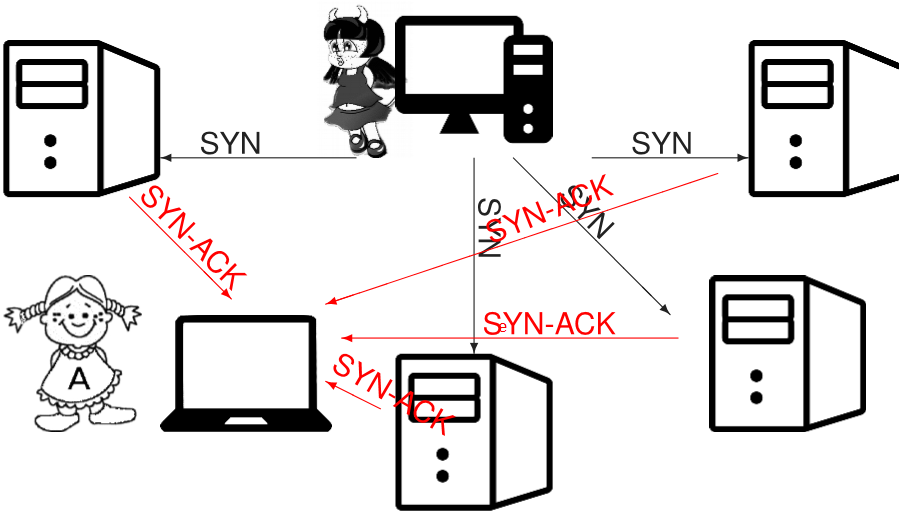
\includegraphics[width=8cm]{images/DRDoS.png}
    \caption{DRDoS}
    \label{DRDoS}
    \end{center}
\end{figure}

\paragraph*{Denial of Service: Was kann man dagegen tun?} Jedes System bricht irgendwann zusammen! Es geht darum sicherzustellen, dass dabei keine bleibenden Schäden am
Kernsystem entstehen und das System nach einem Angriff schnell wieder funktionsfähig zu machen.

\subsubsection*{Schutzbeispiele:}
\begin{itemize}[noitemsep,topsep=0pt,leftmargin=*]
    \item \textbf{Beschränkung der Anzahl (Web-) Requests pro Zeiteinheit / IP }
    \item \textbf{Sicherstellen, dass der "`Flaschenhals"' weit vorne auftritt (z.B. Firewall) um Kernsysteme zu schützen}
    \item \textbf{Sicherstellen, dass das System sich nicht selbst überlastet durch freigeben nicht mehr verwendeter Ressourcen, vermeiden von undendlichen Loops etc.}
    \item \textbf{Disaster Recovery Plan}
\end{itemize}

\subsubsection*{SSL/TLS im internet Modell}\index{SSL/TLS}
\begin{figure}[H]
    \begin{center}
    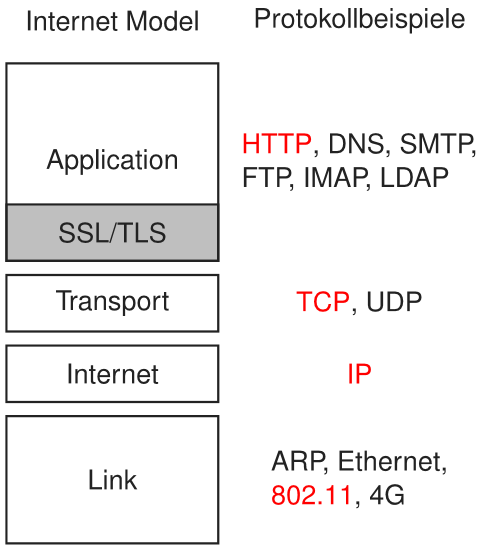
\includegraphics[width=8cm]{images/SSL-TLS.png}
    \caption{SSL/TLS}
    \label{SSL/TLS}
    \end{center}
\end{figure}

\subsubsection*{Bedrohung auf SSL / TLS (Preigabe Sensitiver Daten)}

\index{Sensitive Daten}
\paragraph*{Preisgaber Sensitiver Daten: Was ist das?} Angreifer stehlen Schlüssel, Passwörter, Geschäftsgeheimnsisse,
Personendaten oder andere sensitive Daten vom Server, bei der Übertragung oder vom Client

\paragraph*{Preisgabe sensitiver Daten: Was kann man dagegen tun?}
\begin{itemize}[noitemsep,topsep=0pt,leftmargin=*]
    \item Keine Daten speichern oder übertragen, welche nicht benötigt werden.
    \item Daten nach ihrer Sensivität klassifizieren und entsprechend behandeln
    \item Sensitive Daten nur gespeichert auf dem Server ablegen
    \item Passwörter mit Salt und Pepper und einer starken Passwort-Hashfunktion gehasht ablegen.
    \item Daten verschlüsselt übertragen (FTP$\Rightarrow$SFTP, HTTP$\Rightarrow$HTTPS, etc). Zertifikat überprüfen!
    \item Sicherstellen, dass sichere Ciphers verwendet werden
    \item Keine sensitiven Daten auf der Clientseite cachen.
\end{itemize}

\subsubsection*{Bedrohungen auf Anwendungslayer: Cross Site Scripting (XSS) und Code Injection}
\index{Cross Site Scripting (XSS)}\index{XSS! siehe {Cross Site Scripting (XSS)}}
\paragraph*{XSS: Was ist das?}Ein Angreifer bringt den legitimen Server dazu ein Script an den Browser zu senden. Dieses wird im Kontext des legitimen Servers ausgeführt. Es wird zwischen \textbf{stored} und \textbf{reflected} XSS unterschieden
\begin{figure}[H]
    \begin{center}
    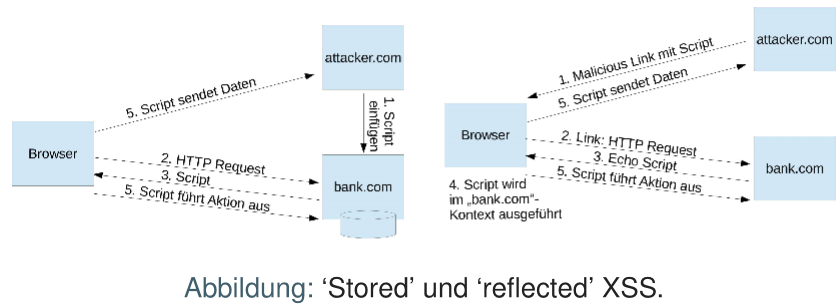
\includegraphics[width=15cm]{images/XSS.png}
    \caption{XSS}
    \label{XSS}
    \end{center}
\end{figure}

\paragraph*{XSS: was kann man dagegen tun?}
\begin{itemize}[noitemsep,topsep=0pt,leftmargin=*]
    \item \textbf {Escaping} aller unsicheren Daten (z.B. vom Benutzer eingegebene) bevor sie angezeigt werden.\\ Bsp. Ersetzen von \textbf{\& \textless \textgreater \textquotedblleft \textquoteright} durch \textbf{\&amp; \&lt; \&gt; \&quot; \&\#x27; \&\#x2F;}
\end{itemize}
\paragraph*{}Zusätzlich sollen folgende Massnahmen getroffen werden:
\begin{itemize}[noitemsep,topsep=0pt,leftmargin=*]
    \item Cookie als \texttt{HttpOnly}-Cookie setzen
    \item Header-Felder setzen\\ Bsp. Content-Security-Policy: \verb|default-src: 'self'; script-src: 'self' static.domain.tld| \\ Bsp. \verb|X-XSS-Protection: 1; mode=block|
\end{itemize}

\index{Code Injection}
\paragraph*{Code Injection: Was ist das?} Vermischung von `Code' und `Daten'
\begin{figure}[H]
    \begin{center}
    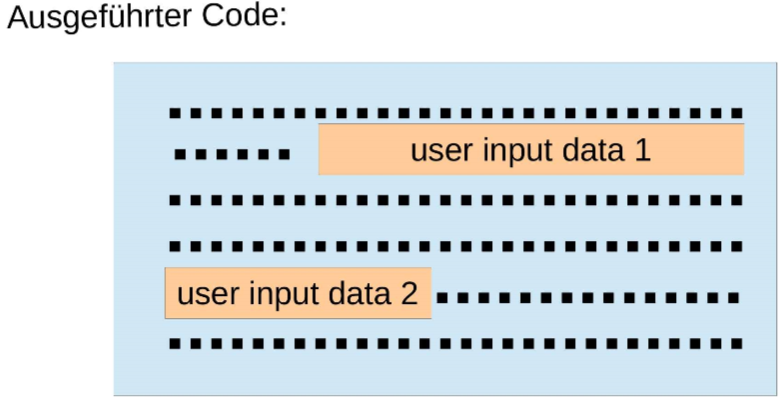
\includegraphics[width=8cm]{images/Code-Injection.png}
    \caption{Code Injection}
    \label{Code Injection}
    \end{center}
\end{figure}

\begin{figure}[H]
    \begin{center}
    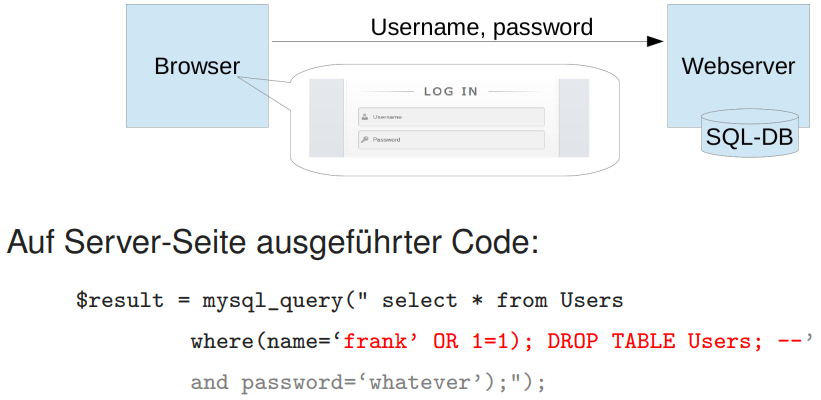
\includegraphics[width=12cm]{images/Bsp-Code-Injection.png}
    \caption{Beispiel Code Injection}
    \label{Code Injection example}
    \end{center}
\end{figure}

\paragraph*{Code Injection: Was kann man dagegen tun?}
\begin{itemize}[noitemsep,topsep=0pt,leftmargin=*]
    \item `Prepared statements' verwenden \\ Beispiel:\\
    \verb|$statement = $db->prepare('SELECT * FROM Users WHERE(name=? password=?);';|\\
    \verb|$stmt->bind_param('ss', $user, $pass);|
    \item Whitelisting der Inputs
    \item Sanitizing der Inputs \\ Bsp. Löschen von Zeichen wie \verb|';-| oder Ersetzen durch `sichere' Zeichen wie \verb|\'\;\-|
    \item Rechte des technischen Benutzers auf der DB einschränken
    \item Verwenden eines sicheren APIs
\end{itemize}

\index{Layer 8}\index{Layer 8}
\subsubsection*{Layer 8}
\begin{figure}[H]
    \begin{center}
    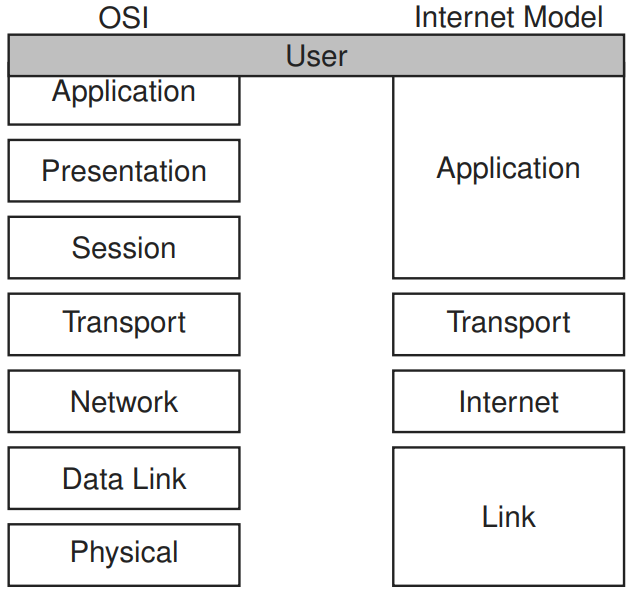
\includegraphics[width=8cm]{images/Layer8.png}
    \caption{Layer 8, der User}
    \label{Layer 8}
    \end{center}
\end{figure}

\index{Social Engineering}
\paragraph*{Social Engineering: Was ist das?}Zwischenmenschliche Beeinflussungen mit dem Ziel, bei
Personen bestimmte Verhaltensweisen hervorzurufen, sie zum
Beispiel zur Preisgabe von vertraulichen Informationen, zum
Kauf eines Produktes oder zur Freigabe von Finanzmitteln zu
bewegen.

\paragraph*{Social Engineering: Was kann man dagegen tun?}
\begin{itemize}[noitemsep,topsep=0pt,leftmargin=*]
    \item Benutzer schulen ('awareness')
    \item Für den Benutzer verständliche Abläufe Sicherstellen
    \item Benutzer nicht zum Umgehen von Sicherheitsmassnahmen verleiten
    \item Fraud Detection-Massnahmen
    \item Technische Massnahmen welche den Angriff verhindern, z.B. Vereinzelungsanlage, nicht vorlesbare Codes etc.
\end{itemize}



\paragraph*{TODO}


%%%%%%%%%%
\part{Management (SW~07-09)}
\section{Standards \& Frameworks, ISMS}

\subsection*{Sie wissen, was ein ISMS ist und wie man damit umgeht}
\paragraph*{ISMS}\index{ISMS}Ein \textsl{Information Security Management System (ISMS)} (auf Deutsch: Managementsystem für die Informationssicherheit) definiert Regeln, Methoden und Abläufe, um die IT-Sicherheit in einem Unternehmen zu gewährleisten, zu steuern, zu kontrollieren und zu optimieren.
\paragraph*{Zweck}
\begin{itemize}[noitemsep,topsep=0pt,leftmargin=*]
    \item Die (durch die IT verursachte) Risiken sollen identifizierbar und beherrschbar werden.
    \item Sicherheit erhalten, dass teure Informationen und Daten der Unternehmung angemessen geschützt sind.
    \item Rechtliche (Datenschutz- oder Berufsgesetz bei Ärzten / Anwälte) und auch Marktanforderung erfüllen (wenn morgen in den Medien publik wird, dass bei der UBS Bank «gehakt» und Millionen gestohlen wurde, dann würden die Kunden nicht länger ihr Vermögen bei der UBS deponieren.
\end{itemize}
\paragraph*{Vorgehen}
\begin{itemize}[noitemsep,topsep=0pt,leftmargin=*]
    \item Man sollte einen Prozess unterhalten, mit dem die Risiken der Informationssicherheit identifiziert und bewertet werden können. Dazu sollen Kontrollen bestimmt, eingeführt und stetig verbessert werden können.
    \item Davor muss zuerst der Schutzbedarf von Vermögenswerten bestimmt und Schutzmassnahmen eingeführt werden.
\end{itemize}

\subsection*{Sie kennen die wichtigsten Standards der Informationssicherheit}
\paragraph*{Standards}\index{ISO Standards}
\begin{itemize}[noitemsep,topsep=0pt,leftmargin=*]
    \item ISO 27000: ISMS – Overview and vocabulary (Überblick / Index)
    \item ISO 27001: ISMS – Requirements (Anforderungskatalog)
    \item ISO 27002: Code of practice for information security controls (Analog: Kochbuch; darin steht drin, welche Massnahmen ich tätigen muss)
    \item ISO 27003: implementation guidance (wie ich die Anforderung umsetze)
    \item ISO 27004: Information security management – Measurement (Ziele müssen messbar sein, z.B. Jahresziele beim Mitarbeiter Gespräch; Ende Periode kann überprüft werden, ob die Ziele erreicht wurden
    \item ISO 27005: Information security risk management (Risiko Bewältigung)
\end{itemize}

\begin{figure}[H]
\paragraph*{Überblick der Zusammenhänge}
    \begin{center}
    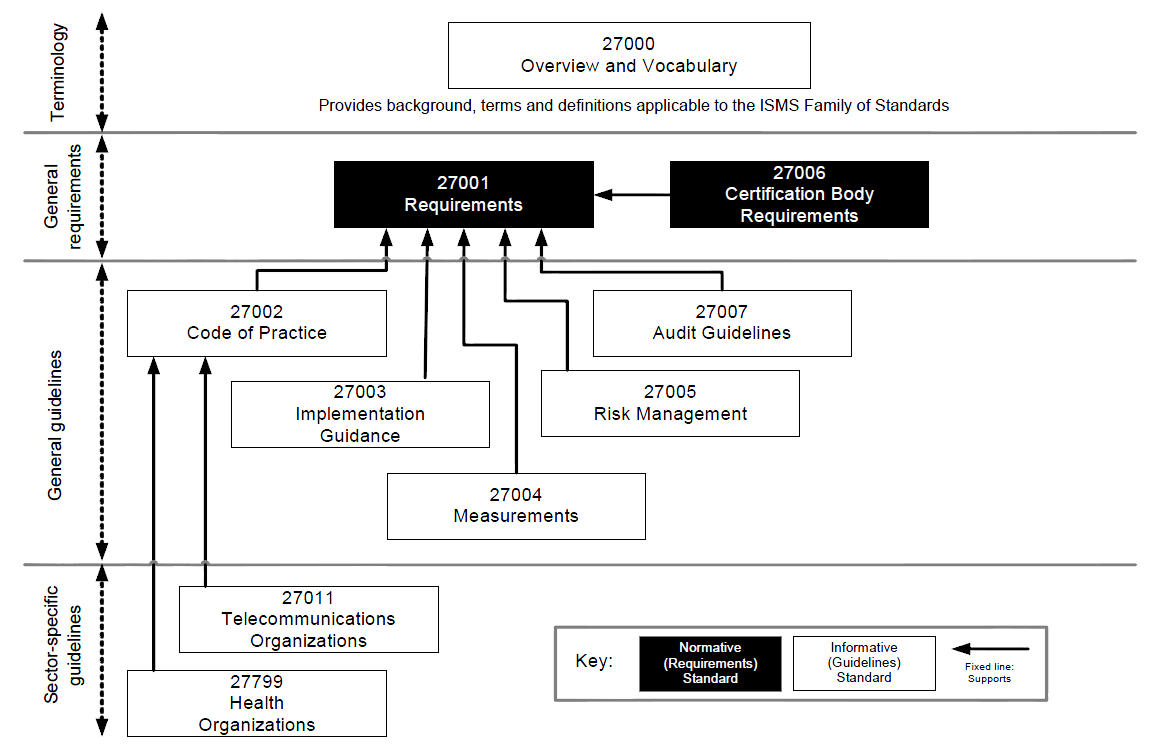
\includegraphics[width=16cm]{images/iso27000.png}
    \caption{Zusamenhang der verschiedenen ISO Standards \cite{iso27000}}
    \label{iso27000}
    \end{center}
\end{figure}

\paragraph*{ISO 27000 - Overview and vocabulary}\index{ISO Standards!ISO 27000}\label{para:ISO 27000}
\begin{itemize}[noitemsep,topsep=0pt,leftmargin=*]
    \item Definiert Begriffe, welche in der ISO 27000 Standard-Reihe verwendet werden
    \item Definiert und erläuternt kurz, was ein Information Security Management System (ISMS) ist
    \item \textsl{Erklärt} den dazu verwendeten Prozess-Ansatz "`Plan - Do - Check - Act"' (PDCA)\index{PDCA!Plan-Do-Check-Act}
    \item Gibt einen Überblick über die ISO 27000 Standard-Reihe
\end{itemize}

\paragraph*{ISO 27001 - Requirements}\index{ISO Standards!ISO 27001}\label{para:ISO 27001}
\begin{itemize}[noitemsep,topsep=0pt,leftmargin=*]
    \item Definiert
    \begin{itemize}[noitemsep,topsep=0pt,leftmargin=*]
        \item Einführung
        \item Betrieb
        \item Überwachung
        \item Wartung
        \item Verbesserung
    \end{itemize}
    eines dokumentierten ISMS's
    \item Wurde aus dem britischen Standard BS 7799-2:2002 entwickelt und als ISO-Norm im Jahr 2005 veröffentlicht
    \item \textsl{Definiert} den Sicherheitsprozess nach dem Prozess-Ansatz PDCA
    \begin{itemize}[noitemsep,topsep=0pt,leftmargin=*]
        \item Dieses Vorgehensmodell wird in ISO 27001:2013 nicht mehr explizit erwähnt, da es auch andere Ansätze gibt, um einen Sicherheitsprozess zu modellieren
    \end{itemize}
    \item Definiert in Anhang A Ziele und Massnahmen zur Verbesserung der Informationssicherheit (die Ziele und Massnahmen sind aus ISO 27002 entlehnt)
    \item Eine Firma kann sich nach ISO 27001 zertifizieren lassen
    \item Freiheitsgrade beim Aufbau eines ISMS
    \begin{itemize}[noitemsep,topsep=0pt,leftmargin=*]
        \item "`Scope"': Bereich, über den sich das ISMS erstreckt
        \begin{itemize}[noitemsep,topsep=0pt,leftmargin=*]
            \item Ganze Firma
            \item Eine Abteilung
            \item Ein Standort
            \item Ein Teil der Infrastruktur: z.B. die DMZ
            \item etc.
        \end{itemize}
        \item Kontrollziele und Steuerungen (\flqq Controls\frqq{} aus ISO 27002), welche vom ISMS berücksichtigt werden ("`Statement of Applicability"', SOA\index{SOA!Statement of Applicability})
    \end{itemize}
    \item "`Scope"' und "`SOA"' definieren dem Umfang einer Zertifizierung nach ISO 27001
\end{itemize}
\begin{figure}[H]
    \begin{center}
    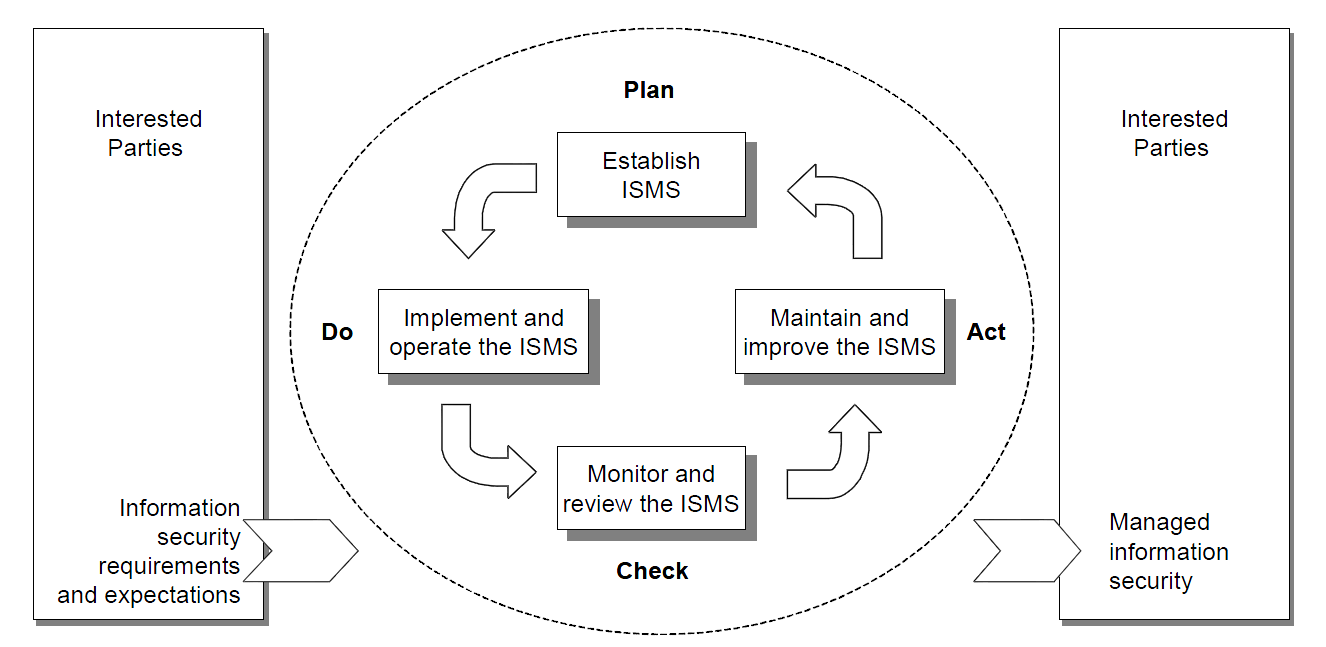
\includegraphics[width=16cm]{images/iso27001.png}
    \caption{Prozess nach ISO 27001 \cite{iso27001}}
    \label{iso27001}
    \end{center}
\end{figure}

\paragraph*{Plan-Do-Check-Act nach ISO 27001}\index{PDCA!Plan-Do-Check-Act}
\begin{itemize}[noitemsep,topsep=0pt,leftmargin=*]
    \item \textbf{Planen (Erstellung des ISMS)}\\
    Erstellung der jeweils für das Risikomanagement und zur Informationssicherheitsverbesserung relevanten ISMS-Richtlinien, Zielsetzungen, Prozesse und Prozeduren zur Erzielung von Ergebnissen gemäss den Gesamtrichtlinien und -zielsetzungen einer Organisation.
    \item \textbf{Machen (Einführung und Durchführung des ISMS)}\\
    Einführung und Durchführung der ISMS-Richtlinien, -Steuerungsmassnahmen, -Prozessen, und -Prozeduren
    \item \textbf{Prüfen (Überprüfung und Revision des ISMS)}\\
    Beurteilung und, wo massgebend, Messung des Prozesserfolgs gegenüber den ISMS-Richtlinien, -Zielsetzungen und praktischen Erfahrungen, sowie Berichterstattung über die Ergebnisse an das Management zwecks Revision
    \item \textbf{Handeln (Wartung und Verbesserung des ISMS)}\\
    Ergreifung korrigiernder und vorbeugender Massnahmen, basierend auf den Ergebnissen des ISMS-Audits und der Management-Revision oder anderen relevandten Informationen zur Erzielung einer laufenden Verbesserung des ISMS
\end{itemize}

\paragraph*{ISO 27002 - Code of practice for information security management}\index{ISO Standards!ISO 27002}\label{para:ISO 27002}
\begin{itemize}[noitemsep,topsep=0pt,leftmargin=*]
    \item Standardwerk zum Thema Informationssicherheit, kurz oft CoP genannt
    \item Definiert 114 Steuerungsmassnahmen\footnote{auch Massnahmen oder Prüfpunkte genannt} für den sicheren Umgang mit Informationen
    \item Zu jeder Massnahme sind Umsetzungsanleitungen angegeben, allerdings jeweils mit nur wenig Detailgrad
    \item Eine Zertifizierung nach ISO 27002 ist nicht möglich, da es keine harten Forderungen gibt (nur \textsl{sollte}-Formulierungen)
    \item Der Standard eignet sich sehr gut zur Umsetzung eines sog. Grundschutzes\index{Grundschutz} (Mindestanforderung im Sicherheitsbereich)
    \item Ursprung aus British Standard BS 7799-1:1999, wurde zu ISO 17799:2000; dann zu ISO 27002:2007 umbenannt, welches wortgleich mit ISO 17799:2005 war.
    \item Aktuell ISO 27002:2013
    \item Adressierte Themen
    \begin{itemize}[noitemsep,topsep=0pt,leftmargin=*]
        \item Organisatorische, physische und logische Sicherheit
        \item Anwendungsentwicklung und -unterhalt
        \item Notfallvorsorge
        \item Einhaltung und Überprüfung der Sicherheit
        \item etc.
    \end{itemize}
\end{itemize}

\begin{figure}[H]
\paragraph*{14 Domänen (Kapitel) von ISO 27002}\index{Domänen}
    \begin{center}
    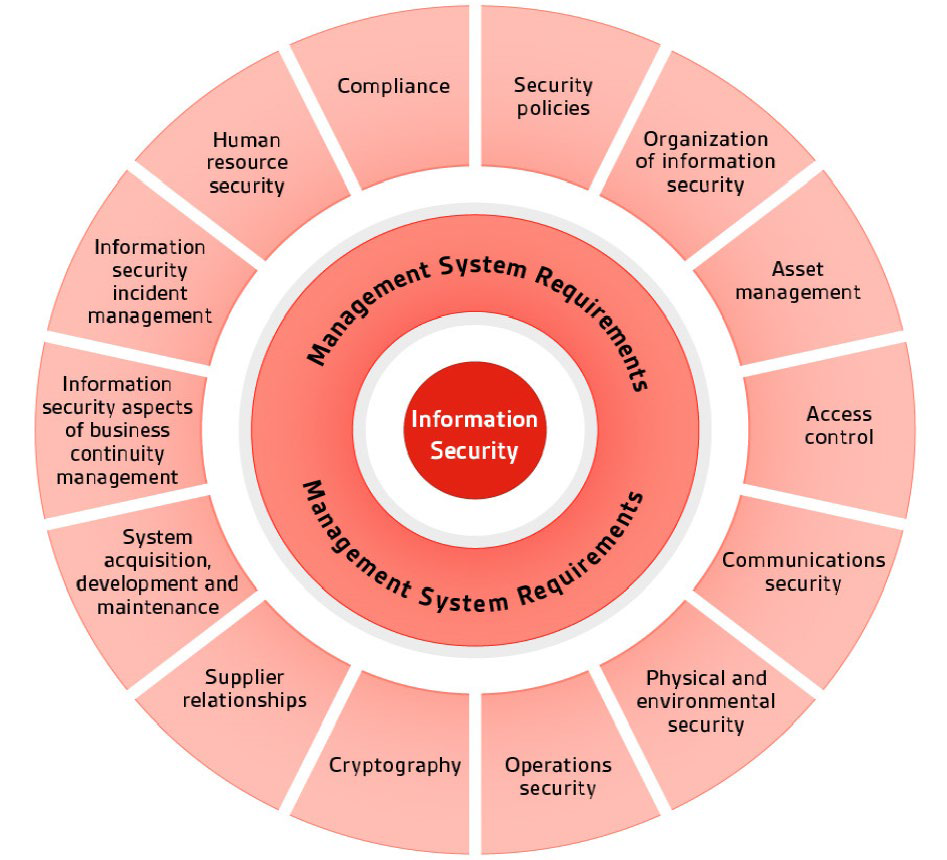
\includegraphics[width=12cm]{images/domains.png}
    \caption{14 Domänen (Kapitel)}
    \label{domains}
    \end{center}
\end{figure}

\paragraph*{ISO 27003 - ISMS implementation guidance}\index{ISO Standards!ISO 27003}\label{para:ISO 27003}
\begin{itemize}[noitemsep,topsep=0pt,leftmargin=*]
    \item Anleitung für die Entwicklung eines Implementierungsplans für eine ISMS nach ISO 27001
    \item Der Standard enthält nur Empfehlungen, jedoch keine Anforderungen
    \item Aufwand für den Aufbau eines ISMS in einer Firma mittlerer Grösse (ca. 250 Mitarbeitende)
    \begin{itemize}[noitemsep,topsep=0pt,leftmargin=*]
        \item 12-18 Monate
        \item Mehrere hunderttausend Franken
    \end{itemize}
\end{itemize}

\paragraph*{ISO 27004 - Information security management - Measurement}\index{ISO Standards!ISO 27004}\label{para:ISO 27004}
\begin{itemize}[noitemsep,topsep=0pt,leftmargin=*]
    \item Anleitung für die implementation eines Messsystems für die Beurteilung der Effektivität eines ISMS und der damit verbundenen Steuerungsmassnahmen gemäss ISO 27002
    \item Der Standard enthält Empfehlungen zu folgenden Aktivitäten:
    \begin{itemize}[noitemsep,topsep=0pt,leftmargin=*]
        \item Entwicklung von Messkritieren
        \item Implementation eines Information Security Measurement Program (ISMP\index{ISMP})
        \item Analyse von Messresultaten und Reporting an die Stakeholders
        \item Nutzung der Resultate, um das ISMS und die zugehörigen Massnahmen, sowie Kontrollen zu verbessern
        \item Nutzung der Resultate, um das ISMP zu verbessern
    \end{itemize}
\end{itemize}

\paragraph*{ISO 27005 - Information security risk management}\index{ISO Standards!ISO 27005}\label{para:ISO 27005}
\begin{itemize}[noitemsep,topsep=0pt,leftmargin=*]
    \item Anleitung für ein Information Security Risk Management ohne Spezifikation einer Risiko Management Methode
    \item Beliebige Risiko Management Methoden können unter dem vorgegebenen Framework angewendet werden
    \item Der Standard basiert auf ISO 27001 und ISO 27002 und setzt deshalb für die Anwendung die Kenntnis dieser beiden Standards voraus
    \item Er spezifiziert den ganzen Risiko Management Prozess, beginnend mit der Risiko Analyse bis zum Plan für den Umgang mit den identifizierten Risiken
\end{itemize}

\subsection*{Sie finden sich in den Standards ISO 27001 und 27002 zurecht}
\paragraph*{Unterschiede}Die Kontrollen in ISO 27002 haben dieselbe Bezeichnung wie in Anhang A von ISO 27001. In ISO 27002 wird Kontrolle 6.1.2 beispielsweise als „Aufgabentrennung“ bezeichnet, in ISO 27001 als „A.6.1.2 Aufgabentrennung.“ Der Unterschied liegt jedoch in der Detailgenauigkeit – im Durchschnitt erklärt ISO 27002 ein Steuerelement auf einer ganzen Seite.

Und zu guter Letzt ist der Unterschied, dass ISO 27002 keine Unterscheidung zwischen Kontrollen, die für eine bestimmte Organisation anwendbar sind und jenen, die das nicht sind, macht. ISO 27001 hingegen schreibt eine vorzunehmende Risikobewertung vor, um für jede Kontrolle zu ermitteln, ob es notwendig ist, die Risiken zu reduzieren und ist dies der Fall, in welchem Ausmass dies anzuwenden ist.

Es stellt sich die Frage: warum ist es so, dass diese zwei Normen getrennt existieren, warum wurden sie nicht zusammengeführt, um damit die positiven Seiten beider Normen hervorzubringen? Die Antwort ist die Benutzerfreundlichkeit – eine einzelne Norm wäre zu komplex und zu gross für eine praktische Anwendung\cite{advisera}.

\subsection*{Sie verstehen die Grundzüge der BSI-Standards (BSI=Bundesamt für Sicherheit in der Informationstechnik, Deutschland)}\index{BSI-Standards}
\paragraph*{BSI}
\begin{itemize}[noitemsep,topsep=0pt,leftmargin=*]
    \item Unabhängige und neutrale Stelle für Fragen der Informationssicherheit in der INformationsgesellschaft
    \item Gründung 1991 per Gesetz als nationale Behörde für IT-Sicherheit
    \item Jahresbudget: ca. € 64 Mio.
    \item Mitarbeiter: \textgreater600
    \item Standort: Bonn
    \item Kunden: Bundesverwaltung, Wirtschaft, Wissenschaft, Bürger
\end{itemize}

\paragraph*{BSI-Standards und IT-Grundschutz-Kataloge}
\begin{itemize}[noitemsep,topsep=0pt,leftmargin=*]
    \item Die \textbf{BSI-Standards} beschreiben die Vorgehensweise nach IT-Grundschutz und enthalten Ausführungen zum Informationssicherheitsmanagement und zur Risikoanalyse
    \item Die \textbf{IT-Grundschutz-Kataloge} beinhalten die Baustein-, Massnahmen- und Gefährdungskataloge
    \begin{itemize}[noitemsep,topsep=0pt,leftmargin=*]
        \item Umfang:
        \begin{itemize}[noitemsep,topsep=0pt,leftmargin=*]
            \item über 80 Bausteine
            \item über 1300 Massnahmen
            \item über 4000 Seiten
        \end{itemize}
    \end{itemize}
\end{itemize}
\begin{figure}[H]
    \begin{center}
    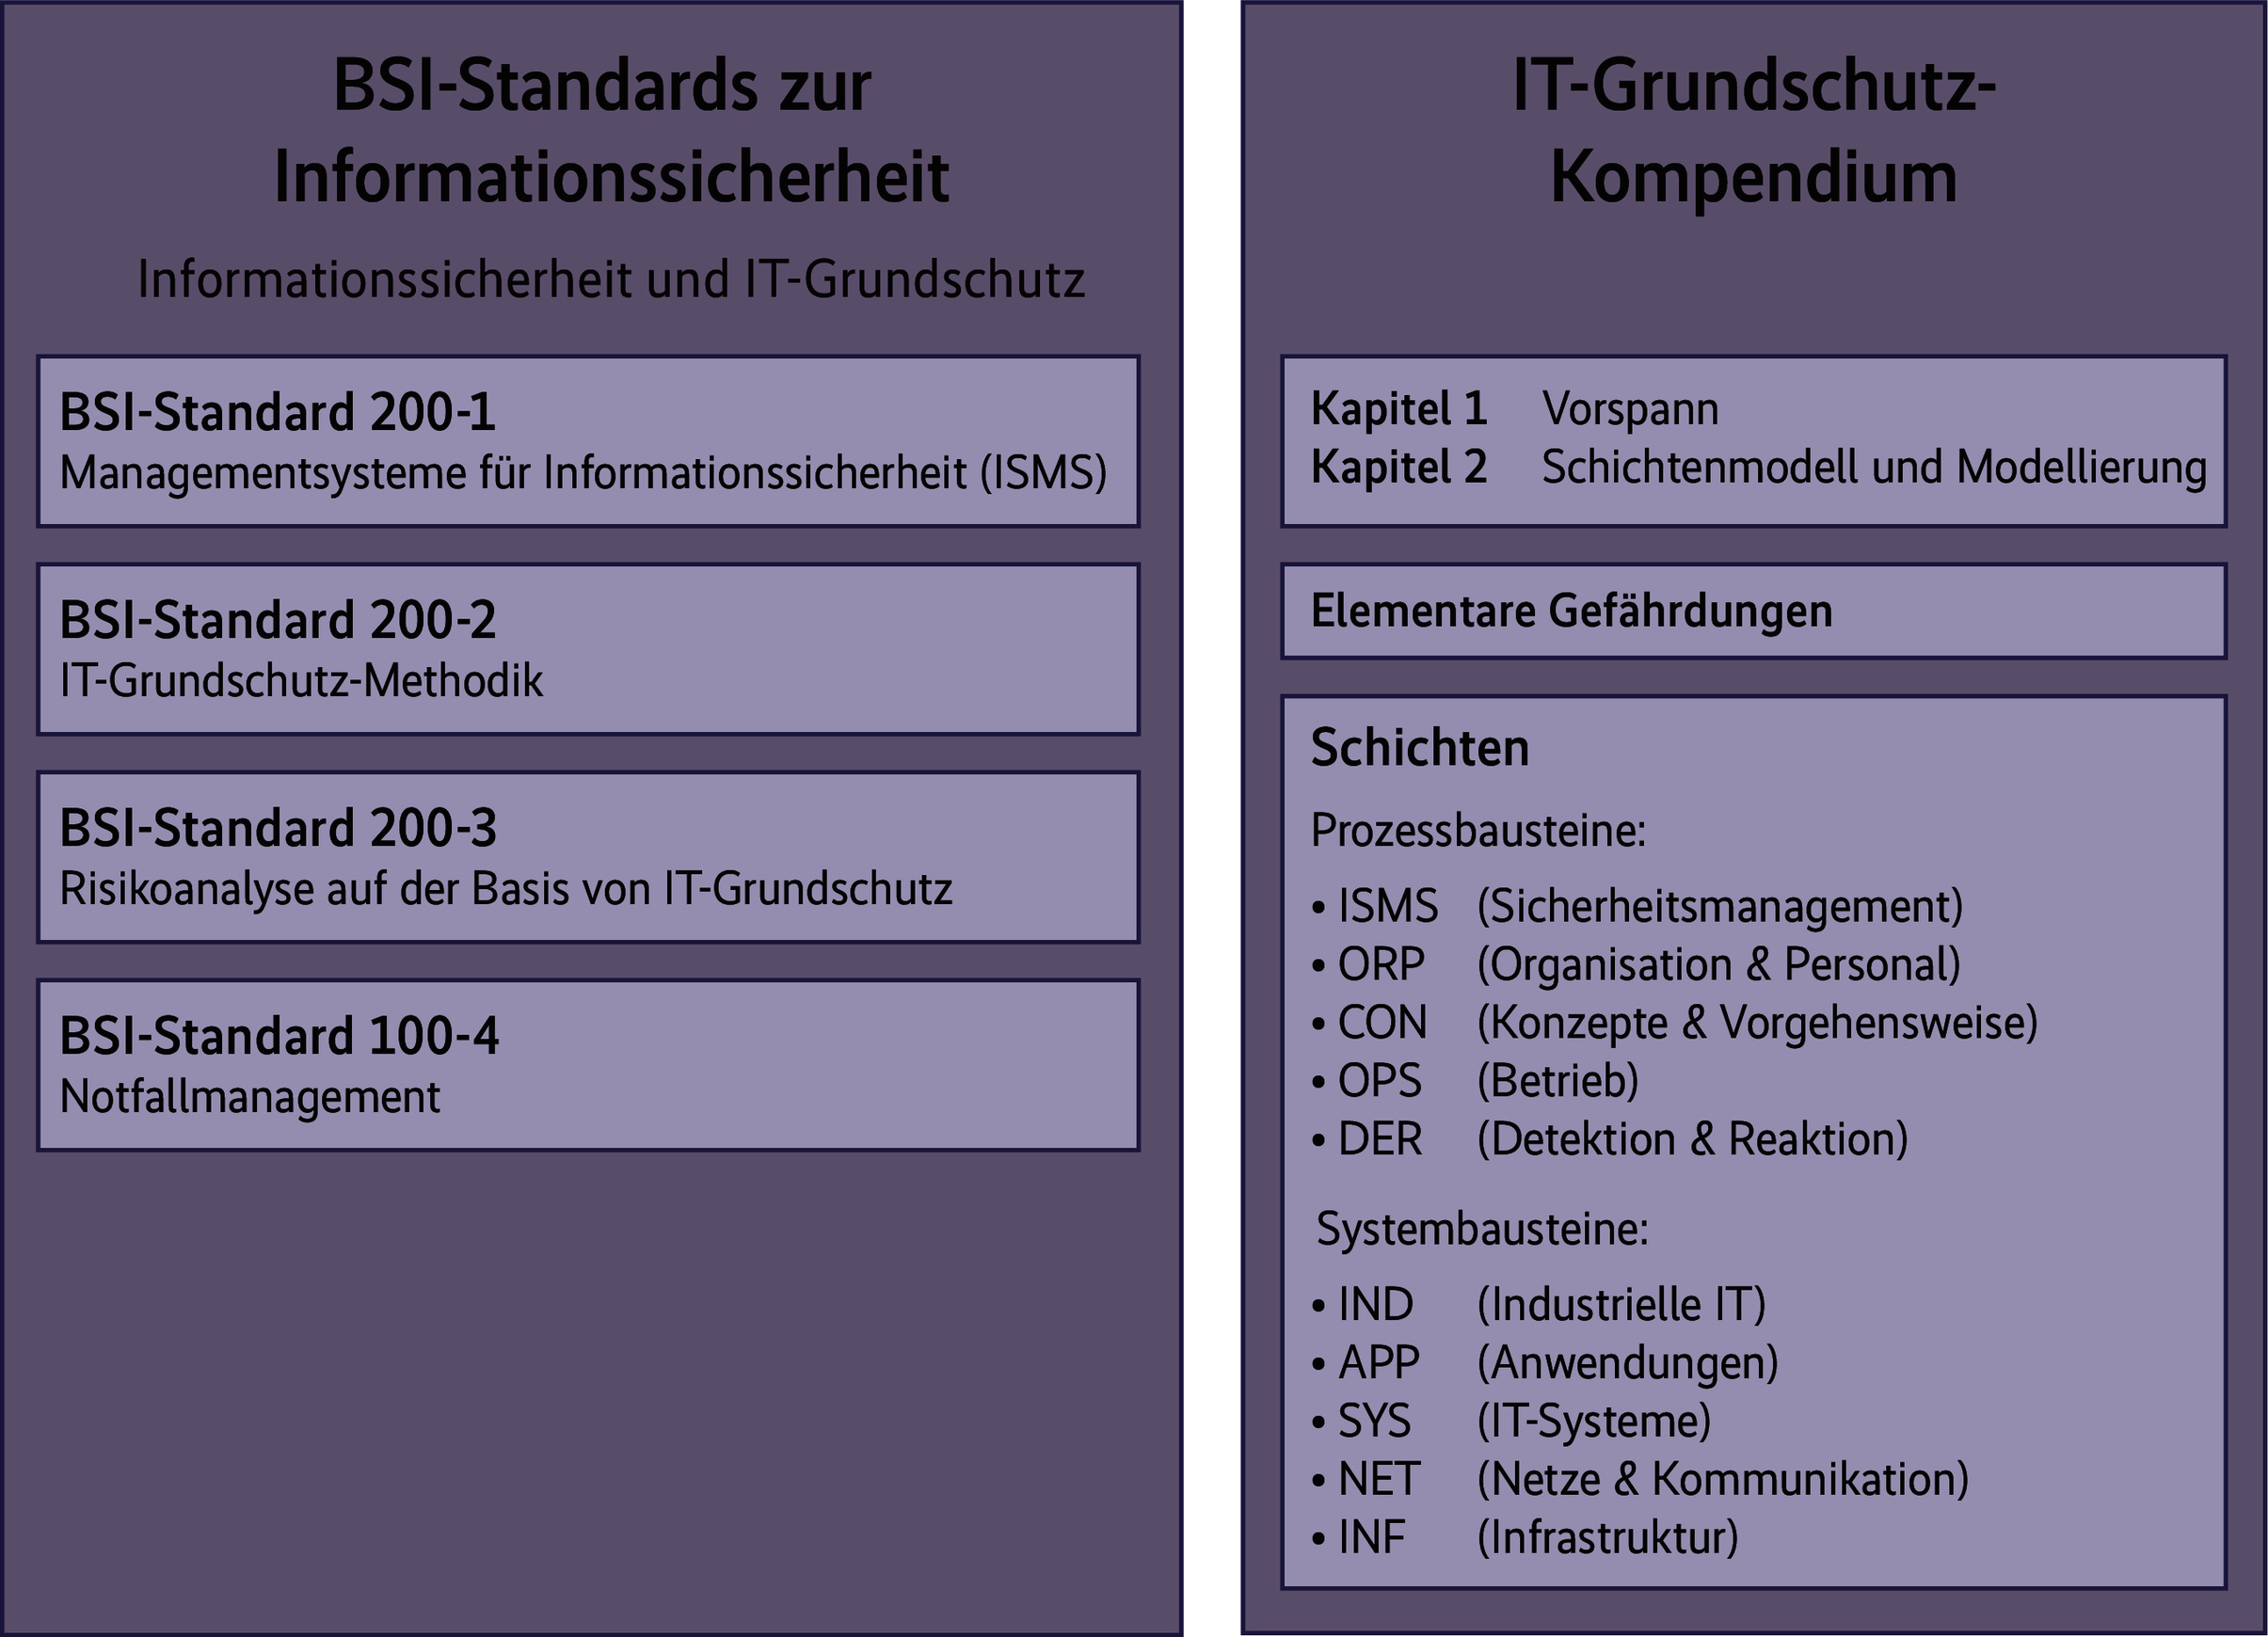
\includegraphics[width=16cm]{images/BSIgrundschutz.png}
    \caption{BSI-Standards und IT-Grundschutz-Kompendium \cite{heise}}
    \label{bsigrundschutz}
    \end{center}
\end{figure}

\paragraph*{BSI-Standard 200-1 - Managementsysteme für Informationssicherheit}\index{BSI-Standards!BSI 200-1}\label{para:BSI 200-1}
\begin{itemize}[noitemsep,topsep=0pt,leftmargin=*]
    \item Zielgruppe: Management
    \item Definiert allgemeine Anforderungen an ein ISMS
    \item Kompatibel mit den entsprechenden Standards der ISO 27000 Reihe
    \item Berücksichtigt insbesondere Empfehlungen aus ISO 13335\index{ISO Standards!ISO 13335} und ISO 27002\index{ISO Standards!ISO 27002}\\({Siehe \underline{\nameref{para:ISO 27002}}, Seite \pageref{para:ISO 27002}})
    \item Didaktisch sehr gut aufbereitet (leicht verständlich)
    \item Enthält diverse Hinweise zur Zusammenarbeit Sicherheitsmanagement und Datenschutz
\end{itemize}

\paragraph*{BSI-Standard 200-2 - IT-Grundschutz-Vorgehensweise}\index{BSI-Standards!BSI 200-2}\label{para:BSI 200-2}
\begin{itemize}[noitemsep,topsep=0pt,leftmargin=*]
    \item Konkretisiert die Darstellung de ISMS nach BSI-Standard 200-1
    \item Beschreibt Aufbau und Betrieb eines ISMS in der Praxis
    \begin{itemize}[noitemsep,topsep=0pt,leftmargin=*]
        \item Aufgaben des IT-Sicherheitsmanagements
        \item Aufbau von Organisationsstrukturen für die Informationssicherheit
    \end{itemize}
    \item Gibt Anleitung
    \begin{itemize}[noitemsep,topsep=0pt,leftmargin=*]
        \item zur Erstellung eine Sicherheitskonzepts
        \item zur Auswahl von angemessenen Sicherheitsmassnahmen
        \item zum Aufrechterhalten und Verbessern der Informationssicherheit
    \end{itemize}
\end{itemize}

\paragraph*{BSI-Standard 200-3 - Risikoanalyse auf Basis von IT-Grundschutz}\index{BSI-Standards!BSI 200-3}\label{para:BSI 200-3}
\begin{itemize}[noitemsep,topsep=0pt,leftmargin=*]
    \item Die Standard-Sicherheitsmassnahmen der IT-Grundschutzkataloge sind in der Regel ausreichend
    \item Es gibt allerdings auch Ausnahmen
    \begin{itemize}[noitemsep,topsep=0pt,leftmargin=*]
        \item Objekte mit besonders hohen Sicherheitsanforderungen
        \item Objekte, welche in den IT-Grundschutzkatalogen nicht behandelt werden
        \item Objekte, welche in Einsatzszenarien betrieben werden, die im Rahmen des IT-Grundschutz nicht vorgesehen sind
    \end{itemize}
    \item In diesen Fällen muss eine Risikoanalyse auf der Basis von IT-Grundschutz durchgeführt werden
\end{itemize}

\begin{figure}[H]
\paragraph*{Risikoanalyse auf Basis von IT-Grundschutz}
    \begin{center}
    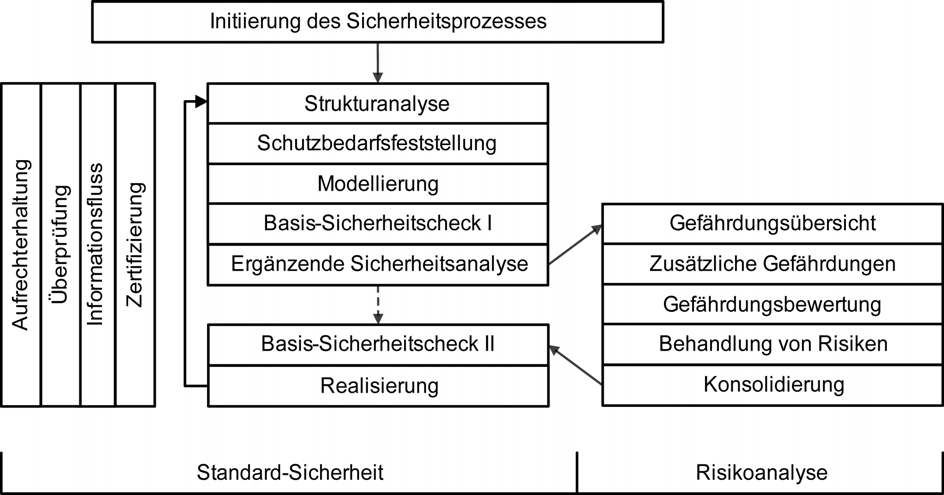
\includegraphics[width=16cm]{images/bsi100-3.png}
    \caption{Standard-Sicherheit und Risikoanalyse}
    \label{bsi100-3}
    \end{center}
\end{figure}

\paragraph*{BSI-Standard 100-4 - Notfallmanagement}\index{BSI-Standards!BSI 100-4}
\begin{itemize}[noitemsep,topsep=0pt,leftmargin=*]
    \item Methodik zur Etabliereung und Aufrechterhaltung eines unternehmensweiten, internen Notfallmanagements
    \item Führt zu einem eigenständigen Managementsystem für die Geschäftsfortführung und Notfallbewältigung
    \item Baut auf der IT-Grundschutzvorgeheinsweise auf (BSI-Standard 100-2)
\end{itemize}
\begin{figure}[H]
    \begin{center}
    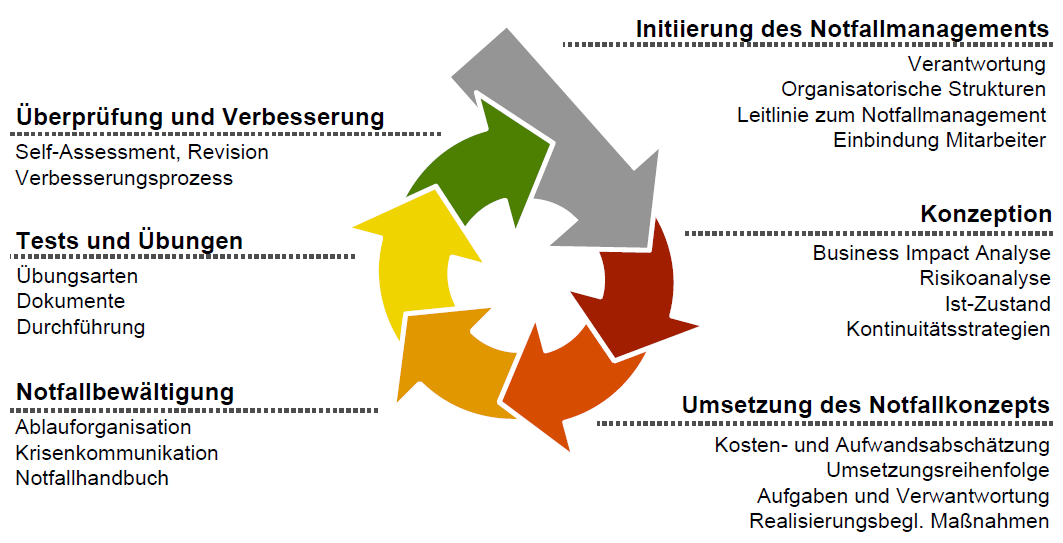
\includegraphics[width=16cm]{images/vortraggrundschutz.png}
    \caption{Iteration des Notfallmanagements nach BSI 100-4 \cite{münch2009}}
    \label{bsi100-4}
    \end{center}
\end{figure}

\subsection*{Sie kennen die Struktur und Grundziele des NIST Cybersecurity Frameworks}\index{NIST Cybersecurity Framework}
\paragraph*{NIST Cybersecurity Framework}\label{para:NIST}Das Cybersecurity Framework ist eine Reihe von Richtlinien für Privatunternehmen, die befolgt werden müssen, um bei den Funktionen Identify, Detect und Respond im Thema Cyberangriffe besser vorbereitet zu sein. Es enthält auch Richtlinien, wie man einen Angriff verhindern und sich von ihm erholen kann.
Einfach ausgedrückt, ist das NIST Cybersecurity Framework eine Reihe von Best~Practices, Standards und Empfehlungen, die einem Unternehmen helfen, seine Cybersicherheitsmassnahmen zu verbessern. Das NIST Cybersecurity Framework versucht, den Mangel an Standards zu beheben, wenn es um Sicherheit geht. Derzeit gibt es grosse Unterschiede in der Art und Weise wie Unternehmen Technologien, Sprachen und Regeln zur Bekämpfung von Hackern, Datenpiraten und Ransomware einsetzen. Die verschiedenen Policies, Guidelines, Best Practices und Technologien, die in der Cybersicherheit verwendet werden, werfen ein weiteres Problem auf: Unternehmen sind nicht in der Lage, Informationen über Angriffe auszutauschen. Aber Vorsicht, das was die andere Firma dagegen getan hat, muss nicht unbedingt für das eigene Unternehmen funktionieren.
Das NIST Cybersecurity Framework zielt darauf ab, all dies zu beseitigen. Mit einem einheitlichen Satz von Regeln, Richtlinien und Standards ist es einfacher, Informationen zwischen zwei Unternehmen auszutauschen und alle auf das gleiche Niveau zu bringen\cite{guardian}.

\paragraph*{Cybersecurity Framework Components}\index{NIST Cybersecurity Framework!Components}\label{para:NISTcomponents}Das NIST Security Framework besteht aus drei Komponenten. Dem Kern (Core), den Umsetzungsebenen (Tiers) und dem Profil (Profile).
\begin{figure}[H]
    \begin{center}
    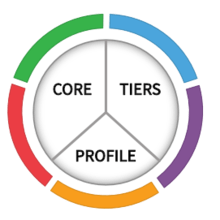
\includegraphics[width=6cm]{images/NISTcomponents.png}
    \caption{Die Komponenten des NIST Frameworks}
    \label{nistcomponents}
    \end{center}
\end{figure}
\textsl{Tiers} und \textsl{Profile} haben wir nicht durchgenommen, weshalb dies nicht weiter beschrieben wird.

\paragraph*{Core}\index{NIST Cybersecurity Framework!Core}\label{para:NISTcore}Der Framework-Kern definiert die Aktivitäten, die Sie durchführen müssen, um unterschiedliche Cybersicherheitsergebnisse zu erzielen. Diese wird in vier verschiedene Elemente unterteilt:
\begin{itemize}[noitemsep,topsep=0pt,leftmargin=*]
    \item Fünf \textbf{Funktionen} für grundlegende Cybersicherheitsaufgaben \footnote{{Siehe \underline{\nameref{nistfunctions}}, Seite \pageref{nistfunctions}}}
    \begin{itemize}[noitemsep,topsep=0pt,leftmargin=*]
        \item Identifizierung
        \item Schutz
        \item Erkennung
        \item Reaktion
        \item Wiederherstellung
    \end{itemize}
    \item Für jede der fünf Funktionen gibt es \textbf{Kategorien}, die eigentlich spezifische Herausforderungen oder Aufgaben sind, welche ausgeführt werden müssen (z.B. Betriebssystem- \& Software-Updates, Antiviren- \& Antimalwareprogramme)
    \item \textbf{Unterkategorien} sind Aufgaben oder Herausforderungen, die mit der Kategorie verbunden sind (z.B. für Betriebssystem-Updates (Kategorie) müssen automatische Updates auf allen Maschinen aktiv sein)
    \item \textbf{Informative Quellen } sind Dokumente \& Handbücher, die spezifische Aufgaben für Benutzer detailliert beschreiben, wie die Dinge durchgeführt werden sollen (z.B. wie automatische Updates aktiviert werden)
\end{itemize}
\textsl{Tiers} und \textsl{Profile} haben wir nicht durchgenommen, weshalb dies nicht weiter beschrieben wird.

\begin{figure}[H]
\paragraph*{Fünf Funktionen der Cybersicherheitsaufgaben}
    \begin{center}
    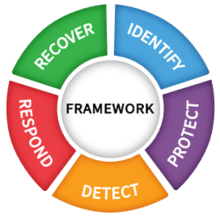
\includegraphics[width=6cm]{images/NISTfunctions.png}
    \caption{Fünf Frameworkfunktionen}
    \label{nistfunctions}
    \end{center}
\end{figure}
\begin{itemize}[noitemsep,topsep=0pt,leftmargin=*]
    \item \textbf{Identifizierungsfunktion} hilft bei der Entwicklung eines organisatorischen Verständnisses für das Management des Cybersicherheitsrisikos für Systeme, Personen, Anlagen, Daten und Fähigkeiten
    \item \textbf{Schutzfunktion} unterstützt die Fähigkeit, die Auswirkungen potenzieller Cybersicherheitsereignisse zu begrenzen oder einzudämmen, und setzt Rahmenbedingungen der Schutzmassnahmen für die Bereitstellung kritischer Dienste
    \item Die \textbf{Erkennungsfunktion} definiert die geeigneten Aktivitäten, um das Auftreten eines Cybersicherheitsereignisses rechtzeitig zu erkennen
    \item Die \textbf{Reaktionsfunktion} umfasst geeignete Aktivitäten, um Maßnahmen in Bezug auf einen erkannten Cybersicherheitsvorfall zu ergreifen und die Auswirkungen zu minimieren
    \item Die \textbf{Wiederherstellungsfunktion} identifiziert geeignete Aktivitäten zur Aufrechterhaltung von Ausfallsicherheitsplänen und zur Wiederherstellung von Diensten, die bei Cybersicherheitsvorfällen beeinträchtigt werden
\end{itemize}


\section{Risiko-Management und IT-Grundschutz}



\subsection*{Sie kennen den Aufbau der IT-Grundschutz-Kataloge und deren Anwendungsweise}
\paragraph*{TODO}







\subsubsection*{Definitionen des Begriffs 'Risiko'}
\index{Risikodefinition}
\begin{itemize}[noitemsep,topsep=0pt,leftmargin=*]
    \item \textbf{Quelle Duden:} \\ Möglicher negativer Ausgang bei einer Unternehmung, mit
    dem Nachteile, Verlust, Schäden verbunden sind; mit einem
    Vorhaben, Unternehmen o. Ä. verbundenes Wagnis.
    \item \textbf{Quelle ISO 27000:2009} \\ Kombination aus der Wahrscheinlichkeit eines Ereignisses und
    dessen Auswirkungen.
    \item \textbf{Quelle: Hans-Peter Königs, IT-RisikoManagement mit System} \\Risiko ist eine Bedrohung, deren Wirkung auf Ziele (SystemZiele) mit Wahrscheinlichkeit (Häufigkeit) und Konsequenz
    bewertet wird. Das Risiko betrachtet dabei die negative,
    unerwünschte und ungeplante Abweichung und deren Folgen
    von System-Zielen
\end{itemize}
\paragraph*{}Hinweis: Dem Risiko kann auch eine positive Abweichung, d.h. eine Chance, gegenüberstehen.

\subsubsection*{Risikomanagement-Stile}
\index{Risikomanagement - Stile}
\begin{figure}[H]
    \begin{center}
    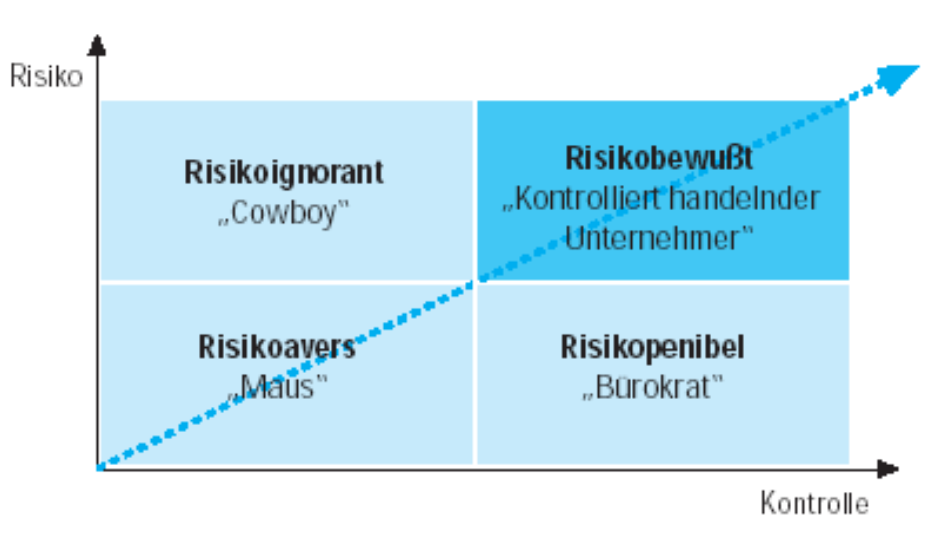
\includegraphics[width=11cm]{images/KPMG_Risikomanagementstile.png}
    \caption{Verschiedene Stile von Risikomanagement}
    \label{risikomanagementstile}
    \end{center}
\end{figure}

\subsubsection*{Unternehmensrisiken}
\index{Risiken Aufzählung}
\begin{figure}[H]
    \begin{center}
    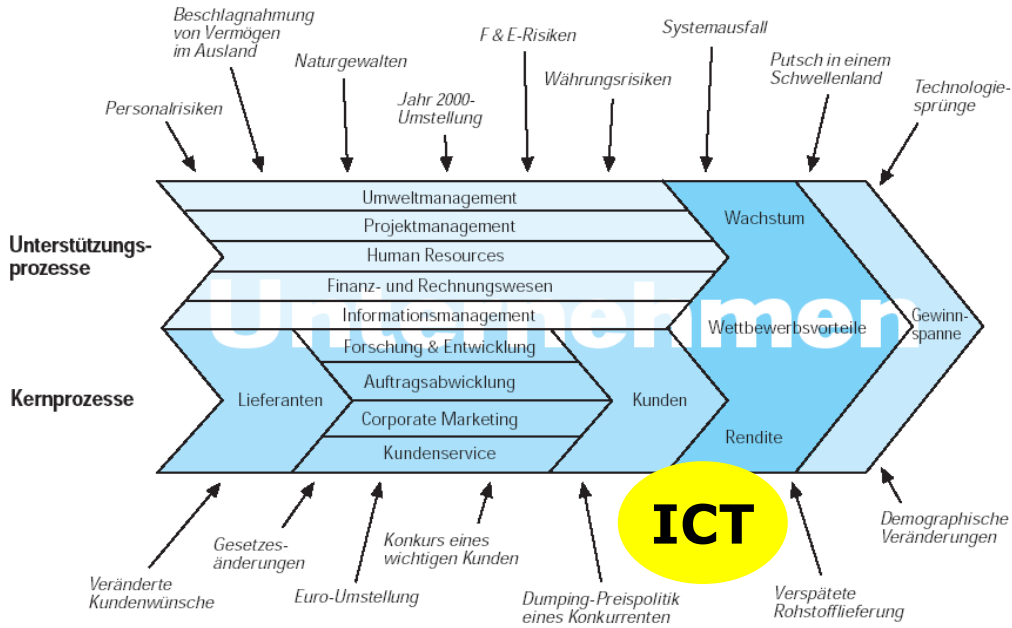
\includegraphics[width=13cm]{images/KPMG_Risiken.png}
    \caption{Risiken laut KPMG}
    \label{KPMG Unternehmensrisiken}
    \end{center}
\end{figure}

\subsubsection*{Risiken im Bereich ICT}

\paragraph*{Organisatorische Risiken:}
\begin{itemize}[noitemsep,topsep=0pt,leftmargin=*]
    \item Nicht autorisierte Zugriffe auf Informationen und
    Applikationen
    \item Nicht prozessbezogener Einsatz von Applikationen
    \item Fehlende Fachkompetenz von Mitarbeitenden
    \item Mangelhafte Testverfahren
    \item Datendiebstahl
\end{itemize}

\paragraph*{Anwendungs- und prozessbezogene Risiken:}
\begin{itemize}[noitemsep,topsep=0pt,leftmargin=*]
    \item Veraltete und nicht integrierte Softwarelösungen
    (Insellösungen)
    \item Fehlende strategische Neuorientierung
\end{itemize}

\paragraph*{Infrastrukturelle Risiken:}
\begin{itemize}[noitemsep,topsep=0pt,leftmargin=*]
    \item IT-Infrastruktur kann den Ansprüchen (z. B.
    Leistungsfähigkeit) nicht gerecht werden
    \item Mangelhaftes Backupkonzept
    \item Fehlender Notfallplan
    \item Fehlender Wiederanlaufsplan (Business Continuity
    Management)
    \item Bauliche oder technische Standards werden nicht erfüllt
    (Schutz vor Zutritt, Feuer und Energieausfall)
    \item Mangelhafte Dokumentation der Systeme
\end{itemize}

\paragraph*{Kostenbezogene Risiken:}
\begin{itemize}[noitemsep,topsep=0pt,leftmargin=*]
    \item Fehlende Kostentransparenz
    \item Mangelhafte Projektdefinition und -organisation mit
    daraus resultierenden Kostenüberschreitungen
\end{itemize}

\paragraph*{Projektbezogene Risiken:}
\begin{itemize}[noitemsep,topsep=0pt,leftmargin=*]
    \item Run-away-Projekte (Zeit, Kosten und Termine laufen aus
    dem Ruder)
    \item Unprofessionelles Projekt-Management
\end{itemize}


\paragraph*{Begriff: Operationelle Risiken} Sämtliche betrieblichen Risiken, welche in einer Unternehmung Schäden verursachen können.
Grosse Bedeutung haben operationelle Risiken im Bankwesen.
\index{Operationelle Risiken}

\subsection*{Das Risikoanalyse-Verfahren verstehen}

\subsubsection*{Bestimmung / Messung von Risiken}

Zugrunde liegende Grössen:
\begin{itemize}[noitemsep,topsep=0pt,leftmargin=*]
    \item \textbf{Eintretenshäufigkeit}
    \item \textbf{Schadensausmass}
\end{itemize}

\index{Risiko Berechnung}
\paragraph*{Risiko = Eintretenshäufigkeit * Schadensausmass}

\subsubsection*{Quantitative vs. qualitative Risiko-Analyse}
\index{quantitative vs. qualitative Risikoanalyse}
\paragraph*{Quantitative Risikoanalyse:}
\begin{itemize}[noitemsep,topsep=0pt,leftmargin=*]
    \item Die an der Risikoanalyse beteiligten Grössen sollen numerisch exakt berechnet werden.
    \item Der monetäre Wert von Assets muss genau bekann sein.
    \item Die Eintrittshäufigkeit muss genau eingeschätzt werden (für Naturkatastrophen gibt es Tabellen, für andere Szenarien ist eine solche Schätzung oft sehr schwierig)
\end{itemize}

\paragraph*{Qualitative Risikoanalyse:}
\begin{itemize}[noitemsep,topsep=0pt,leftmargin=*]
    \item Die an der Risikoanalyse beteiligten Grössen werden anhand einer mehrstufigen Skala nur eingeschätzt, z.B. Schadensausmass '4' auf einer 5-stufigen Skala.
\end{itemize}

\subsubsection*{Vorgehen bei der Risiko-Analyse}
\begin{figure}[H]
    \begin{center}
    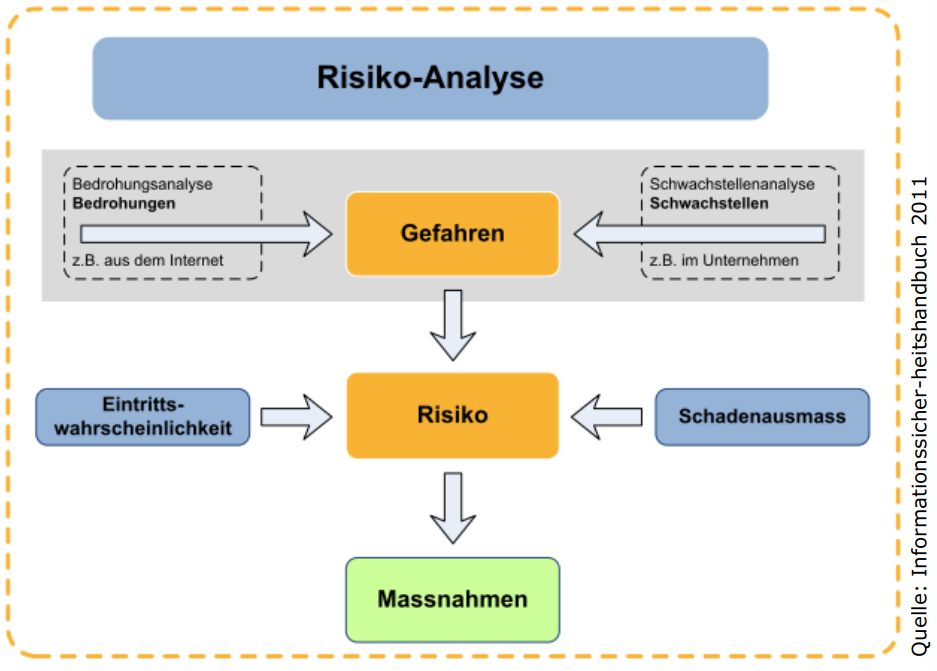
\includegraphics[width=8cm]{images/Risikoanalyse_Vorgehen.png}
    \caption{Vorgehen bei der Risiko-Analyse}
    \label{Risiko-Analyse Vorgehen}
    \end{center}
\end{figure}

\subsubsection*{Bedrohungen nach ISO 27005 (Annex C, 1/3) Citation kap. 8 s.16}\cite{iso27005}
\index{Risiken nach ISO 27005}
\begin{multicols}{2}
[\paragraph*{Phisical damage:}]
\begin{itemize}[noitemsep,topsep=0pt,leftmargin=*]
    \item Fire
    \item Water damage
    \item Pollution
    \item Major accident
    \item Destruction of equipment or media
    \item Dust, corrosion, freezing
\end{itemize}

\paragraph*{Natural events:}
\begin{itemize}[noitemsep,topsep=0pt,leftmargin=*]
    \item Climatic phenomenon
    \item Seismic phenomenon
    \item Volcanic phenomenon
    \item Meteorological phenomenon
    \item Flood
\end{itemize}

\paragraph*{Loss of essential services}
\begin{itemize}[noitemsep,topsep=0pt,leftmargin=*]
    \item Failure of air-conditioning or water
    supply system
    \item Loss of power supply
    \item Failure of telecommunication equipment
\end{itemize}

\paragraph*{Disturbance due to radiation}
\begin{itemize}[noitemsep,topsep=0pt,leftmargin=*]
    \item Electromagnetic radiation
    \item Thermal radiation
    \item Electromagnetic pulses
\end{itemize}

\paragraph*{Compromise of information:}
\begin{itemize}[noitemsep,topsep=0pt,leftmargin=*]
    \item Interception of compromising
    interference signals
    \item Remote spying
    \item Eavesdropping
    \item Theft of media or documents
    \item Theft of equipment
    \item Retrieval of recycled or discarded media
    \item Disclosure
    \item Data from untrustworthy sources
    \item Tampering with hardware
    \item Tampering with software
    \item Position detection
\end{itemize}

\paragraph*{Technical failures:}
\begin{itemize}[noitemsep,topsep=0pt,leftmargin=*]
    \item Equipment failure
    \item Equipment malfunction
    \item Saturation of the information system
    \item Software malfunction
    \item Breach of info system maintainability
\end{itemize}

\paragraph*{Unauthorised actions:}
\begin{itemize}[noitemsep,topsep=0pt,leftmargin=*]
    \item Unauthorised use of equipment
    \item Fraudulent copying of software
    \item Use of counterfeit or copied software
    \item Corruption of data
    \item Illegal processing of data
\end{itemize}

\paragraph*{Compromise of functions:}
\begin{itemize}[noitemsep,topsep=0pt,leftmargin=*]
    \item Error in use
    \item Abuse of rights
    \item Forging of rights
    \item Denial of actions
    \item Breach of personnel availability
\end{itemize}

\paragraph*{Human Threats:}
\begin{itemize}[noitemsep,topsep=0pt,leftmargin=*]
    \item Hacking
    \item Social engineering
    \item System intrusion, break-ins
    \item Unauthorized system access
    \item Computer crime (e.g. cyber stalking)
    \item Fraudulent act (e.g. replay,
    impersonation, interception)
    \item Information bribery
    \item Spoofing
    \item Bomb / Terrorism
    \item Information warfare
    \item System attack (e.g. distributed denial of
    service)
    \item System penetration
    \item System tampering
    \item Defence advantage
    \item Poltical advantage
    \item Economic exploitation
    \item Information theft
    \item Intrusion on personal privacy
    \item Assault on an employee
    \item Blackmail
    \item Browsing of proprietary information
    \item Computer abuse
    \item Fraud and Theft
    \item Input of falsified, corrupted data
    \item Interception
    \item Malicious code (e.g. virus, logic bomb,
    Trojan horse)
    \item Sale of personal information
    \item System bugs
    \item System sabotage
\end{itemize}
\end{multicols}


\subsubsection*{Qualitative Risikoanalyse: Definition Schadensausmass} Es wird empfohlen, eine 3 bis 5-stufige Skale zu definieren, z.B.: \\
\index{Schadensaussmass}
\textbf{Schadensausmass:}
\begin{itemize}[noitemsep,topsep=0pt,leftmargin=*]
    \item \textbf{Vernachlässigbar - Vernachlässigbare Auswirkungen}
    \begin{itemize}[noitemsep,topsep=0pt,leftmargin=*]
        \item Dienstleistung nicht wesentlich gestört
        \item Sachschäden im Bereich von CHF 100.- bis 5'000.-*
        \item keine Verletzten
        \item kein Imageverlust
    \end{itemize}
    \item \textbf{Marginal - Geringe Auswirkungen}
    \begin{itemize}[noitemsep,topsep=0pt,leftmargin=*]
        \item Die Einhaltung gesetzlicher und vertraglicher Pflichten ist nicht gefährdet
        \item Die Dienstleistung sind nur geringfügig beinträchtigt.
        \item Sachschäden im  Bereich von CHF 5000.- bis 50'000.-*
        \item keine Verletzten
        \item kein Imageverlust
    \end{itemize}
    \item \textbf{Kritisch - Grosse Auswirkungen}
    \begin{itemize}[noitemsep,topsep=0pt,leftmargin=*]
        \item Die Einhaltung gesetzlicher und vertraglicher Pflichten ist gefährdet oder die Dienstleistungen sind beeinträchtigt.
        \item Sachschäden im Bereich von CHF 50'000.- bis  500'000.-*
        \item Keine Verletzten
        \item Imageverlust ist klein und von kurzer Dauer
    \end{itemize}
    \item \textbf{Katastrophal - Sehr grosse Auswirkungen}
    \begin{itemize}[noitemsep,topsep=0pt,leftmargin=*]
        \item Die Einhaltung gesetzlicher und vertraglicher Pflichten sind starkk gefährdet oder die Diesntleistungen werden verunmöglicht.
        \item Sachschäden im Bereich \textgreater CHF 500'000.-*
        \item einige Schwerverletzte
        \item grosser Imageschaden (Presse)
    \end{itemize}
\end{itemize}


\subsection*{Eine einfache Risikoanalyse durchführen können}

\subsubsection*{Definition Eintrittshäufigkeit nach Sicherheitshandbuch}
\index{Eintrittshäufigkeit}
Es wird empfohlen, eine 3 bis 5-stufige Skala zu definieren

\begin{itemize}[noitemsep,topsep=0pt,leftmargin=*]
    \item \textbf{Sehr selten}
    \begin{itemize}[noitemsep,topsep=0pt,leftmargin=*]
        \item Möglich aber eher unwahrscheinlich \\z.B. 1-mal in 10 Jahren
    \end{itemize}
    \item \textbf{Selten}
    \begin{itemize}[noitemsep,topsep=0pt,leftmargin=*]
        \item Tritt selten ein, aber kann vorkommen\\z.B. alle 5 Jahre
    \end{itemize}
    \item \textbf{Oft}
    \begin{itemize}[noitemsep,topsep=0pt,leftmargin=*]
        \item Tritt gelegentlich ein\\z.B. jährlich
    \end{itemize}
    \item \textbf{Sehr oft}
    \begin{itemize}[noitemsep,topsep=0pt,leftmargin=*]
        \item Kommt öfters vor\\z.B. monatlich
    \end{itemize}
\end{itemize}

\subsubsection*{Qualitative Risikoanalyse: Risikomatrix}
\index{Risikomatrix}
\begin{figure}[H]
    \begin{center}
    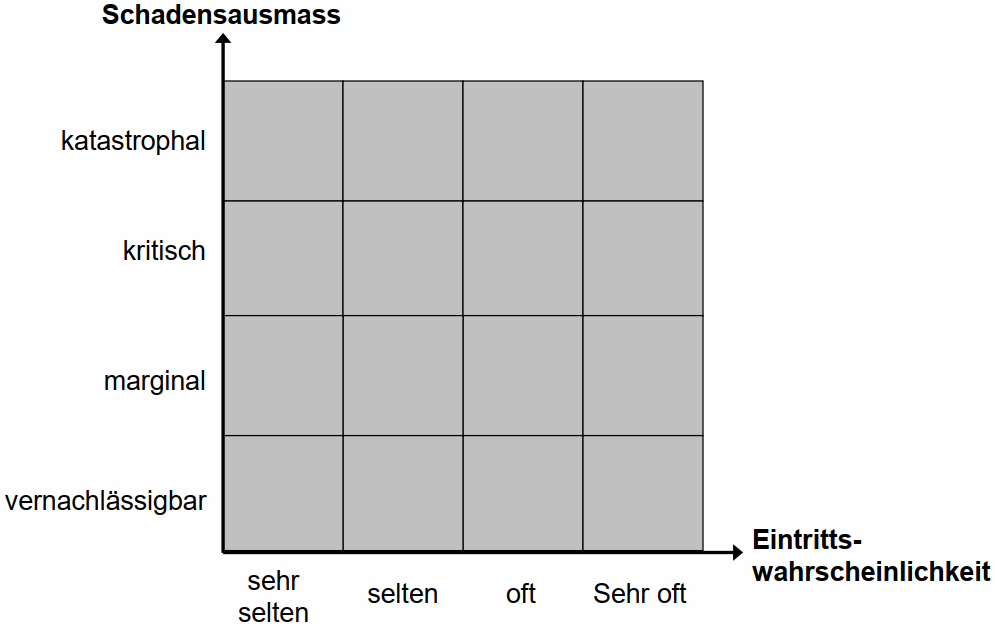
\includegraphics[width=11cm]{images/Risikomatrix.png}
    \caption{Risikomatrix}
    \label{Risikomatrix}
    \end{center}
\end{figure}

\subsubsection*{Risiko-Portfolio, Risiko-Landkarte (Risk-Map)}
\index{Risk-Map}
\index{Risiko-Portfolio}
\begin{itemize}[noitemsep,topsep=0pt,leftmargin=*]
    \item Eine Menge von risiken, welche im Rahmen einer Risikoanalyse identifiziert worden ist, wird als \textbf{Risiko-Portfolio} bezeichnet.
    \item Risiko-Portfolios werden oft einzelnen Geschäftsfeldern zugeordnet (jedes Geschäftsfeld hat sein Portfolio)
    \item Werden die Einzelrisiken des Portfolios in einer Risikomatrix eingezeichnet, so spricht man von einer \textbf{Risiko-Landkarte (Risk-Map)}
\end{itemize}

\begin{figure}[H]
    \begin{center}
    \includegraphics[width=8cm]{images/Risikobewältigung.png}
    \caption{Risk-Map}
    \label{Risk-Map}
    \end{center}
\end{figure}

\begin{figure}[H]
    \begin{center}
    \includegraphics[width=8cm]{images/Risikobewältigung2.png}
    \caption{Risk-Map2}
    \label{Risk-Map2}
    \end{center}
\end{figure}

\subsubsection*{Umgang mit Risiken / Risikobewältigung }
\index{Risikobewältigung}
\index{Restrisiken}
\begin{itemize}[noitemsep,topsep=0pt,leftmargin=*]
    \item \textbf{Risiken vermeiden:}\\Anpassen oder aufgeben von Geschäftsprozessen, sodass die Risiken nicht mehr vorhanden sind.
    \item \textbf{Risiken vermindern:}\\Mit geeigneten Sicherheitsmassnahmen das Schadensausmass oder die Eintrittshäufigkeit reduzieren.
    \item \textbf{Risiken übertragen (transferieren):}\\Überwälzung finanzieller Schäden auf Versicherungen, Outsourcer doer Benutzer einers Service.
    \item \textbf{Risiken tragen:}\\Akzeptieren von Risiken (Restrisiken)
\end{itemize}

\begin{figure}[H]
    \begin{center}
    \includegraphics[width=13cm]{images/Risikobewältigung3.png}
    \caption{Umgang mit Risiken}
    \label{Umgang mit Risiken}
    \end{center}
\end{figure}
\noindent
Der Entscheid, wie mit Risiken umgegangen werden soll, muss dokumentiert und von der Geschäftsleitung genehmigt werden.\\Das Gleiche gilt insbesondere auch für die verbleibenden Restrisiken.
\index{Risiko-Katalog}
\index{Risk Register}
\begin{figure}[H]
    \begin{center}
    \includegraphics[width=10cm]{images/Risiko-Katalog.png}
    \caption{Beispiel eines Risikokataloges}
    \label{risikokatalog}
    \end{center}
\end{figure}

\subsubsection*{Auswahl von Massnahmen zur Risikoreduktion}
\begin{itemize}[noitemsep,topsep=0pt,leftmargin=*]
    \item Welche Massnahmen haben die grösste Wirkung
    (Reduktion mehrerer Risiken)?
    \item Welche Massnahmen benötigen wenig Ressourcen?
    \item Welche Massnahmen können kurzfristig realisiert
    werden?
    \item Welche Massnahmen stossen auf breite Akzeptanz?
\end{itemize}
\noindent
Wirtschaftlichkeit und den Faktor Mensch nie ausser Acht lassen!

\subsubsection*{Risiko-Management-Prozess}
\index{Risiko-Management-Prozess}
\begin{figure}[H]
    \begin{center}
    \includegraphics[width=14cm]{images/Risiko_Management_Prozess.png}
    \caption{Organisation eines Risiko Managements}
    \label{Risiko Management Prozess}
    \end{center}
\end{figure}

\begin{itemize}[noitemsep,topsep=0pt,leftmargin=*]
    \item \textbf{Context Establishment:}\\Gegenstand, Zweck, Absichten,
    Ziele, Fokus und relevante Einflüsse, Randbedingungen und
    Abgrenzungen aus externer und interner Sicht festlegen
    \begin{itemize}[noitemsep,topsep=0pt,leftmargin=*]
        \item wichtige Ziele der Geschäfts- und Support-Prozesse
        \item „Risiko- und Sicherheitspolitik“ für wichtigste Kontext-Elemente
        \item für wen stehen Risiken zur Behandlung an und für wen/was wird das Risiko-Management durchgeführt (z.B. Anspruchsgruppen)?
        \item Gesetzliche, regulatorische und vertragliche Anforderungen
        \item Für das Risikomanagement massgebliche Führungs-Aspekte, organisatorische Festlegungen und Verantwortlichkeiten sowie Berichtserstattungs- und Eskalations-Wege
        \item Anzuwendender Risiko-Management-Ansatz
        \item Schnittstellen zum Corporate Risikomanagement (z.B. Op-Risk)
        \item Risiko-Arten und System-Ziele (z.B. Prozessrisiken, Verfügbarkeits- und Integritätsanforderungen)
        \item Impact Kriterien (Schadensmetrik)
        \item Bewertungskriterien und –massstäbe (z.B. Risiko-Matrix, Dringlichkeitsstufe)
        \item Akzeptanzkriterien (z.B. Akzeptanzlinie)
        \item Dokumentationsvorgaben
    \end{itemize}
    \item \textbf{Risk Identification:}\\Objekte, Bedrohungen,
    Schwachstellen und bereits existierende Massnahmen
    erfassen
    \begin{itemize}[noitemsep,topsep=0pt,leftmargin=*]
        \item Erfassung der Assets (Risiko-Objekte)
        \item vollständigen Erfassung der Gefahrenquellen und der Aufsuchen bereits existierender Massnahmen
        \item Identifikation der vorhandenen Vulnerabilities (Schwachstellen)
        \item Relevante Kausalketten (Ursachen/Wirkungen und Konsequenzen) zusammenstellen
    \end{itemize}
    \item \textbf{Risk Estimation:}\\Häufigkeit und Schadensausmass
    einschätzen
    \begin{itemize}[noitemsep,topsep=0pt,leftmargin=*]
        \item \textbf{Teil-Analysen:}
        \item Impact-Analyse (Analyse der potentiellen Schäden)
        \item Bedrohungs-Analyse (Analyse der relevanten Bedrohungen)
        \item Schwächen-Analyse (Analyse der relevanten Schwachstellen)
        \item Beliebige Kombination der Analysen 1 bis 3
        \item Qualitative oder quantitative Risiko-Analyse
        \item Semi-quantitative Analyse
    \end{itemize}
    \item \textbf{Risk Evaluation:}\\Bewertung der identifizierten Risiken im
    definierten Kontext (Bsp. zeitl. Prioritäten für die
    Umsetzung von Massnahmen; Reduktion Häufigkeit oder
    Schadensausmass?; Abwägung Risiken/Chancen etc.)
    \begin{itemize}[noitemsep,topsep=0pt,leftmargin=*]
        \item Bewertung im Kontext des Untersuchungs- und Behandlungs-Gegenstands (Vergleich mit den im Kontext definierten Kriterien, z.B. Risiko-Toleranz)
        \item Reduktion Häufigkeit oder Schadensausmass?
        \item Für Massnahmen relevante zusätzliche Anforderungen, z.B. vertragliche, gesetzliche, regulatorische Anforderungen, Standards, Qualitäts- und Leistungsanforderungen, Zeit- und Kostenbeschränkungen
        \item Risiken / Chancen abwägen hinsichtlich Optimum
        \item Risiko-Wahrnehmung der Umgebung und des Managements einbeziehen
        \item Risiken mit Attributen versehen: z.B. „wichtig“, „dringlich“ oder „beobachten“
        \item Entscheid über allenfalls notwendige Nachbesserung der Assessment-Ergebnisse
    \end{itemize}
    \item \textbf{Risk Treatment:}\\Definition, Konzeption, Planung und
    Umsetzung von Massnahmen aufgrund der bei der
    Risk Evaluation definierten Anforderungen (Varianten:
    vermeiden, vermindern, transferieren, tragen)
    \begin{itemize}[noitemsep,topsep=0pt,leftmargin=*]
        \item Berücksichtigung Anforderungen an Massnahmen
        \item Auswahl von Massnahmen mit Hilfe von ISO/IEC 27002
        \item Machbarkeit der Massnahmen
        \item Bewältigungs-Optionen-Wahl:
        \item Risiken vermeiden, z.B. durch Aufgabe risikoreicher Aktivitäten
        \item Risiken reduzieren, durch Reduktion entweder der Eintritts-Wahrscheinlichkeit oder des Schadensausmasses
        \item Risiken transferieren, z.B. Überwälzung finanzieller Schäden auf Versicherungen
        \item Risiken bewusst eingehen und tragen,  z.B. Tragen des Restrisikos, welches im Rahmen der betrieblichen Reserven und eines allfälligen Goodwill-Verlusts verkraftbar ist
        \item Abwägen Risiken mit Massnahmenkosten
        \item Kosten-/Nutzen-Untersuchungen
        \item Umsetzungsplan
    \end{itemize}
    \item \textbf{Risk Acceptance:}\\Formaler Akzept des Risk
    Treatment Plans sowie der Restrisiko-Einschätzung
    durch das zuständige Management
    \begin{itemize}[noitemsep,topsep=0pt,leftmargin=*]
        \item Bewältigungsplan (mit Verantwortlichkeiten und Terminen) sowie Restrisiko-Einschätzung müssen durch das zuständige Management formal akzeptiert sein
        \item Restrisiken, die nach der Bewältigung die Akzeptanz-Kriterien nicht erfüllen, müssen schriftlich begründet und durch das zuständige Management schriftlich zur Kenntnis genommen und akzeptiert werden.
        \item Massnahmen-Überwachung, -Überprüfung Erneute Risiko-Einschätzung und –Bewertung aufgrund veränderter Situation
        \item Wiederholung im Rahmen eines jährlichen Risikoberichts (z.B. synchron zum rollierenden Strategieprozess)
    \end{itemize}
    \item \textbf{Risk Communication:}\\Information der direkt
    Beteiligten und der Betroffenen in jedem Teilprozess
    \begin{itemize}[noitemsep,topsep=0pt,leftmargin=*]
        \item Kommunikation mit Beteiligten und Betroffenen (z.B. Anspruchsgruppen)
        \item angemessene Kommunikation unter Fachpersonen, Experten, Entscheidungsträgern und Anspruchsgruppen
        \item Berücksichtigung der Risiko-Wahrnehmung
        \item Stärkung des Risiko-Bewusstseins
        \item Einsatz „stark strukturierter“ Kommunikationsformen
        \item Kommunikations-Konzept für Risiko-Kommunikation im Normalbetrieb, für risikorelevante Ereignisse und in Notfallsituationen
    \end{itemize}
    \item \textbf{Risk Monitoring and Review:}\\Prozess und RisikoSituation bezüglich allfälliger Veränderungen
    überwachen
    \begin{itemize}[noitemsep,topsep=0pt,leftmargin=*]
        \item Prozess und Risiko-Situation überwachen (z.B. Überwachung Änderungs-Prozesse, Entwicklungsprozesse und Betriebsprozesse)
        \item Überwachung mit Risiko-Indikatoren und mit Frühwarnsystem
        \item Registrierung von Veränderungen von Kontext und Risikosituation sowie Verbesserungs-Empfehlungen hinsichtlich Risikomanagement sowie aktueller und zukünftiger Risikosituation aufzeigen
        \item Überprüfung durch unabhängige Auditoren
        \item Verifikation anhand Reifegradmodell
        \item Risiko-Berichte
        \item Unabhängigkeit der Berichterstattung
    \end{itemize}
\end{itemize}

\paragraph*{Kriterien für die Prozesswiederholung:}
\begin{itemize}[noitemsep,topsep=0pt,leftmargin=*]
    \item \textbf{Externer Trigger:}\\Sich ändernde
    Umgebungsbedingungen; inakzeptable Restrisiken
    aufgrund ungenügend realisierter Massnahmen; neue
    regulatorische Anforderungen
    \item \textbf{Periodische Durchführung:}\\Synchron mit anderen
    Management-Prozessen (z. B. Strategieprozess)
\end{itemize}

\subsubsection*{Verfahren für den Umgang mit Risiken}
\begin{figure}[H]
    \begin{center}
    \includegraphics[width=8cm]{images/Schutzbedarf.png}
    \caption{Schutzbedarf}
    \label{Schutzbedarf}
    \end{center}
\end{figure}

\begin{itemize}[noitemsep,topsep=0pt,leftmargin=*]
    \item Grundschutz (z.B. gemäss BSI)
    \begin{itemize}[noitemsep,topsep=0pt,leftmargin=*]
        \item Stadardisierte Massnahmen
        \item Generelle Risikobetrachtung
    \end{itemize}
    \item Risikoanalyse
    \begin{itemize}[noitemsep,topsep=0pt,leftmargin=*]
        \item Spezifische Massnahmen
        \item Detaillierte Risikobetrachtung
    \end{itemize}
    \item Kombinierter Ansatz (zweistufiges Vorgehen, z.B. gemäss BSI)
    \begin{itemize}[noitemsep,topsep=0pt,leftmargin=*]
        \item Grundschutz bei Schutzbedarf klein und mittel
        \item Risikoanalyse bei schutzbedarf hoch und sehr hoch
    \end{itemize}
\end{itemize}


\subsubsection*{Kombinierter Ansatz: Grundschutz und Risikoanalyse}
\index{Kombinierter Ansatz}
\begin{figure}[H]
    \begin{center}
    \includegraphics[width=8cm]{images/Kombinierter_Ansatz.png}
    \caption{Kombinierter Ansatz}
    \label{Kombinierter Ansatz}
    \end{center}
\end{figure}

\subsubsection*{BSI-Standard 200-3: Risikoanalyse auf Basis von IT-Grundschutz}
\index{BSI-Standards!BSI 200-3}
\begin{figure}[H]
    \begin{center}
    \includegraphics[width=8cm]{images/BSI200-3.png}
    \caption{BSI-Standard 200-3}
    \label{BSI-Standard 200-3}
    \end{center}
\end{figure}

\subsubsection*{IT-Grundschutz-kataloge}
\index{Grundschutz - IT Grunschutz}
\begin{figure}[H]
    \begin{center}
    \includegraphics[width=8cm]{images/IT-Grundschutz-Kataloge.png}
    \caption{IT-Grundschutz-Kataloge}
    \label{IT-Grundschutz-Kataloge}
    \end{center}
\end{figure}


\subsection*{Die Unterschiede zum Grundschutzverfahren kennen}
\paragraph*{Bemerkungen zu den IT-Grundschutz-Katalogen}
\begin{itemize}[noitemsep,topsep=0pt,leftmargin=*]
    \item Die Beschreibung der Gefährdungen dient lediglich
    der Sensibilisierung und der Begründung von
    Massnahmen und hat im Grundschutz-Vorgehen keine
    weitere Funktion!
    \item Das BSI macht keine Unterscheidung zwischen
    Gefahren und Schwachstellen!
    \item Die Inhalte haben Empfehlungscharakter und sind
    keine 'Gesetze'!
    \item Es gibt keine Garantie auf Vollständigkeit!
    \item IT-Grundschutz-Massnahmen müssen gegebenenfalls
    individuell angepasst und angewendet werden!
\end{itemize}

\subsection*{Sie verstehen die Idee, die Ziele und die Konzepte des IT-Grundschutz-Vorgehens}

\paragraph*{IT-Grundschutz Wirkungsprinzip} Gilt generell, unabhängig vom angwendeten Standard, also nicht nur für den BSI IT-Grundschutz!
\index{IT-Grundschutz}
\begin{figure}[H]
    \begin{center}
    \includegraphics[width=8cm]{images/Grundschutz_Wirkprinzip.png}
    \caption{IT-Grundschutz Wirkprinzip}
    \label{IT-Grundschutz Wirkprinzip}
    \end{center}
\end{figure}

\paragraph*{Grundregeln beim Vorgehen nach IT-Gruzndschutz}
\begin{itemize}[noitemsep,topsep=0pt,leftmargin=*]
    \item Die Initiative für IT-Sicherheit geht vom Management
    aus
    \item Die Verantwortung für IT-Sicherheit liegt beim
    Management
    \item Nur wenn sich das Management um
    Informationssicherheit bemüht, wird die Aufgabe auch
    wahrgenommen
\end{itemize}

\paragraph*{Erstellung eines IT-Sicherheitskonzepts} Der blau hinterlegte Bereich beschreibt diejenigen Schritte, welche notwendig sind, um einen IT-Grundschutz zu etablieren. Als Resultat des erstellten IT-Grundschutzes liegt ein Sicherheitskonzept vor.
\index{IT-Sicherheitskonzept}
\begin{figure}[H]
    \begin{center}
    \includegraphics[width=11cm]{images/IT_Sicherheitskonzept.png}
    \caption{IT Sicherheitskonzept}
    \label{IT Sicherheitskonzept}
    \end{center}
\end{figure}

\paragraph*{IT-Grundschutz - Pro Argumente}
\begin{itemize}[noitemsep,topsep=0pt,leftmargin=*]
    \item Standardbasierend
    \item Vollständigkeit der \textbf{Massnahmenpakete}
    \item Keine detaillierte Risikoanalyse notwendig
    \item Gleichmässiger, umfassender Schutz auf
    allen Objekten
    \item Einfach und schnell anwendbar
    \item Definierte Basis für weitergehende
    Schutzmassnahmen (ergänzende
    Sicherheitsanalyse)
\end{itemize}

\paragraph*{Achtung beim IT-Grundschutz!!}
\begin{itemize}[noitemsep,topsep=0pt,leftmargin=*]
    \item Ungenügender Schutz bei erhöhten Risiken
    oder besonderem Schutzbedarf
    \item Mögliche Einschränkung der Funktionalität
    durch Überschutz
    \item Begründung von Massnahmen schwierig
    \item Je nach Detaillierungsgrad, Anspruch an
    Aktualität und Vollständigkeit des
    Massnahmenkataloges aufwändig
    \item Vorteile des Grundschutzvorgehens nicht
    durch administrativen 'Overkill' zunichte
    machen
\end{itemize}

\subsubsection*{Kreuzreferenztabellen}
\index{Kreuzreferenztabellen}
\begin{figure}[H]
    \begin{center}
    \includegraphics[width=8cm]{images/Kreuzreferenztabellen.png}
    \caption{Kreuzreferenztabellen}
    \label{Kreuzreferenztabellen}
    \end{center}
\end{figure}

\paragraph*{Kreuzreferenztabellen:}Tabellen, welche angeben, welchen Gefährdungen mit welchen Massnahmen begegnet werden kann (bezogen auf einen bestimmten Baustein)

\begin{itemize}[noitemsep,topsep=0pt,leftmargin=*]
    \item Die Massnahmen werden priorisiert (sog. Siegelstufe)
    \begin{itemize}[noitemsep,topsep=0pt,leftmargin=*]
        \item \textbf{A:} Essenzielle massnahme, vorrangig umzusetzen
        \item \textbf{B:} Besonders wichtige massnahme, zügig umsetzen
        \item \textbf{C:} Wichtige Massnahme, verzögerte Umsetzung zulässig
        \item \textbf{Z:} Ergänzende Massnahme, Umsetzung nicht zwingend notwendig
    \end{itemize}
    \item Wichtig:
    \begin{itemize}[noitemsep,topsep=0pt,leftmargin=*]
        \item Anzahl 'X' ist kein Mass für die Wichtigkeit einer Massnahme
        \item Nur die wichtigsten Gefährdungen sind aufgeführt
    \end{itemize}
\end{itemize}


%wenn möglich neue Seite
\subsection*{Sie können die Teilschritte zum Aufbau eines Sicherheitskonzeptes nach IT-Grundschutz durchführen, kombinierte Risikoanalyse}

\subsubsection*{IT-Strukturanalyse}
\index{Strukturanalyse}
\begin{figure}[H]
    \begin{center}
    \includegraphics[width=6cm]{images/Strukturanalyse.png}
    \caption{IT-Strukturanalyse}
    \label{IT-Strukturanalyse}
    \end{center}
\end{figure}

\paragraph*{IT-Strukturanalyse - Erhebung Netzwerkplan}

\begin{itemize}[noitemsep,topsep=0pt,leftmargin=*]
    \item Netzwerkplan |\textsl{aktualisieren}
    \begin{itemize}[noitemsep,topsep=0pt,leftmargin=*]
        \item Netzwerkpläne sind meist nicht auf dem
        aktuellsten Stand
        \item Entsprechende Informationen beschaffen bei
        IT-Verantwortlichen, Administratoren resp.
        Netz- und Systemmanagement
    \end{itemize}
    \item Netwerkplan \textsl{auserten}
    \begin{itemize}[noitemsep,topsep=0pt,leftmargin=*]
        \item  Welche IT-Systeme gibt es? (Clients, Server,
        Netzwerk-Komponenten etc.)
        \item Welche Verbindungen zw. diesen Systemen?
        \item Welche Verbindungen nach aussen (Einwahl,
        Internet, VPN etc.)
    \end{itemize}
\end{itemize}

\paragraph*{IT-Strukturanalyse - Komplexitätsreduktion}
\begin{itemize}[noitemsep,topsep=0pt,leftmargin=*]
    \item Gleichartige Komponenten zu Gruppen
    zusammenfassen
    \item Mögliche Gruppierungskriterien
    \begin{itemize}[noitemsep,topsep=0pt,leftmargin=*]
        \item Systeme von gleichem Typ
        \item Systeme mit gleicher oder nahezu gleicher Konfiguration
        \item Systeme mit gleicher oder nahezu gleicher
        Netzwerkanbindung
        \item Systeme mit gleichen administrativen und
        infrastrukturellen Rahmenbedingungen
        \item Systeme, welche für gleiche Aufgaben genutzt werden
        \item Systeme, welche den gleichen Schutzbedarf aufweisen
    \end{itemize}
    \item Die bei der Komplexitätsreduktion entstandenen
    Gruppen werden fortan wie einzelne Objekte
    behandelt
    \item Wichtig: Keine Komponenten mit zu
    unterschiedlichem Schutzbedarf zusammen fassen,
    Beispiele:
    \begin{itemize}[noitemsep,topsep=0pt,leftmargin=*]
        \item Clients der Geschäftsleitung nicht in Gruppe der
        'normalen' Clients integrieren
        \item Dito für Clients von Entwicklungsabteilung,
        Personalabteilung, Buchhaltung und IT-Administration
        \item Sie alle haben einen erhöhten Schutzbedarf
    \end{itemize}
\end{itemize}

\paragraph*{}Beispiel für das Resultat einer Komplexitätsreduktion (Gruppen gleichartiger Komponenten)
\begin{figure}[H]
    \begin{center}
    \includegraphics[width=12cm]{images/Komplexitätsreduktion.png}
    \caption{Komplexitätsreduktion}
    \label{Komplexitätsreduktion}
    \end{center}
\end{figure}

\paragraph*{IT-Strukturanalyse –Erhebung IT-Systeme}
\begin{figure}[H]
    \begin{center}
    \includegraphics[width=10cm]{images/Erhebung IT-Systeme.png}
    \caption{Erhebung IT-Systeme}
    \label{Erhebung IT-Systeme}
    \end{center}
\end{figure}

\paragraph*{IT-Strukturanalyse - Zuordnung von Systemen und Anwendungen}
\begin{itemize}[noitemsep,topsep=0pt,leftmargin=*]
    \item Der Schutzbedarf eines IT-Systems hängt vom
    Schutzbedarf der Anwendungen ab, welche es
    unterstützt
    \item IT-Systeme (Server, Clients) und Anwendungen
    werden einander deshalb zugeordnet
\end{itemize}
\begin{figure}[H]
    \begin{center}
    \includegraphics[width=10cm]{images/Zuordnung_Sys_App.png}
    \caption{Zuordnung in Gruppen}
    \label{Zuordnung in Gruppen}
    \end{center}
\end{figure}

\begin{itemize}[noitemsep,topsep=0pt,leftmargin=*]
    \item Für den Schutzbedarf eines Systems ist diejenige
    Anwendung mit den höchsten
    Sicherheitsanforderungen (bezüglich Vertraulichkeit,
    Integrität und Verfügbarkeit) relevant
    \item Es gilt das sog. Maximumprinzip (vgl. zugehörige
    Folien)
\end{itemize}

\subsubsection*{Schutzbedarfsfeststellung}
\index{Schutzbedarsfestellung}
\begin{figure}[H]
    \begin{center}
    \includegraphics[width=6cm]{images/Schutzbedarfsfeststellung.png}
    \caption{Schutzbedarfsfeststellung}
    \label{Schutzbedarfsfeststellung}
    \end{center}
\end{figure}

\paragraph*{Schutzbedarfsfeststellung - Ziel}
\begin{itemize}[noitemsep,topsep=0pt,leftmargin=*]
    \item Bestimmung des Schutzbedarfs des
    betrachteten Informationsverbunds
    \item Zu beantwortende Fragen:
    \begin{itemize}[noitemsep,topsep=0pt,leftmargin=*]
        \item Wie viel Schutz benötigen die identifizierten
        Objekte?
        \item Wie kommt man zu einer begründeten und
        nachvollziehbaren Einschätzung des
        Schutzbedarfs?
        \item Welche Objekte haben einen erhöhten
        Schutzbedarf?
    \end{itemize}
\end{itemize}

\begin{multicols}{2}[\paragraph*{Schutzbedarfsfeststellung–Vorgehen}]
\begin{itemize}[noitemsep,topsep=0pt,leftmargin=*]
    \item Definition der Schutzbedarfskategorien
    entsprechend der Besonderheiten der
    Organisation (sog. Individualisierung)
    \item Schutzbedarfsfeststellung
    \begin{itemize}[noitemsep,topsep=0pt,leftmargin=*]
        \item von IT-Anwendungen und Daten
        \item davon abgeleitet von IT-Systemen
        \item davon abgeleitet von
        Kommunikationsverbindungen und
        IT-Räumen
    \end{itemize}
    \item Dokumentation und Interpretation der Ergebnisse
\end{itemize}\vspace*{\fill}
\columnbreak
\begin{figure}[H]
    \begin{center}
    \includegraphics[width=5cm]{images/Schutzbedarf_vorgehen.png}
    \caption{Vorgehen bei Schutzbedarf}
    \label{schutzbedarfvorgehen}
    \end{center}
\end{figure}
\end{multicols}



\paragraph*{Schutzbedarfsfeststellung – Schutzbedarfskategorien} Die IT-Grundschutz-Vorgehensweise empfiehlt drei Schutzbedarfskategorien anhand der maximalen
Schäden und Folgeschäden bei Verlust der Vertraulichkeit, der Integrität und der Verfügbarkeit:
\begin{itemize}[noitemsep,topsep=0pt,leftmargin=*]
    \item \textbf{Normal / Niedrig bis mittel}\\Begrenzte und überschaubare Schäden
    \item \textbf{Hoch}\\Beträchtliche Schäden möglich
    \item \textbf{Sehr hoch}\\Existentiell bedrohliche, katastrophale Schäden
    möglich
\end{itemize}

\paragraph*{Schutzbedarfsfeststellung – Individualisierung der Kategorien}
\begin{itemize}[noitemsep,topsep=0pt,leftmargin=*]
    \item Die Definition der Auswirkungen von
    Schadensereignissen einer bestimmten Kategorie
    muss die individuellen Eigenschaften resp.
    Besonderheiten der Organisation berücksichtigen
    \item Folgende typischen Schadszenarien können der
    Definition zu Grunde gelegt werden
    \begin{itemize}[noitemsep,topsep=0pt,leftmargin=*]
        \item Verstoss gegen Gesetze/Vorschriften/Verträge
        \item Beeinträchtigung des informationellen
        Selbstbestimmungsrechts
        \item Beeinträchtigung der persönlichen Unversehrtheit
        \item Beeinträchtigung der Aufgabenerfüllung
        \item Negative Aussenwirkung (Imageschäden)
        \item Finanzielle Auswirkungen
    \end{itemize}
\end{itemize}

%\begin{figure}[H]
%    \begin{center}
%    \includegraphics[width=8cm]{images/Schutzbedarf_ex1.png}
%    \caption{Schutzbedarfkategorie niedrig bis mittel}
%    \label{Schutzbedarfkategorie Ex.1}
%    \end{center}
%\end{figure}
%\begin{figure}[H]
%    \begin{center}
%    \includegraphics[width=8cm]{images/Schutzbedarf_ex2.png}
%    \caption{Schutzbedarfkategorie hoch}
%    \label{Schutzbedarfkategorie Ex.2}
%    \end{center}
%\end{figure}
%\begin{figure}[H]
%    \begin{center}
%    \includegraphics[width=8cm]{images/Schutzbedarf_ex3.png}
%    \caption{Schutzbedarfkategorie sehr hoch}
%    \label{Schutzbedarfkategorie Ex.3}
%    \end{center}
%\end{figure}

\subsubsection*{Schutzbedarfsfeststellung – Abhängigkeiten / Vererbung von Schutzbedarf}
\begin{figure}[H]
    \begin{center}
    \includegraphics[width=5.5cm]{images/Vererbung Schutzbedarf.png}
    \caption{Vererbung Schutzbedarf}
    \label{Vererbung Schutzbedarf}
    \end{center}
\end{figure}

\subsubsection*{Schutzbedarfsfeststellung – Maximumprinzip}
\index{Maximumprinzip}
\begin{figure}[H]
    \begin{center}
    \includegraphics[width=8cm]{images/Schutzbedarf - Maximumprinzip.png}
    \caption{Schutzbedarf - Maximumprinzip}
    \label{Schutzbedarf - Maximumprinzip}
    \end{center}
\end{figure}

\paragraph*{Schutzbedarfsfeststellung – Regeln}
\begin{itemize}[noitemsep,topsep=0pt,leftmargin=*]
    \item \textbf{Maximumprinzip}\\
    Höchster Schutzbedarf der Anwendungen, welche ein
    System nutzen, gilt für das System
    \item \textbf{Kumulationseffekt}
    System hat höheren Schutzbedarf als die zugeordneten
    Anwendungen (höherer Schaden aufgrund von
    gleichzeitigem Ausfall von mehreren Anwendungen)
    \item \textbf{Verteilungseffekt}
    System hat niedrigeren Schutzbedarf als die zugeordnete
    Anwendung (Anwendung ist auf mehrere Systeme verteilt;
    auf dem betrachteten System laufen nur weniger wichtige
    Teile davon)
\end{itemize}

\paragraph*{Schutzbedarfsfeststellung – Schutzbedarf von IT-Anwendungen}
\begin{itemize}[noitemsep,topsep=0pt,leftmargin=*]
    \item Für alle IT-Anwendungen muss der Schutzbedarf für die
    drei Grundwerte Vertraulichkeit, Verfügbarkeit und
    Integrität bestimmt werden
    \item Grundlage: Schutzbedarf der verarbeiteten Daten
    \item Hilfsmittel: Die definierten Schadensszenarien
    \item Die Szenarien müssen dabei aus der Sicht der Nutzer der
    IT-Anwendungen betrachtet werden \textgreater 'Was wäre,
    wenn...'-Fragen stellen
    \item Die evaluierten Schutzbedarfskategorien müssen begründet
    und dokumentiert werden (auch für die GL verständlich!)
\end{itemize}

\subsubsection*{Schutzbedarfsfeststellung – Schutzbedarf von IT-Anwendungen}
\begin{figure}[H]
    \begin{center}
    \includegraphics[width=10cm]{images/Schutzbedarf IT-Anwendungen.png}
    \caption{Schutzbedarf IT-Anwendungen}
    \label{Schutzbedarf IT-Anwendungen}
    \end{center}
\end{figure}


\subsubsection*{Schutzbedarfsfeststellung – Schutzbedarf von IT-Systemen}
\begin{figure}[H]
    \begin{center}
    \includegraphics[width=10cm]{images/Schutzbedarf IT-System.png}
    \caption{Schutzbedarf IT-System}
    \label{Schutzbedarf IT-System}
    \end{center}
\end{figure}

\paragraph*{Schutzbedarfsfeststellung – IT-Räume}
\begin{itemize}[noitemsep,topsep=0pt,leftmargin=*]
    \item Vererbung und Maximumprinzip berücksichtigen:
    Schutzbedarf bemisst sich am Schutzbedarf der ITSysteme und der Informationen, welche im IT-Raum
    gelagert und verarbeitet werden
    \item Evtl. müssen Kummulationseffekte berücksichtigt
    werden: Höherer Schutzbedarf als für die einzelnen
    Objekte im Raum, z. B. bei gespiegelten
    (redundanten) Servern mit normalen
    Verfügbarkeitsanforderungen (Erklärung?)
    \begin{itemize}[noitemsep,topsep=0pt,leftmargin=*]
        \item Antwort: Zwei redundante Server im gleichen Raum erhöhen den Schutzbedarf des Raums, da beim Ausfall des Raums das redundante System als Ganzes nicht mehr verfügbar ist.
    \end{itemize}
\end{itemize}

\begin{figure}[H]
    \begin{center}
    \includegraphics[width=10cm]{images/Schutzbedarf IT-Räume.png}
    \caption{Schutzbedarf IT-Räume}
    \label{Schutzbedarf IT-Räume}
    \end{center}
\end{figure}

\paragraph*{Schutzbedarfsfeststellung – Kommunikationsverbindungen}
\begin{itemize}[noitemsep,topsep=0pt,leftmargin=*]
    \item Folgende Verbindungen sind als kritisch einzustufen
    \begin{itemize}[noitemsep,topsep=0pt,leftmargin=*]
        \item Verbindungen in ein öffentliches Netz (Internet,
        Telefonnetz etc.) oder über öffentlichen Grund
        \item Verbindungen, über die besonders schützenswerte
        Informationen übertragen werden
        \item Verbindungen, über die vertrauliche Informationen nicht
        übertragen werden dürfen
    \end{itemize}
    \item Der Schutzbedarf der übertragenen Informationen
    leitet sich vom Schutzbedarf der miteinander
    verbundenen IT-Systeme ab
\end{itemize}

\begin{figure}[H]
    \begin{center}
    \includegraphics[width=11cm]{images/Schutzbedarf Kommunikationsverbindungen.png}
    \caption{Schutzbedarf Kommunikationsverbindungen}
    \label{Schutzbedarf Kommunikationsverbindungen}
    \end{center}
\end{figure}

\paragraph*{Schutzbedarfsfeststellung – Interpretation der Ergebnisse}

\begin{itemize}[noitemsep,topsep=0pt,leftmargin=*]
    \item Schutzbedarfskategorien:
    \begin{itemize}[noitemsep,topsep=0pt,leftmargin=*]
        \item \textbf{Normal / Niedrig bis mittel}\\
        Standard-Sicherheitsmassnahmen
        \item \textbf{Hoch}\\
        Standard-Sicherheitsmassnahmen + evtl. ergänzende
        Sicherheitsanalyse
        \item \textbf{Sehr hoch}\\
        Standard-Sicherheitsmassnahmen + zwingend
        ergänzende Sicherheitsanalyse
    \end{itemize}
\end{itemize}

\subsubsection*{IT-Grundschutzanalyse – Modellierung nach IT-Grundschutz}
\index{IT-Grundschutzanalyse}
\begin{figure}[H]
    \begin{center}
    \includegraphics[width=5cm]{images/IT-Grundschutzanalyse.png}
    \caption{IT-Grundschutzanalyse}
    \label{IT-Grundschutzanalyse}
    \end{center}
\end{figure}

\begin{itemize}[noitemsep,topsep=0pt,leftmargin=*]
    \item Nachbilden des erhobenen IT-Verbunds mit
    Hilfe der vorgegebenen IT-GrundschutzBausteine
    \item Ergebnis: \textbf{IT-Grundschutz-Modell}
\end{itemize}

\begin{figure}[H]
    \begin{center}
    \includegraphics[width=7cm]{images/IT-Grundschutz-Modell.png}
    \caption{IT-Grundschutz-Modell}
    \label{IT-Grundschutz-Modell}
    \end{center}
\end{figure}

\begin{itemize}[noitemsep,topsep=0pt,leftmargin=*]
    \item Die Modellierung erfolgt entsprechend
    dem Schichtenmodell der IT-GrundschutzBausteine (Total 85 Bausteine)
    \item Schichtweise werden diejenigen Bausteine
    ausgewählt, welche für die Sicherheit des ITVerbunds notwendig sind
    \item Ausgewählte Bausteine werden dem jeweiligen
    Zielobjekt (IT-Systeme, Räume etc.) zugeordnet
    \item Bei Bedarf können Bausteine im Rahmen der
    Modellierung modifiziert werden (z. B. Ergänzung um
    zusätzliche Massnahmen oder Konkretisierung von
    technischen Details)
\end{itemize}

\paragraph*{}Wichtig: Abschliessende Prüfung auf Vollständigkeit
durchführen

\begin{itemize}[noitemsep,topsep=0pt,leftmargin=*]
    \item Alle übergreifenden Aspekte berücksichtigt?
    \item Alle Gebäude, Räume, Schutzschränke inkl. Verkabelung
    im Hinblick auf infrastrukturelle Sicherheit
    berücksichtigt?
    \item Alle IT-Systeme einbezogen?
    \item Alle netzwerktechnischen Sicherheitsaspekte
    berücksichtigt?
    \item Alle Anwendungen berücksichtigt?
    \item Alle Objekte ohne unmittelbar passenden Baustein durch
    andere Bausteine angemessen modelliert?
\end{itemize}

\begin{figure}[H]
    \begin{center}
    \includegraphics[width=8cm]{images/IT-Grundschutz Modellierung.png}
    \caption{IT-Grundschutz Modellierung}
    \label{IT-Grundschutz Modellierung}
    \end{center}
\end{figure}

\paragraph*{IT-Grundschutzanalyse – Basis-Sicherheitscheck} Der Basis-Sicherheitscheck soll folgende
Fragen beantworten:
\begin{itemize}[noitemsep,topsep=0pt,leftmargin=*]
    \item Sind meine Informationen hinreichend
    geschützt?
    \item Was bleibt noch zu tun?
\end{itemize}
\noindent
Vorgehen:
\begin{itemize}[noitemsep,topsep=0pt,leftmargin=*]
    \item Bereits umgesetzte Massnahmen mit den
    Empfehlungen der IT-Grundschutz-Kataloge vergleichen
\end{itemize}

\begin{figure}[H]
    \begin{center}
    \includegraphics[width=8cm]{images/Grundschutz basis.png}
    \caption{Fehlende Sicherheitsmassnahen beim Basis-Grundschutz müssen ergänzt werden}
    \label{grundschutzbasis}
    \end{center}
\end{figure}



\paragraph*{Vorgehen im Detail:}
\begin{itemize}[noitemsep,topsep=0pt,leftmargin=*]
    \item Organisatorische Vorarbeiten leisten
    \item Soll-Ist-Vergleich durchführen
    \item Ergebnisse dokumentieren
\end{itemize}

\paragraph*{Organisatorische Vorarbeiten:}
\begin{itemize}[noitemsep,topsep=0pt,leftmargin=*]
    \item Vorhandene Dokumente sichten
    \item Beizug externer Stellen klären/organisieren (Provider,
    Outsourcing-Partner etc.)
    \item Ermittlung der Interviewpartner (entsprechend
    Schichtenmodell)
    \begin{itemize}[noitemsep,topsep=0pt,leftmargin=*]
        \item Übergeordnete Aspekte: Personalabteilung,
        konzeptionell Verantwortliche etc.
        \item Infrastruktur: Haustechnik, evtl. Externe
        \item IT-Systeme / Netze: System- / Netzadministratoren
        \item IT-Anwendungen: Anwendungsverantwortliche
    \end{itemize}
    \item Termine planen
\end{itemize}

\paragraph*{Soll-Ist-Vergleich:}
\begin{itemize}[noitemsep,topsep=0pt,leftmargin=*]
    \item Erheben des Umsetzungsstatus der einzelnen
    Massnahmen mithilfe der Interviews
    \item Mögliche Umsetzungsstati
    \begin{itemize}[noitemsep,topsep=0pt,leftmargin=*]
        \item \textbf{Entbehrlich:}\\benötigt immer eine Begründung!
        \item \textbf{Ja:}\\Massnahme vollständig umgesetzt
        \item \textbf{Teilweise:}\\Einzelne Aspekte nicht umgesetzt
        \item \textbf{Nein:}\\Massnahme überwiegend nicht umgesetzt
    \end{itemize}
    \item Wichtig
    \begin{itemize}[noitemsep,topsep=0pt,leftmargin=*]
        \item Interviews dienen auch der Sensibilisierung
        \item Aussagen verifizieren, Stichproben durchführen
    \end{itemize}
\end{itemize}

\subsubsection*{Ergänzende Sicherheitsanalyse}
\index{Ergänzende Sicherheitsanalyse}
\begin{figure}[H]
    \begin{center}
    \includegraphics[width=6cm]{images/Ergänzende Sicherheitsanalyse.png}
    \caption{Ergänzende Sicherheitsanalyse}
    \label{Ergänzende Sicherheitsanalyse}
    \end{center}
\end{figure}

Sie ist durchzuführen, wenn für einzelne Zielobjekte
\begin{itemize}[noitemsep,topsep=0pt,leftmargin=*]
    \item die Schutzbedarfskategorie 'hoch' oder
    'sehr hoch' in mindestens einem der drei
    Grundwerte vorliegt,
    \item kein geeigneter Baustein im BausteinKatalog zu finden ist oder
    \item Objekte in untypischer Weise oder
    Einsatzumgebung betrieben werden
\end{itemize}

\paragraph*{Ergänzende Sicherheitsanalyse - Ergebnis}
\begin{itemize}[noitemsep,topsep=0pt,leftmargin=*]
    \item Ergebnis der ergänzenden Sicherheitsanalyse
    \begin{itemize}[noitemsep,topsep=0pt,leftmargin=*]
        \item Grundschutzmassnahmen – allenfalls der Siegelstufe
        'zusätzlich' – genügen
        oder
        \item Es sind weitergehende Untersuchungen, z. B. eine
        klassische Risikoanalyse, notwendig
    \end{itemize}
\end{itemize}

\paragraph*{Ergänzende Sicherheitsanalyse – Vorgehensweisen für weitere Untersuchungen}
\begin{itemize}[noitemsep,topsep=0pt,leftmargin=*]
    \item Klassische Risikoanalyse
    \begin{itemize}[noitemsep,topsep=0pt,leftmargin=*]
        \item relevante Bedrohungen oder Schwachstellen ermitteln
        \item Eintrittshäufigkeiten und Schadenshöhen schätzen
    \end{itemize}
    \item Penetrationstest
    \begin{itemize}[noitemsep,topsep=0pt,leftmargin=*]
        \item Verhalten eines Angreifers simulieren
        \item Blackbox- und Whitebox-Ansatz unterscheiden
    \end{itemize}
    \item Differenz-Sicherheitsanalyse
    \begin{itemize}[noitemsep,topsep=0pt,leftmargin=*]
        \item Feststellen, welche der Sicherheitsmassnahmen über die
        Grundschutzmassnahmen hinausgehend realisiert sind
        \item Vergleich durchführen, ob die ergriffenen Massnahmen den
        'Best Practices' entsprechen, die sich in der Praxis für
        hochschutzbedürftige IT-Bereiche etabliert haben
    \end{itemize}
\end{itemize}

\paragraph*{Realisierungsplanung}
\begin{itemize}[noitemsep,topsep=0pt,leftmargin=*]
    \item Ergebnisse sichten (fehlende
    \textsl{Sicherheitsmassnahmen} zusammenstellen)
    \item Massnahmen konsolidieren (überfl. M. streichen,
    verbleibende \textsl{konkretisieren} \textgreater Massnahmenliste)
    \item Aufwand schätzen (finanziell, personell /
    einmalig, wiederkehrend)
    \item Umsetzungsreihenfolge festlegen (zuerst diejenigen, welche Voraussetzung für andere sind)
    \item Verantwortliche und Termine bestimmen (für
    Realisierung und Überwachung von jeder
    Massnahme)
    \item Begleitende Massnahmen festlegen
    \textsl{(Sensibilisierung und Schulung)}
    \item Ergebnis: Realisierungsplan
\end{itemize}

\paragraph*{Beispiel eines Realisierungsplans}

\begin{figure}[H]
    \begin{center}
    \includegraphics[width=10cm]{images/Beispiel eines Realisierungsplans.png}
    \caption{Beispiel eines Realisierungsplans}
    \label{Beispiel eines Realisierungsplans}
    \end{center}
\end{figure}

\subsubsection*{Zusammenfassung}
\begin{figure}[H]
    \begin{center}
    \includegraphics[width=10cm]{images/zusammenfassung.png}
    \caption{IT-Strukturanalyse Zusammenfassung}
    \label{IT-Strukturanalyse Zusammenfassung}
    \end{center}
\end{figure}



\section{Awareness}
\subsection*{Sie verstehen die Wichtigkeit der "`Awareness"'}\index{Awareness}
\paragraph*{Bedeutung}In Verbindung mit der IT: Sich bewusst sein, wie Wertvoll Informationen sind und welches Ausmass es haben kann, wenn diese an Unbefugte gelangen. Wie z.B. Passwörter für den Fernzugriff auf die wichtigsten Servern.

\paragraph*{Ziel}Awareness hat zum Ziel, den Faktor Mensch gebührend in einer holistischen\footnote{ganzheitlich} Sicht der Informationssicherheit zu würdigen, weil die anderen beiden Säulen - Technik und Prozess-Aspekte - keine ausreichende Sicherheit bieten. Wichtig für die Nachhaltigkeit ist daher eine grundsätzliche Schulung der Mitarbeitenden mit regelmässigen \textbf{Kampagnen}, begleitet von \textbf{flankierenden Massnahmen}, essentiell.


\subsection*{Sie kennen verschiedene Prozesse und Vorgehensweisen für die Initiierung, Durchführung und Erfolgsprüfung einer Awareness-Kampagne und können diese anwenden}
\paragraph*{Prozess}\index{Awareness-Prozess}\label{para:Awareness-Prozess}Der Awareness-Prozess im ISO 27002\index{ISO-Standards!ISO 27002} beschreibt den Prozess wie folgt:
\begin{itemize}[noitemsep,topsep=0pt,leftmargin=*]
    \item Alle Mitarbeitenden und Lieferanten des Unternehens sollten im Zusammenhang mit der von ihnen ausgeführten Tätigkeiten, bewusstseinsbildende Ausbildungen und Trainings ausführen, sowie regelmässige Updates von Bestimmungen und Verfahren erhalten.
    \item Ein Inf
    \item Das Ziel eines Awareness-Programms ist es, das Bewusstsein von Mitarbeitenden und Lieferanten auf sicherheitsrelevante Bestimmungen und Verfahren einzuhalten, um Firmeninformationen zu schützen.
\end{itemize}

\paragraph*{TODO}Sorry, Bilder sind hässlich und haben keine Quellen
\begin{figure}[H]
    \begin{center}
    \includegraphics[width=15cm]{images/Awareness_Prozess_ISO.png}
    \caption{Awareness Prozess ISO 27002}
    \label{Awareness Prozess ISO 27002}
    \end{center}
\end{figure}

\paragraph*{}
\begin{figure}[H]
    \begin{center}
    \includegraphics[width=15cm]{images/Awareness_Prozess_BSI.png}
    \caption{Awareness Prozess BSI Grundschutz}
    \label{Awareness Prozess BSI Grundschutz}
    \end{center}
\end{figure}

\paragraph*{}
\begin{figure}[H]
    \begin{center}
    \includegraphics[width=13cm]{images/Prozess_der_Verhaltensänderung.png}
    \caption{Prozess der Verhaltensänderung}
    \label{Prozess der Verhaltensaenderung}
    \end{center}
\end{figure}

\paragraph*{Awareness muss vom obersten Management unterstützt werden!}
\paragraph*{Awareness wird stufengerecht geschult}
\begin{itemize}[noitemsep,topsep=0pt,leftmargin=*]
    \item Benutzer/Anwender
    \item IT-Mitarbeiter
    \item Management
\end{itemize}
\paragraph*{Schon  	\flqq kleine\frqq  Massnahmen können die Informationssicherheit wesentlich erhöhen. -\frq  \flqq Weniger ist mehr\frqq}


\begin{figure}[H]
    \begin{center}
    \includegraphics[width=15cm]{images/Umsetzung_Awareness-Programm.png}
    \caption{Awareness-Umsetzungsprogramm}
    \label{Awareness-Umsetzungsprogramm}
    \end{center}
\end{figure}

\paragraph*{Umsetzung wie folgt} Basisausbildung, Kampangnen und flankierende Massnahmen
\paragraph*{Umgang mit Verstössen}
\begin{itemize}[noitemsep,topsep=0pt,leftmargin=*]
    \item Verletzungen der Vorschriften in der IT-Security können zu grossen Schäden führen
    \item Sanktionen sind zu definieren und anzuwenden (Unterstützung des Managements notwendig)
    \item \flqq Thema geht alle an \frqq, Verstösse melden
    \item Kein Kavaliersdelikt
    \item Auswertung von Aufzeichnungen
\end{itemize}

\subsection*{Sie kennen die relevanten Erfolgsfaktoren der Mitarbeiter-Sensibilisierung und -Schulung und können diese in einer Kampagne umsetzen}
\paragraph*{TODO}


%%%%%%%%%%
\part{Access Control (SW~10)}
\section{Access Control}\index{Access Control}

\subsection*{Sie kennen verschiedene Arten der Authentisierung, wissen wie diese technisch ablaufen und was deren Vor- und Nachteile sind}
\paragraph*{Methoden der Authentisierung}\index{Authentisierung}
\begin{itemize}[noitemsep,topsep=0pt,leftmargin=*]
    \item Etwas, das ich weiss (\textbf{Wissen})
    \begin{itemize}[noitemsep,topsep=0pt,leftmargin=*]
        \item Passwort
        \item Pin
        \item Sicherheits- / Geheimfragen
    \end{itemize}
    \item Etwas, das ich habe (\textbf{Besitz})
    \begin{itemize}[noitemsep,topsep=0pt,leftmargin=*]
        \item Physikalischer Schlüssel
        \item Magnetstreifenkarte
        \item Hardware-Token\footnote{z.B. Kartenleser für E-Banking}
    \end{itemize}
    \item Etwas, das ich bin (\textbf{Eigenschaft} / körperliches Merkmal)
    \begin{itemize}[noitemsep,topsep=0pt,leftmargin=*]
        \item Foto
        \item Fingerabdruck
        \item Iris
    \end{itemize}
    \item Etwas, das ich kann (\textbf{Fähigkeit})
    \begin{itemize}[noitemsep,topsep=0pt,leftmargin=*]
        \item Unterschrift
        \item Stimmenerkennung (Sprechen)
    \end{itemize}
\end{itemize}

\subsubsection*{Wissen}
Vorteil
\begin{itemize}[noitemsep,topsep=0pt,leftmargin=*]
    \item man benötigt keine zusätzlichen Hilfsmittel
\end{itemize}
Nachteil
\begin{itemize}[noitemsep,topsep=0pt,leftmargin=*]
    \item kann vergessen oder (v)erraten werden (Passwort, Geheimfragen)
\end{itemize}

\subsubsection*{Besitz}
Vorteil
\begin{itemize}[noitemsep,topsep=0pt,leftmargin=*]
    \item kann benutzerindividuelle Daten speichern
    \item kann sich selbst schützen und aktiv verändern (SedurID, Smartcard)
\end{itemize}
Nachteil
\begin{itemize}[noitemsep,topsep=0pt,leftmargin=*]
    \item Verwaltung des Besitzes ist unsicher und muss mitgeführt werden
    \item kann verloren gehen (Schlüssel, Karte, HW-Token)
\end{itemize}

\subsubsection*{Eigenschaft / körperliches Merkmal}
Vorteil
\begin{itemize}[noitemsep,topsep=0pt,leftmargin=*]
    \item kann nicht verloren werden
    \item kann nicht an Dritte weitergegeben werden
\end{itemize}
Nachteil
\begin{itemize}[noitemsep,topsep=0pt,leftmargin=*]
    \item benötigt zur Erkennung spezielle Vorrichtung (Technik)
    \item fälschliche Akzeptanz/Zurückweisung möglich
\end{itemize}

\subsubsection*{Fähigkeit}
Vorteil
\begin{itemize}[noitemsep,topsep=0pt,leftmargin=*]
    \item ziemlich einmalig, schwierig zu kopieren
\end{itemize}
Nachteil
\begin{itemize}[noitemsep,topsep=0pt,leftmargin=*]
    \item kann von Nachahmern imitiert werden
    \item kann Probleme beim Datenschutz aufwerfen
\end{itemize}


\subsection*{Sie wissen wie verschiedene Authentisierungstoken technisch funktionieren, was deren Vor- und Nachteile sind und wie sie beim Login oder bei der Transaktionsbestätigung im e-Banking eingesetzt werden}
\paragraph*{Token}Bei einem Token, resp. Security-Token, handelt es sich um eine Hardwarekomponente zur Authentisierung von Usern, welche neben weiteren Sicherheitsmerkmalen wie PIN oder Passwort zur Anwendung kommt. \\ \\
Vorteil
\begin{itemize}[noitemsep,topsep=0pt,leftmargin=*]
    \item Mehr Sicherheit
    \item Wenn Token verloren geht: für Unbefute ohne OTP\footnote{Siehe \underline{\nameref{One-Time Pad}}, Seite \pageref{One-Time Pad}} unmöglich zu verwenden
\end{itemize}
Nachteil
\begin{itemize}[noitemsep,topsep=0pt,leftmargin=*]
    \item Etwas zeitaufwändiger als nur ein Passwort
    \item Braucht Komponenten um zu funktionieren
\end{itemize}

\subsection*{Sie wissen was Authentisierung, Autorisierung ist, warum diese wichtig sind und wie Angriffe darauf ablaufen}
\paragraph*{Begriffe}Bei der Zugriffskontrolle unterscheidet man drei Begriffe:

\paragraph*{Authentisierung}\index{Authentisierung}Die Authentisierung ist ein \textbf{Nachweis einer Person}, dass sie tatsächlich die Person ist, die sie vorgibt zu sein.
\begin{itemize}[noitemsep,topsep=0pt,leftmargin=*]
    \item geheime Information, dass nur ihr bekannt ist (Passowrt)
    \item Identifizierungsgegenstand (z.B. Identitätskarte)
    \item sie ist selbst das Identifizierungsobjekt (z.B. Fingerabdruck)
\end{itemize}

\paragraph*{Authentifizierung}\index{Authentifizierung}Die Authentifizierung ist die \textbf{Prüfung der behaupteten Authentisierung}. Die Authentifizierung wird von einem \textbf{Prüfer} durchgeführt. Der Prüfer überprüft die Echtheit der Authentisierung.

\paragraph*{Autorisierung}\index{Autorisierung}Die Autorisierung räumt Rechte für die Nutzung von speziellen Diensten und Leitungen ein.

\paragraph*{Auf die IT übertragen}Beispiel für ein Editor auf einer Wordpress Seite
\begin{itemize}[noitemsep,topsep=0pt,leftmargin=*]
    \item Authentisieren: Logindaten eingeben
    \item Authentifizieren: Server überprüft die Logindaten
    \item Autorisierung: als Editor hat man mehr Rechte als ein registrierter Benutzer, der z.B. nur Kommentare schreiben darf. Man darf eigene Blogeinträge schreiben, bearbeiten und löschen. Nicht jedoch von Co-Autoren, dies darf nur der Administrator. Weiter hat der Editor Zugang zu einer Verwaltungsseite mit seinen Blogeinträgen. Etc.
\end{itemize}

\paragraph*{Fehlerhafte Authentisierung}
\begin{itemize}[noitemsep,topsep=0pt,leftmargin=*]
    \item Unzureichend gegen Brute-Force geschütztes Login
    \item Keine Verhinderung von schwachen Passwörtern
    \item Keine 2-Faktor Authentisierung
    \item Unsicherer Passowrt recovery/reset Prozess
    \item Passwörter werden Klartext oder mit schwachen Hashfunktionen gehasht
\end{itemize}

\paragraph*{Gegenmassnahmen}
\begin{itemize}[noitemsep,topsep=0pt,leftmargin=*]
    \item Anzahl Loginversuche limitieren
    \item Passwortpolicy, welche unsichere Passwörter verhindert
    \item Multi-Faktor Authentisierung
    \item Sicherstellen, dass alle Loginmöglichkeiten dieselbe Sicherheitsanforderungen erfüllen
    \item Logininformationen sicher speichern
\end{itemize}


%%%%%%%%%%
\part{Multi-Party-Computation (SW~11)}
\section{Cryptographic Protocols}
\subsection*{Sie kennen einfache Beispiele von verteilten sicheren Berechnungen und verstehen wie die entsprechenden Protokolle ablaufen}
\paragraph*{TODO}

\section{Secret Sharing}
\subsection*{Sie kennen Arten von Sicherheit von verteilten sicheren Berechnungen und wie diese angegriffen werden können}
\paragraph*{TODO}

\subsection*{Sie wissen welche Eigenschaften elektronisches Geld ausmachen und kennen die technischen Grundlagen von Bitcoin}
\paragraph*{TODO}

\section{Zero-Knowledge-Proof}
\subsection*{Sie wissen was Zero-Knowledge-Proofs sind und wie diese ablaufen}
\paragraph*{Zero-Knowledge-Proof}\index{Zero-Knowledge-Proof}Das Zero-Knowledge-Proof ist eine Technik etwas zu beweisen, ohne den eigentlichen Inhalt preiszugeben.

\paragraph*{Beispiel}Paula ("`Proofer"') möchte Victor ("`Verifyer"') überzeugen, dass sie die Lösung eines Sudokus kennt, ohne die Lösung im Klartext preiszugeben. Wie geht man vor?
\begin{enumerate}[noitemsep,topsep=0pt,leftmargin=*]
    \item Paula löst das Sudoku
    \item wählt eine Permutation
    \item permutiert alle Zahlen der Lösung
    \item verdeckt die Lösung
    \item Victor wählt aus:
    \begin{itemize}[noitemsep,topsep=0pt,leftmargin=*]
        \item 1 Zeile
        \item 1 Spalte
        \item 1 kleines Quadrat, oder
        \item alle vorgegebenen Zahlen
    \end{itemize}
    \item Victor akzeptiert, falls er Paula nicht beim Schummeln erwischt
\end{enumerate}

\begin{itemize}[noitemsep,topsep=0pt,leftmargin=*]
    \item Wenn Paula eine Lösung hat, akzeptiert Victor immer
    \item Wenn Paula keine Lösung hat, kann sie mit einer Wahrscheinlichkeit von $\frac{27}{28}\thickapprox 96\%$ trotzdem durchkommen
    \begin{itemize}[noitemsep,topsep=0pt,leftmargin=*]
        \item $\Rightarrow$Wiederholen mit \textbf{neuer Permutation} bis Victor überzeugt ist, dass Paula die richtige Lösung hat
        \item z.B. bei 150 Wiederholungen liegt die Wahrscheinlichkeit, dass Paula mit Schummeln durchkommt bei $(\frac{27}{28})^{150}<\textbf{0.5\%}$
    \end{itemize}
    \item Victor lernt somit nichts über den Inhalt der Lösung, nur dass eine Lösung existiert und Paula sie kennt
\end{itemize}


%%%%%%%%%%
\part{Quantum (SW~12)}
\section{Quantum Computing and Quantum Cryptography}
\subsection*{Sie wissen was ein Quantencomputer ist und was ihn von einem "`klassischen"' Computer unterscheidet}
\paragraph*{TODO}

\subsection*{Sie verstehen welchen Einfluss die Existenz eines Quantencomputers auf die Kryptographie hat}
\paragraph*{TODO}

\subsection*{Sie verstehen wie Quantenschlüsselaustausch funktionert}
\paragraph*{TODO}


%%%%%%%%%%
\part{WAF, Federations (SW~13)}
\section{Firewalls}
\subsection*{Sie wissen was die Aufgaben einer Firewall sind}
\paragraph*{Aufgaben einer Firewall}Filtern der ein- (WAF) und ausgehenden (HTTP Proxy) Kommunikation nach
\begin{itemize}[noitemsep,topsep=0pt,leftmargin=*]
    \item \textbf{Service control:} Z.B. Protokoll, Portnummer, IP-Adresse
    \item \textbf{Direction control:} Wer hat die Verbindung aufgebaut bzw. den Service initiiert?
    \item \textbf{User control:} Welcher Benutzer versucht einen bestimmten Service auszuführen?
    \item \textbf{Behaviour control:} Wie wird ein Service verwendet? Z.B. Spam-Filter
\end{itemize}

\subsection*{Sie verstehen die Funktionsweise einer WAF und wie sie eine Webanwendung vor Angriffen schützen kann}
\paragraph*{WAF}Funktionalitäten einer Web Application Firewall
\begin{itemize}[noitemsep,topsep=0pt,leftmargin=*]
    \item Terminierung der SSL-Verbindung
    \item Protokoll-Einschränkungen (Port, HTTP/HTTPS)
    \item Load Balancing
    \item DoS-Verhinderung
    \item Session-Management (Cookie-Store, Timeouts)
    \item Filter gegen SQL-, HTML-, Code-Injection, XSS
    \item URL-Verschlüsselung
    \item Fehlerseiten umschreiben
    \item Request- und Response-Header setzen, entfernen, blockieren
    \item CSRF-Token einfügen
    \item `Dynamic Value Endorsement'
    \item Logging und Monitoring
\end{itemize}


\section{Federations}
\subsection*{Sie verstehen wie Authentisierung mit Identity Federation abläuft, was die Voraussetzungen dafür sind und was die Vor- und Nachteile von Federations sind}
\paragraph*{TODO}


%%%%%%%%%%
\part{Talks (SW~14)}
\section{Malware}
\subsection*{Sie verstehen, welche Arten von Malware es gibt, welche Massnahmen gegen Malware sinnvoll sind und wie diese wirken}
\paragraph*{Welche Arten von Malware es gibt:}
\begin{itemize}[noitemsep,topsep=0pt,leftmargin=*]
    \item \textbf{Viren:} Malware, die sich verbreitet und versteckt, indem sie andere Programme «verseucht».
    \item \textbf{Dropper:} Malware, die andere Malware nachlädt.
    \item \textbf{Würmer:} Malware, die sich selbst ohne Zutun des Benutzers verbreitet.
    \item \textbf{Trojaner:} Malware, die sich verdeckt hält und spioniert, ggf. andere Funktionen nachlädt.
    \item \textbf{Ransomware:} Malware, die das Opfer erpresst meistens indem sie Daten verschlüsselt.
\end{itemize}
\paragraph*{Aktuelle Arten von Malware:}
\begin{itemize}[noitemsep,topsep=0pt,leftmargin=*]
    \item \textbf{Emotet:} Ursprünglich Banking-Trojaner, Ziel deutschsprachiger Raum und mittlerweile Vehikel für andere Malware (Dropper).
    \item \textbf{Trickbot:} Banking-Trojaner, stiehlt Login-Daten, Kartennummern, TANs usw.
    \item \textbf{Ryuk:} Ransomware, verschlüsselt Daten und erpresst Opfer
\end{itemize}
\paragraph*{Verbreitungswege:} Interne Weiterverbreitung, Infektion.
\paragraph*{Massnahmen gegen Malware:} Sollten verhältnismässig ausgewählt werden, konsequent durchgesetzt und verifiziert.
\begin{figure}[H]
    \begin{center}
    \includegraphics[width=8cm]{images/expertvsnonexpert.png}
    \caption{Experts vs Non-Experts}
    \label{expertvsnonexpert}
    \end{center}
\end{figure}
\begin{figure}[H]
    \begin{center}
    \includegraphics[width=8cm]{images/massnahmenpost.png}
    \caption{Positionierung Massnahmen}
    \label{massnahmenpost}
    \end{center}
\end{figure}
\paragraph*{Schadensbegrenzung}
\begin{itemize}[noitemsep,topsep=0pt,leftmargin=*]
	\item \textbf{Backup:} Verfügbarkeit der Daten und Systeme im Fall von technischen Problemen (Ausfall eines Servers, von Festplatten). Grundregel: Eine Sicherheitskopie ist nur dann ein Backup, wenn es wiederhergestellt werden kann. Für Malware zusätzlich Unveränderbarkeit der Daten und Systeme (Erpressung ist wirkungslos, wenn das Opfer eine intakte Kopie hat). Grundregel: Eine Sicherheitskopie ist nur nützlich, wenn sie vom Angreifer nicht verändert werden kann.
\end{itemize}
\paragraph*{Schutz gegen Infektion}
\begin{itemize}[noitemsep,topsep=0pt,leftmargin=*]
	\item \textbf{Update-Management:} Viele Programme verarbeiten Daten unbekannten Ursprungs (Anhänge von E-Mails (Kunden, Geschäftspartner), Downloads aus dem Internet). Für Malware müssen diese Programme immer aktuell gehalten werden: Betriebssystem, Browser, E-Mail, Messenger, Office-Suite, PDF-Reader, Tools generell.
	\item \textbf{Awareness-Schulung:} Sensibilisierung der Mitarbeiter. Für Malware ist eine hohe Sensibilisierung notwendig, Phishing-Angriffe können vom internen Netzwerk kommen.
	\item \textbf{Filtern:} Filtern beim E-Mail (Filter auf Malware und Phishing), Internet-Zugang (Filter auf Malware und Phishing), File-Server(Scan auf Schadcode) und eine restriktive Zugriffsberechtigungen auf Files. Für Malware zusätzliche eine aktive Auswertung von Protokolldaten und Webisolation.
\end{itemize}
\paragraph*{Schutz gegen Verbreitung}
\begin{itemize}[noitemsep,topsep=0pt,leftmargin=*]
	\item \textbf{Berechtigungen:} Mitarbeiter haben Zugriff (lesend und scheibend) auf Daten, die sie nicht benötigen, haben administrative Berechtigung an ihrem Arbeitsgerät oder Administratoren benutzen ihr Arbeitskennwort auch zur Systemverwaltung (Active Directory). Massnahmen fordern dazu, dass eine rigorose Einschränkung der Zugriffsberechtigungen durchgeführt wird sowie keine administrativen Berechtigungen für Benutzer. Jedoch starke Einschränkungen behindern die Arbeit.
	\item \textbf{Netzwerk, Zonierung:} Flache Strukturen oder einfache Zonierung (Perimeter-Schutz). Bei Malware behindert eine Zonierung Ausbreitung und Interaktion zwischen Clients. Server-zu-Server-Kommunikation einschränken und eine dediziertes Management-Netz. Sowie eine Abtrennung der Backup-Systeme.
	\item \textbf{Protokollierung und Monitoring:} Nachvollzug von Benutzer-Aktivitäten und System-Verhalten. Beim Malware eine Analyse im Rahmen des Incident-Managements (Nachforschungen).
\end{itemize}
\paragraph*{Wie diese Massnahmen wirken:}
\paragraph*{Behebung}
\begin{itemize}[noitemsep,topsep=0pt,leftmargin=*]
	\item \textbf{Sofortmassnahmen (Schadensbegrenzung):} Alle Systeme im betroffenen Segment (Netzwerkzone, Active-Directory-Domain) ausschalten/trennen, alternative Arbeitsumgebung aufbauen oder aktivieren.
	\item \textbf{MittelfristigeMassnahmen(Schadenbeheben):} Einsatz einer Task-Force (Notfallorganisation), Information an Kunden und Partner, Forensische Untersuchung der Infektion, Aufbau einer intakten Umgebung, Wiederherstellung der Daten (ab Backup), Nacharbeiten.
	\item \textbf{Längerfristige Massnahmen (zukünftige Schäden verhindern)}
\end{itemize}
\paragraph*{Prüfung der Massnahmen:} Warum braucht es eine Prüfung?
\begin{itemize}[noitemsep,topsep=0pt,leftmargin=*]
    \item Die Massnahmen sind im regulären Betrieb nicht sichtbar (z.B. Zonierung)
    \item Aufweichung der Massnahmen, da diese hinderlich sind
    \item Prüfungen gegen Standards reichen nicht (zu wenig spezifisch)
\end{itemize}

\section{WAF}
\subsection*{Sie verstehen wo Machine-Learning in einer WAF eingesetzt werden kann und was einen Machine-Learning-Ansatz vom "`herkömmlichen"' Einsatz einer WAF unterscheidet}
\paragraph*{Wo Machine-Learning in einer WAF eingesetzt wird:} Detection of new/unknown attacks in productive traffic. From catching requests (not useful) to catching sessions (useful). Am Anfang wurde die Attack/Safe payloads angeschaut, die jedoch unnutzlich (does not adequately address real problem (robustness)) sind im vergleich zum requests und sessions.
\paragraph*{Attack/Safe payload approach:} Mittels supervised learning die existeriende Lösung verbessern. Die Data wird angeschaut anstatt die requests/sessions. Good Strings beeinhalten ca. 1k human input strings und 10k technische strings (HTTP Headers...). Bad Strings beeinhalten ca. 500k attack payloads. Die approach war gemäss die Boosting Trees Model die die solche features haben: quote-count, quote-parity, keyword-count, SQL-comment-count, length, shrinkageAbsolute, unicodeCount, controlCount, punctuationRatio. Es ist zwar genau jedoch wird die echte Problem damit nicht gelöst, nämlich die robustness problem.
\begin{figure}[H]
    \begin{center}
    \includegraphics[width=8cm]{images/requirementML.png}
    \caption{Requirement and current solutions}
    \label{requirementML}
    \end{center}
\end{figure}

\paragraph*{Catching Requests (bisherige WAF):}
\begin{itemize}[noitemsep,topsep=0pt,leftmargin=*]
	\item \textbf{Attacks:} injection attacks, CSRF
	\item \textbf{Decision:} good or bad (binary)
	\item \textbf{Property correlation:} not possible
	\item \textbf{Action:} block
\end{itemize}
\paragraph*{Catching Sessions (ML Ansatz):}
\begin{itemize}[noitemsep,topsep=0pt,leftmargin=*]
	\item \textbf{Attacks:} infected client, forceful browsing, vulnerability scanning, session stealing, DoS
	\item \textbf{Decision:} how bad and what kind of session is it?
	\item \textbf{Property correlation:} timestamp, IP/geolocation, path, status code, content-type, TLS session id
	\item \textbf{Action:} CAPTCHA, re-authentication, block, inform system/human, log-only
\end{itemize}

\subsection*{Sie kennen Beispiele von Angriffen, welche mittels Machine-Learning auf einer WAF erkannt werden konnten}
\paragraph*{Client controlled by command and control server:} Phases of 404 Status Code, No js/css/images etc. (content type), explore a certain page and then continue. This is an IP attempting to make contact to unknown C\&C-Server, with contents unique to unknown C\&C-Command protocols.

\paragraph*{Infected Clients:} Normal content type distribution, multiple passes over unsuspicious URLs but from 8 (less or more) different IPs in parallel. IP infected or NATing for computer infected by Gozi botnet.

\paragraph*{Vulnerability Scanner:} Huge Session which is incredibly fast with suspicious URLs.

\paragraph*{Internal Monitoring Tool:}  No js/css/images etc. (content type) and a lot of requests and no manual user. URLs known as well as IP therefore a desired bot.

\printindex
\listoffigures
\newpage
%\printbibliography[type=book,heading=subbibliography,title={Bücher}]
%\printbibliography[notype=book,heading=subbibliography,title={Andere Quellen}]
\printbibliography[title={Quellen}]
\end{document}